% !Mode:: "Tex:UTF-8"
\documentclass[10pt,a4paper]{article}\usepackage[]{graphicx}\usepackage[]{color}
%% maxwidth is the original width if it is less than linewidth
%% otherwise use linewidth (to make sure the graphics do not exceed the margin)
\makeatletter
\def\maxwidth{ %
  \ifdim\Gin@nat@width>\linewidth
    \linewidth
  \else
    \Gin@nat@width
  \fi
}
\makeatother

\definecolor{fgcolor}{rgb}{0.345, 0.345, 0.345}
\newcommand{\hlnum}[1]{\textcolor[rgb]{0.686,0.059,0.569}{#1}}%
\newcommand{\hlstr}[1]{\textcolor[rgb]{0.192,0.494,0.8}{#1}}%
\newcommand{\hlcom}[1]{\textcolor[rgb]{0.678,0.584,0.686}{\textit{#1}}}%
\newcommand{\hlopt}[1]{\textcolor[rgb]{0,0,0}{#1}}%
\newcommand{\hlstd}[1]{\textcolor[rgb]{0.345,0.345,0.345}{#1}}%
\newcommand{\hlkwa}[1]{\textcolor[rgb]{0.161,0.373,0.58}{\textbf{#1}}}%
\newcommand{\hlkwb}[1]{\textcolor[rgb]{0.69,0.353,0.396}{#1}}%
\newcommand{\hlkwc}[1]{\textcolor[rgb]{0.333,0.667,0.333}{#1}}%
\newcommand{\hlkwd}[1]{\textcolor[rgb]{0.737,0.353,0.396}{\textbf{#1}}}%
\let\hlipl\hlkwb

\usepackage{framed}
\makeatletter
\newenvironment{kframe}{%
 \def\at@end@of@kframe{}%
 \ifinner\ifhmode%
  \def\at@end@of@kframe{\end{minipage}}%
  \begin{minipage}{\columnwidth}%
 \fi\fi%
 \def\FrameCommand##1{\hskip\@totalleftmargin \hskip-\fboxsep
 \colorbox{shadecolor}{##1}\hskip-\fboxsep
     % There is no \\@totalrightmargin, so:
     \hskip-\linewidth \hskip-\@totalleftmargin \hskip\columnwidth}%
 \MakeFramed {\advance\hsize-\width
   \@totalleftmargin\z@ \linewidth\hsize
   \@setminipage}}%
 {\par\unskip\endMakeFramed%
 \at@end@of@kframe}
\makeatother

\definecolor{shadecolor}{rgb}{.97, .97, .97}
\definecolor{messagecolor}{rgb}{0, 0, 0}
\definecolor{warningcolor}{rgb}{1, 0, 1}
\definecolor{errorcolor}{rgb}{1, 0, 0}
\newenvironment{knitrout}{}{} % an empty environment to be redefined in TeX

\usepackage{alltt}
\usepackage{etoolbox}
\newtoggle{color}
%\togglefalse{color}
\toggletrue{color}
\usepackage{makeidx}
\newcommand{\idioma}{spanish}
\newcommand{\opcionesIdioma}{,es-nodecimaldot,es-tabla}
% !Mode:: "Tex:UTF-8"
%%%%%%%%%%%%%%%%%%%%%Carga de Packages
%%poner \newcommand{\idioma}{spanish} o \newcommand{\idioma}{english} en el documento
\usepackage{pdfsync}
\usepackage{srcltx}
\usepackage[\idioma\opcionesIdioma]{babel}
\usepackage[utf8x]{inputenc}
\usepackage[T1]{fontenc}
\usepackage{graphicx}
\graphicspath{{/users/fernando/figuras/}{./}{./figuras/}{/fernando/figuras/}{/fernando/figuras/jpg/}}
\usepackage{multicol}
\usepackage{epsfig}
%\usepackage{oberdiek}
\usepackage{listingsutf8}
\lstset{inputencoding=utf8/latin1}
%\lstset{extendedchars=true}
\lstset{ %
  language=R,                     % the language of the code
  basicstyle=\ttfamily\small,       % the size of the fonts that are used for the code
  numbers=left,                   % where to put the line-numbers
  numberstyle=\tiny\color{gray},  % the style that is used for the line-numbers
  stepnumber=1,                   % the step between two line-numbers. If it's 1, each line
                                  % will be numbered
  numbersep=5pt,                  % how far the line-numbers are from the code
  backgroundcolor=\color{white},  % choose the background color. You must add \usepackage{color}
  showspaces=false,               % show spaces adding particular underscores
  showstringspaces=false,         % underline spaces within strings
  showtabs=false,                 % show tabs within strings adding particular underscores
  frame=single,                   % adds a frame around the code
  rulecolor=\color{black},        % if not set, the frame-color may be changed on line-breaks within not-black text (e.g. commens (green here))
  tabsize=2,                      % sets default tabsize to 2 spaces
  %captionpos=,                   % sets the caption-position to bottom
  breaklines=true,                % sets automatic line breaking
  breakatwhitespace=false,        % sets if automatic breaks should only happen at whitespace
  %title=\lstname,                 % show the filename of files included with \lstinputlisting;
                                  % also try caption instead of title
  keywordstyle=\color{black},      % keyword style
  commentstyle=\color{Brown},   % comment style
  stringstyle=\color{black},      % string literal style
  escapeinside={\%*}{*)},         % if you want to add a comment within your code
  morekeywords={*,...},            % if you want to add more keywords to the set
  lineskip={-2.5pt} % single line spacing
}
%\usepackage{algorithm}
\usepackage{amsmath}
\usepackage{amsfonts}
\usepackage{amssymb}
\usepackage{amsthm}
\usepackage{fancybox}
\usepackage{fancyvrb}
\usepackage{rotating}
\usepackage{keystroke}
\usepackage{array}
\input{xy}
\xyoption{all}
%\usepackage[dvipsnames,usenames]{color}
\usepackage[usenames,dvipsnames,svgnames,table]{xcolor}
\usepackage{colortbl}
\usepackage{comment}
\excludecomment{spanish}
\excludecomment{english}
\includecomment{\idioma}

%\usepackage{noweb}
%\usepackage{clrscode}
\usepackage{eurosym}
\usepackage{wasysym}
\usepackage{multirow}
%\usepackage{margins}
\usepackage{lscape}
\usepackage{longtable}
\usepackage[normalem]{ulem}
\usepackage{xr-hyper}

%%NUEVO
\newcolumntype{C}{{\centering\arraybackslash}m{20mm}}
\newcommand{\centercell}[1]{\multicolumn{1}{c}{#1}}
\newcommand{\colHead}[1]{\centercell{\bfseries#1}}

\excludecomment{ocultar}


% Matriz (par‚ntesis)
\def\matr#1#2{\left(\begin{array}{#1}#2\end{array}\right)}
% Determinante (barras)
\def\deter#1#2{\left|\begin{array}{#1}#2\end{array}\right|}
% Sistema de ecuaciones. (llave a la izda.)
\def\seq#1#2{\left\{\begin{array}{#1}#2\end{array}\right.}
% Ecuaci\'on de varias lineas (sin llave a la izda.)
\def\evl#1#2{\begin{array}{#1}#2\end{array}}

%%%%%%%%%%%%%%%%%%%%%%%%%%%%%%%%%%%%%%%%%%%%%%
%%%%%%%%%%%%%%%%%%%%%%%%%%%%%%%%%%%%%%%%%%%%%%
%%%%%%%%%%%%%%%%% M\'{a}rgenes %%%%%%%%%%%%%%%%
%
%
%\parindent=0mm
%
%\textwidth=160mm
%\textheight=220mm
%\hoffset=-20mm
%\voffset=-15mm
%\parskip=0mm
\marginparsep=3mm
\marginparwidth=25mm
%
%%%%%%%%%%%%%%%%%%%%%%%%%%%% Contadores para listas de problemas
%\newcommand{\adc}{\addtocounter{enumi}{1}}
\newcommand{\adc}{\stepcounter{enumi}}
\newcommand{\adci}{\stepcounter{enumii}}
\newcommand{\xadc}{\addtocounter{xcounter}{1}}
\newcommand{\be}{\begin{enumerate}}
\newcommand{\ee}{\end{enumerate}}
\newcommand{\bi}{\begin{itemize}}
\newcommand{\ei}{\end{itemize}}
\newcounter{xcounter}


\newcommand{\nin}{{\noindent}}

%\newcounter{prob}{}
%\def\pr{\addtocounter{prob}{1}(\theprob)\ }
%\def\pr2{\addtocounter{prob}{2}(\theprob)\ }

%%%%%%%%%%%%%%%%%%%%%%%%%%%Fin de demostraciones, ejemplos, etc.
\newcommand{\fin}{$\square$}
%%%%%%%%%%%%%%%%%%%%%%%%%%Notaci\'{o}n matem\'{a}ticas generales
%\newcommand{\suc}[1]{\{#1_n\}}
%\newcommand{\sucn}[1]{\{#1_n\}_{n\in\mathbb{N}}}
%\newcommand{\ser}[1]{\sum #1_n}
%\newcommand{\sern}[1]{\sum_{n\geq 1} #1_n}
%\newcommand{\limn}{\lim_{n\rightarrow\infty}}
%\newcommand{\limnd}{\displaystyle\lim_{n\rightarrow\infty}}
%\newcommand{\mf}[1]{\mathbf{#1}}
%\newcommand{\mb}[1]{\mathbb{#1}}
%\newcommand{\D}[1]{\Dv_{\mf{#1}}}
%\newcommand{\bsigma}{\pmb{\sigma}}
%\newcommand{\bPhi}{\pmb{\Phi}}
%\newcommand{\vol}{\operatorname{vol}}
%\newcommand{\ldbr}{[\hspace{-1.5pt}[}
%\newcommand{\rdbr}{]\hspace{-1.5pt}]}
%\newcommand{\fpws}[2]{{#1}\ldbr{#2}\rdbr}
%\newcommand{\leftPui}{<\hspace{-3pt}<}
%\newcommand{\rightPui}{\hspace{-3pt}}
%\newcommand{\Pui}[2]{{#1}\hspace{-6pt}\leftPui{#2}\rightPui}
%\newcommand{\pdd}[2]{\dfrac{\partial{#1}}{\partial{#2}}}
%%%%%%%%%%Conjuntos de n\'{u}meros
\newcommand{\N}{\mathbb{N}} %conjunto de n\'{u}meros naturales
\newcommand{\Z}{\mathbb{Z}} %conjunto de n\'{u}meros enteros
\newcommand{\R}{\mathbb{R}} %conjunto de n\'{u}meros reales
\newcommand{\C}{\mathbb{C}} %conjunto de n\'{u}meros complejos
\newcommand{\Q}{\mathbb{Q}} %conjunto de n\'{u}meros racionales
\newcommand{\EP}{\mathbb{P}} %espacios proyectivos
\newcommand{\K}{\mathbb{K}} %cuerpo gen\'{e}rico
\newcommand{\A}{\mathbb{A}} %espacios afines

%%%%%%%%%%Estadistica
\newcommand{\MEAN}{\mathrm{E}}
\newcommand{\Var}{\mathrm{Var}}
\newcommand{\Cov}{\mathrm{Cov}}


%%%%%%%%%%Funciones
\def\arcsen{\operatorname{arcsen}}
\def\arctg{\operatorname{arctg}}
\def\argCosh{\operatorname{argCosh}}
\def\argSenh{\operatorname{argSenh}}
\def\argTgh{\operatorname{argTgh}}
\def\cosec{\operatorname{cosec}}
\def\Cosh{\operatorname{Cosh}}
\def\cotg{\operatorname{cotg}}
\def\Dv{\operatorname{D}}
\def\discrim{\operatorname{discrim}}
\def\dive{\operatorname{div}}
\def\dom{\operatorname{dom}}
\def\Ext{\operatorname{Ext}}
\def\Fr{\operatorname{Fr}}
\def\dder#1#2{\dfrac{d #1}{d #2} } %derivada en estilo display
\def\gr{\operatorname{gr}}
\def\grad{\operatorname{grad}}
\def\Imag{\operatorname{Im}}
\def\mcm{\operatorname{mcm}}
\def\rang{\operatorname{rang}}
\def\rot{\operatorname{rot}}
\def\sen{\operatorname{sen}}
\def\Senh{\operatorname{Senh}}
\def\sgn{\operatorname{sgn}}
\def\sig{\operatorname{sig}}
\def\tg{\operatorname{tg}}
\def\Tgh{\operatorname{Tgh}}
\def\E{\operatorname{E}}
\def\VAR{\operatorname{VAR}}
\newcommand{\margWeb}[2]{\noindent{#2}\marginpar[\hspace{-18mm}\link{#1}{WEB}]{\hspace*{-18mm}\link{#1}{WEB}}}

%%%%%%%%%%%%%%%%%%%%%%\'{A}lgebra conmutativa.
\def\multideg{\operatorname{multideg}} %multidegree of a polynomial
\def\LT{\operatorname{lt}} %leading term of a polynomial
\def\LC{\operatorname{lc}} %leading coefficient of a polynomial
\def\LM{\operatorname{lm}} %leading monomial of a polynomial
\def\Mexp{\mathbb{Z}^n_{\geq 0}} %set of multiexponents of monomials
\def\set#1{\left\{{#1}\right\}}
\newcommand{\vlist}[2]{\mbox{${#1}_{1},\ldots,{#1}_{#2}$}}
\def\deg{\operatorname{deg}} %grado de un polinomio
\def\cp{\operatorname{cp}} %coeficiente principal de un polinomio
\def\CP{\operatorname{cp}} %coeficiente principal de un polinomio
\def\set#1{\left\{{#1}\right\}} %llaves de conjunto
\newcommand{\V}{{\bf V}} %variedad de un conjunto de polinomios
\newcommand{\I}{{\bf I}} %ideal de un conjunto
\newcommand{\MCD}{\operatorname{mcd}} %m\'{a}ximo com\'{u}n divisor
\newcommand{\MCM}{\operatorname{mcm}} %m\'{\i}nimo com\'{u}n m\'{u}ltiplo
\newcommand{\LCM}{\operatorname{lcm}} %least common multiple
\newcommand{\GCD}{\operatorname{gcd}} %greatest common divisor
\newcommand{\Ker}{\operatorname{Ker}} %N\'{u}cleo
\newcommand{\IM}{\operatorname{IM}} %Imagen
\newcommand{\Rad}{\operatorname{Rad}} %radical de un ideal
\newcommand{\Jac}{\operatorname{Jac}} %radical de Jacobson de un anillo
\newcommand{\Ann}{\operatorname{Ann}} %anulador de un ideal
\newcommand{\Res}{\operatorname{Res}} %resultante de polinomios
\newcommand{\Mult}{\operatorname{mult}} %multiplicidad
\newcommand{\Gen}{\operatorname{Gen}} %g\'{e}nero
\newcommand{\Card}{\operatorname{Card}} %cardinal
\newcommand{\ord}{\operatorname{ord}} %orden
\newcommand{\prim}{\operatorname{prim}} %parte primitiva
\newcommand{\NP}{\operatorname{NP}} %NP idea
\newcommand{\cont}{\operatorname{cont}} %parte primitva
\newcommand{\pp}{\operatorname{pp}} %parte primitva
\newcommand{\PP}{\mathop{\mathrm{PP}}\nolimits}
\newcommand{\Int}{\operatorname{Int}}
\newcommand{\Ind}{\operatorname{index}}
\newcommand{\Lcoeff}{\operatorname{lc}} %leading coefficient of a polynomial
\newcommand{\Sqf}{\operatorname{Sqf}} %square free part of a polynomial

\def\pd#1#2{\frac{\partial #1}{\partial #2}} %derivada parcial
\def\mult{\text{mult}} %multiplicity
\def\Sing{\text{Sing}} %multiplicity
\def\Cl#1{\overline{#1}} %cierre topol\'{o}gico
\def\fobox#1{\begin{center}\fbox{$\displaystyle #1 $}\end{center}}

%\newcommand{\Ext}{\operatorname{Ext}}

%%%%%%%%%%%%%%%%%%%%%%%%
%% unpunto mayor que cdot, pero menor que bullet
\newcommand{\sbt}{\,\begin{picture}(-1,1)(-1,-3)\circle*{3}\end{picture}\ }

%%%%%%%%%%%%%%%%%%%%%%%%S\'{\i}mbolos rodeados de un c\'{\i}rculo
\def\circled#1{\xymatrix{*+[o][F]{#1}}}

%%%%%%%%%%%%%%%%%%%Geometr\'{\i}a
\newcommand{\CH}{{\cal CH}} %%cierre convexo

%%%%%%%%%%%%%%%%%%%%Tipos de letra especiales
%%Caligr\'{a}ficas
\newcommand{\cA}{{\cal A}}
\newcommand{\cB}{{\cal B}}
\newcommand{\cC}{{\cal C}}
\newcommand{\cD}{{\cal D}}
\newcommand{\cE}{{\cal E}}
\newcommand{\cF}{{\cal F}}
\newcommand{\cG}{{\cal G}}
\newcommand{\cH}{{\cal H}}
\newcommand{\cI}{{\cal I}}
\newcommand{\cJ}{{\cal J}}
\newcommand{\cK}{{\cal K}}
\newcommand{\cL}{{\cal L}}
\newcommand{\cM}{{\cal M}}
\newcommand{\cN}{{\cal N}}
\newcommand{\cO}{{\cal O}}
\newcommand{\cP}{{\cal P}}
\newcommand{\cQ}{{\cal Q}}
\newcommand{\cR}{{\cal R}}
\newcommand{\cS}{{\cal S}}
\newcommand{\cT}{{\cal T}}
\newcommand{\cU}{{\cal U}}
\newcommand{\cV}{{\cal V}}
\newcommand{\cW}{{\cal W}}
\newcommand{\cX}{{\cal X}}
\newcommand{\cY}{{\cal Y}}
\newcommand{\cZ}{{\cal Z}}

%%%%%%%%%%%%%%%%%%%%%%%%%%Notaci\'{o}n matem\'{a}ticas generales
\newcommand{\sucn}[1]{\{#1_n\}_{n\in\mathbb{N}}}
\newcommand{\ser}[1]{\sum #1_n}
\newcommand{\sern}[1]{\sum_{n\geq 1} #1_n}
\newcommand{\limn}{\lim_{n\rightarrow\infty}}
\newcommand{\mf}[1]{\mathbf{#1}}
\newcommand{\mb}[1]{\mathbb{#1}}
\newcommand{\D}[1]{\Dv_{\mf{#1}}}
\newcommand{\bsigma}{\pmb{\sigma}}
\newcommand{\bPhi}{\pmb{\Phi}}
\newcommand{\vol}{\operatorname{vol}}
\newcommand{\ldbr}{[\hspace{-1.5pt}[}
\newcommand{\rdbr}{]\hspace{-1.5pt}]}
\newcommand{\fpws}[2]{{#1}\ldbr{#2}\rdbr}
\newcommand{\leftPui}{<\hspace{-3pt}<}
\newcommand{\rightPui}{\hspace{-3pt}}
\newcommand{\Pui}[2]{{#1}\hspace{-6pt}\leftPui{#2}\rightPui}
\newcommand{\pdd}[2]{\dfrac{\partial{#1}}{\partial{#2}}}


%\newcounter{contEnlace}

%\newcommand{\pendiente}{\textcolor{purple}{PENDIENTE: }}
%\newcommand{\link}[2]{\textcolor{blue}{{\href{#1}{#2}}}}


\iftoggle{color}{%
  % color version
  \newcommand{\pendiente}{\textcolor{red}{PENDIENTE: }}
  \newcommand{\link}[2]{\textcolor{blue}{{\href{#1}{#2}}}}
  \newcommand{\fichero}[2]{\textattachfile{#1}{\textcolor{blue}{#2}}}
  \newcommand{\otrofichero}[2]{\textattachfile{./datos/#1}{\textcolor{blue}{#2}}}
}{%
  % b/w version
  \newcommand{\pendiente}{\textcolor{black}{\underline{PENDIENTE:} }}
  \newcommand{\link}[2]{\textcolor{black}{{\href{#1}{\underline{#2}}}}}
  \newcommand{\fichero}[2]{\textattachfile{#1}{\textcolor{black}{\underline{#2}}}}
  \newcommand{\otrofichero}[2]{\textattachfile{./datos/#1}{\textcolor{black}{\underline{#2}}}}
}



%{\textcolor{blue}{{\href{#1}{#2}}}}

%%%%%%%%%%%%%%%%%%COLORES

\DefineNamedColor{named}{Brown}{cmyk}{0,0.81,1,0.60}
\definecolor{Gris050}{gray}{0.50}
\definecolor{Gris025}{gray}{0.75}
\definecolor{Gris010}{gray}{0.90}


%%%%%%%%%%%%%%%%%%%%%Package Algorithms
%\begin{spanish}
%\renewcommand{\algorithmicrequire}{{precondici\'{o}n:}}
%\renewcommand{\algorithmicensure}{{postcondici\'{o}n:}}
%\renewcommand{\algorithmicend}{{fin}}
%\renewcommand{\algorithmicif}{{si}}
% \renewcommand{\algorithmicthen}{{entonces}}
% \renewcommand{\algorithmicelse}{{si no}}
% \renewcommand{\algorithmicelsif}{\algorithmicelse\ \algorithmicif}
% \renewcommand{\algorithmicendif}{\algorithmicend\ \algorithmicif}
% \renewcommand{\algorithmicfor}{{para}}
% \renewcommand{\algorithmicforall}{{para todo}}
% \renewcommand{\algorithmicdo}{{hacer}}
% \renewcommand{\algorithmicendfor}{\algorithmicend\ \algorithmicfor}
% \renewcommand{\algorithmicwhile}{{mientras}}
% \renewcommand{\algorithmicendwhile}{\algorithmicend\ \algorithmicwhile}
% \renewcommand{\algorithmicrepeat}{{repetir}}
% \renewcommand{\algorithmicuntil}{{hasta}}
% \end{spanish}

%%%%%%%%%%%%%%%%%%%%%%%%%%%%%%%%%%Package Amsthm
\begin{spanish}
%\theoremstyle{definition}% default
\theoremstyle{plain}
\newtheorem{thm}{Teorema}[section]
\newtheorem{teo}{Teorema}[section]
\newtheorem{teorema}{Teorema}[section]
\newtheorem{lem}[thm]{Lema}
\newtheorem{lema}[thm]{Lema}
\newtheorem{prop}[thm]{Proposici\'{o}n}
\newtheorem{proposicion}[thm]{Proposici\'{o}n}
\newtheorem{cor}[thm]{Corolario}
\newtheorem{corolario}[thm]{Corolario}
\newtheorem*{KL}{Klein's Lemma}
%\theoremstyle{definition}
\newtheorem{defn}[thm]{Definici\'{o}n}
\newtheorem{definicion}[thm]{Definici\'{o}n}
\newtheorem{conj}[thm]{Conjetura}
\newtheorem{conjetura}[thm]{Conjetura}
\newtheorem{definicionInformal}[thm]{Definición Informal}
\newtheorem{exmp}[thm]{Ejemplo}
\newtheorem{ejemplo}[thm]{Ejemplo}
\newtheorem{Ejemplo}[thm]{Ejemplo}
\newtheorem{ejem}[thm]{Ejemplo}
\newtheorem{ejercicio}{Ejercicio}
%\theoremstyle{remark}
\newtheorem*{rem}{Observaci\'{o}n}
\newtheorem{observacion}[thm]{Observaci\'{o}n}
\newtheorem*{note}{Nota}
\newtheorem{nota}[thm]{Nota}
\newtheorem{case}[thm]{Caso}
\newtheorem{caso}[thm]{Caso}
\newtheorem{regla}[thm]{Regla}

\theoremstyle{remark}
\newtheorem{enlace}{$\bullet$ }
\end{spanish}

\begin{english}
\theoremstyle{plain}% default
%\theoremstyle{definition}
\newtheorem{thm}{Theorem}[section]
\newtheorem{lem}[thm]{Lemma}
\newtheorem{prop}[thm]{Proposition}
\newtheorem{cor}[thm]{Corollary}
\newtheorem*{KL}{Klein's Lemma}
\newtheorem{defn}[thm]{Definition}
\newtheorem{conj}[thm]{Conjecture}
\newtheorem{exmp}[thm]{Example}
\theoremstyle{remark}
\newtheorem*{rem}{Remark}
\newtheorem*{note}{Note}
\newtheorem{case}{Case}
\end{english}

%%%%%%%%%%%%%%%Package Listings
%\lstset{showstringspaces=false}
%\newcommand{\PAS}[1]{\lstinline@#1@}
%\newcommand{\CPP}[1]{\lstinline@#1@}


%%%%%%%%%%%%Estilo para bibliograf\'{\i}a

%\bibliographystyle{plain}

%%%%%%%%%%%%Mis anotaciones
\newcommand{\Pendiente}[1]{\textcolor{red}{Pendiente: #1}}
%\newcommand{\Pendiente}{\textcolor{purple}{Pendiente: }}

\newcommand{\fernando}[1]{\textcolor{red}{Fernando: #1}}

%%%%%%%%%%%%%%%% Enlace al indice
%\renewcommand{\chaptermark}[1]{\markboth{\chaptername\ \thechapter.#1 \ref{index}}{}}

%%%%%%%%%%%%%%%%%%Traducci\'{o}n de clrscode
%\renewcommand{\For}{\textbf{Para} }
%\renewcommand{\To}{\textbf{hasta} }
%\renewcommand{\By}{\textbf{incremento} }
%\renewcommand{\Downto}{\textbf{downto} }
%\renewcommand{\While}{\textbf{mientras} }
%\renewcommand{\Repeat}{\textbf{repetir}\\\addtocounter{indent}{1}}
%\renewcommand{\Until}{\kill\addtocounter{indent}{-1}\liprint\\\textbf{hasta que}\hspace*{-0.7em}\'}
%\renewcommand{\If}{\textbf{si} }
%\renewcommand{\Then}{\\textbf{entonces}\hspace{13mm}\\addtocounter{indent}{1}}
%\renewcommand{\Else}{\kill\addtocounter{indent}{-1}\liprint\\textbf{sino}\\addtocounter{indent}{1}}
%\renewcommand{\End}{\addtocounter{indent}{-1}}
%\renewcommand{\ElseIf}{\kill\addtocounter{indent}{-1}\liprint\textbf{sino si} }
%\renewcommand{\ElseNoIf}{\kill\addtocounter{indent}{-1}\liprint\textbf{si no}\addtocounter{indent}{1}}
%\renewcommand{\Do}{\\\textbf{hacer}\hspace*{-0.7em}\'\addtocounter{indent}{1}}
%\renewcommand{\Return}{\textbf{devolver} }
%\renewcommand{\Comment}{$\hspace*{-0.075em}\rhd$ }
%\renewcommand{\RComment}{\`\Comment}
%\renewcommand{\Goto}{\textbf{Ir a} }
%\renewcommand{\Error}{\textbf{error} }


%%%%%%%%%%%%%%%%%%%%%%%%%%%%%%%%%%%%%%%%%%%%%%%%%%%%%%%%%%%%%%%
%Cabecera para ejercicios
%\documentclass[11pt]{article}
%\newcommand{\idioma}{spanish}
%\input definiciones
%
%\textwidth=160mm \textheight=240mm \hoffset=-20mm \voffset=-30mm
%%\parskip=0mm
%%\marginparsep=-25mm \evensidemargin=82pt\evensidemargin=44pt
%
%
%\includecomment{solucion}
%%\excludecomment{solucion}

%%Compatibilidad con documentos antiguos
\newcounter{prob}{}
\def\pr{\noindent\addtocounter{prob}{1}(\theprob)\ }
\def\bepro{ \setcounter{prob}{0}}

%%Compatibilidad con documentos antiguos
% \def\ojo#1{
% \noindent$\btr$#1
% \marginpar[
% {GeoGebra}]
% {GeoGebra}}

% \def\atencion#1{\noindent #1
% \marginpar[
% {\includegraphics*[scale=1,width=1.2cm,keepaspectratio=true]{./datos/hipoizda}}]
% {\includegraphics*[scale=1,width=1.2cm,keepaspectratio=true]{./datos/hipodcha}}}


\def\Rlogo#1{\noindent #1
\marginpar[
{\includegraphics*[scale=1,width=1.5cm,keepaspectratio=true]{./datos/Rlogo.jpg}}]
{\includegraphics*[scale=1,width=1.5cm,keepaspectratio=true]{./datos/Rlogo.jpg}}}

\def\calcLogo#1{#1}

%\def\calcLogo#1{\noindent #1
%\marginpar[
%{\includegraphics*[scale=1,width=1.2cm,keepaspectratio=true]{./datos/LogoHojaCalculo.png}}]
%{\includegraphics*[scale=1,width=1.2cm,keepaspectratio=true]{./datos/LogoHojaCalculo.png}}}


\def\ninja#1{\noindent #1
\marginpar[ {\includegraphics*[scale=1,width=1.2cm,keepaspectratio=true]{../fig/ninja_desk.png}}]
{\includegraphics*[scale=1,width=1.2cm,keepaspectratio=true]{../fig/ninja_desk.png}}}

\def\buda#1{\noindent #1
\marginpar[ {\includegraphics*[scale=1,width=1.2cm,keepaspectratio=true]{../fig/Computer-Buddha.png}}]
{\includegraphics*[scale=1,width=1.2cm,keepaspectratio=true]{../fig/Computer-Buddha.png}}}


\def\puffin#1{\noindent #1
\marginpar[ {\includegraphics*[scale=1,width=1.2cm,keepaspectratio=true]{../fig/frailecillo3.png}}]
{\includegraphics*[scale=1,width=1.2cm,keepaspectratio=true]{../fig/frailecillo3-dcha.png}}}


\def\atencion{
\marginpar[
{\includegraphics*[scale=1,width=2cm,keepaspectratio=true]{./datos/hipoizda}}]
{\includegraphics*[scale=1,width=2cm,keepaspectratio=true]{./datos/hipodcha}}}


\def\ojo#1{
\noindent #1
\marginpar[
{\includegraphics*[scale=1,width=1.5cm,keepaspectratio=true]{./datos/hipoojoi}}]
{\includegraphics*[scale=1,width=1.5cm,keepaspectratio=true]{./datos/hipoojod}}}

\def\ojo2{
\marginpar[
{\includegraphics*[scale=1,width=1.5cm,keepaspectratio=true]{./datos/hipoojoi}}]
{\includegraphics*[scale=1,width=1.5cm,keepaspectratio=true]{./datos/hipoojod}}}


\def\lio#1{
\noindent$\btr$#1
\marginpar{\includegraphics*[scale=1,width=1.1cm,keepaspectratio=true]{./datos/hipolio}}}

\def\cuentas{
\marginpar{\includegraphics*[scale=1,width=1.3cm,keepaspectratio=true]{./datos/hipocuen}}}

\def\pensar{
\marginpar{\includegraphics*[scale=1,width=1.5cm,keepaspectratio=true]{./datos/hipopens}}}

\def\facil{
\marginpar{\includegraphics*[scale=1,width=2cm,keepaspectratio=true]{./datos/hipofcil}}}



\newcommand{\WikipediaLogo}{\marginpar{\includegraphics*[scale=1,width=1.2cm,keepaspectratio=true]{./datos/LogoWikipedia}}}
\newcommand{\MoodleLogo}{\marginpar{\includegraphics*[scale=1,width=1.2cm,keepaspectratio=true]{./datos/MoodleLogo}}}
\newcommand{\WirisGeoGebraLogo}{\marginpar{\includegraphics*[scale=1,width=1.2cm,keepaspectratio=true]{./datos/WirisGeoGebraLogo}}}
\newcommand{\WirisLogo}{\marginpar{\includegraphics*[scale=1,width=1.2cm,keepaspectratio=true]{./datos/WirisLogo}}}
\newcommand{\GeoGebraLogo}{\marginpar{\includegraphics*[scale=1,width=1.2cm,keepaspectratio=true]{./datos/GeoGebra-Logo}}}


\newcommand{\enObras}[1]{\includegraphics*[scale=1,width=0.5cm,keepaspectratio=true]{./datos/obras.png}\textcolor{blue}{#1}}



\newcommand{\GeoGebra}[2]{\noindent #1
\marginpar[{\link{#2}{\small Moodle}\\\includegraphics*[scale=1,width=1.2cm,keepaspectratio=true]{./datos/MoodleLogo}}]{\link{#2}{\small Moodle}\\\includegraphics*[scale=1,width=1.2cm,keepaspectratio=true]{./datos/MoodleLogo}}}

\newcommand{\Moodle}[2]{\noindent #1
\marginpar[{\link{#2}{\small Moodle}\\\includegraphics*[scale=1,width=1.2cm,keepaspectratio=true]{./datos/MoodleLogo}}]{\link{#2}{\small Moodle}\\\includegraphics*[scale=1,width=1.2cm,keepaspectratio=true]{./datos/MoodleLogo}}}

\newcommand{\Wikipedia}[2]{\noindent #1
\marginpar[{\link{#2}{\small Wikipedia}\\\includegraphics*[scale=1,width=1.2cm,keepaspectratio=true]{./datos/LogoWikipedia}}]{\link{#2}{\small Wikipedia}\\\includegraphics*[scale=1,width=1.2cm,keepaspectratio=true]{./datos/LogoWikipedia}}}


\newcommand{\pder}[2]{\frac{\partial #1}{\partial #2}}

%%%%%%%%%%%%%%%%%%%%%%%%%%%%%%%%%%%%%%%%%%%%%%
%%%%%%%%%%%%%%%%%%%%%%%%%%%%%%%%%%%%%%%%%%%%%%%
%%%%%%%%%%%%%%%%%% M\'{a}rgenes %%%%%%%%%%%%%%%%
%%
%%
%%\parindent=0mm
%%
%\textwidth=160mm \textheight=220mm \hoffset=-20mm \voffset=-15mm
%\parskip=0mm
%\marginparsep=-25mm
%%
%%%%%%%%%%%%%%%%%%%%%%%%%%%%% Contadores para listas de problemas
%%\newcommand{\adc}{\addtocounter{enumi}{1}}
%\newcommand{\adc}{\stepcounter{enumi}}
%\newcommand{\adci}{\stepcounter{enumii}}
%\newcommand{\xadc}{\addtocounter{xcounter}{1}}
%\newcommand{\be}{\begin{enumerate}}
%\newcommand{\ee}{\end{enumerate}}
%\newcommand{\bi}{\begin{itemize}}
%\newcommand{\ei}{\end{itemize}}
%\newcounter{xcounter}
%\newcounter{probl}
%\setcounter{probl}{0}
%\newcommand{\pro}{\addtocounter{probl}{1}}
%\newcommand{\pr}{{\pro}{(\theprobl.)}}
%%%%%%%%%%%%%%%%%%%%%%%%%%%%Fin de demostraciones, ejemplos, etc.
%\newcommand{\fin}{$\square$}
%%%%%%%%%%%%%%%%%%%%%%%%%%%Notaci\'{o}n matem\'{a}ticas generales
%\newcommand{\suc}[1]{\{#1_n\}}
%\newcommand{\sucn}[1]{\{#1_n\}_{n\in\mathbb{N}}}
%\newcommand{\ser}[1]{\sum #1_n}
%\newcommand{\sern}[1]{\sum_{n\geq 1} #1_n}
%\newcommand{\limn}{\lim_{n\rightarrow\infty}}
%\newcommand{\mf}[1]{\mathbf{#1}}
%\newcommand{\mb}[1]{\mathbb{#1}}
%\newcommand{\D}[1]{\Dv_{\mf{#1}}}
%\newcommand{\bsigma}{\pmb{\sigma}}
%\newcommand{\bPhi}{\pmb{\Phi}}
%\newcommand{\vol}{\operatorname{vol}}
%\newcommand{\ldbr}{[\hspace{-1.5pt}[}
%\newcommand{\rdbr}{]\hspace{-1.5pt}]}
%\newcommand{\fpws}[2]{{#1}\ldbr{#2}\rdbr}
%\newcommand{\leftPui}{<\hspace{-3pt}<}
%\newcommand{\rightPui}{\hspace{-3pt}}
%\newcommand{\Pui}[2]{{#1}\hspace{-6pt}\leftPui{#2}\rightPui}
%\newcommand{\pdd}[2]{\dfrac{\partial{#1}}{\partial{#2}}}
%%%%%%%%%%%Conjuntos de n\'{u}meros
%\newcommand{\N}{\mathbb{N}} %conjunto de n\'{u}meros naturales
%\newcommand{\Z}{\mathbb{Z}} %conjunto de n\'{u}meros enteros
%\newcommand{\R}{\mathbb{R}} %conjunto de n\'{u}meros reales
%\newcommand{\C}{\mathbb{C}} %conjunto de n\'{u}meros complejos
%\newcommand{\Q}{\mathbb{Q}} %conjunto de n\'{u}meros racionales
%\newcommand{\EP}{\mathbb{P}} %espacios proyectivos
%\newcommand{\K}{\mathbb{K}} %cuerpo gen\'{e}rico
%\newcommand{\A}{\mathbb{A}} %espacios afines
%%%%%%%%%%%Funciones
%\def\arcsen{\operatorname{arcsen}}
%\def\arctg{\operatorname{arctg}}
%\def\argCosh{\operatorname{argCosh}}
%\def\argSenh{\operatorname{argSenh}}
%\def\argTgh{\operatorname{argTgh}}
%\def\cosec{\operatorname{cosec}}
%\def\Cosh{\operatorname{Cosh}}
%\def\cotg{\operatorname{cotg}}
%\def\Dv{\operatorname{D}}
%\def\discrim{\operatorname{discrim}}
%\def\dive{\operatorname{div}}
%\def\dom{\operatorname{dom}}
%\def\Ext{\operatorname{Ext}}
%\def\Fr{\operatorname{Fr}}
%\def\gr{\operatorname{gr}}
%\def\grad{\operatorname{grad}}
%\def\Imag{\operatorname{Im}}
%\def\mcm{\operatorname{mcm}}
%\def\rang{\operatorname{rang}}
%\def\rot{\operatorname{rot}}
%\def\sen{\operatorname{sen}}
%\def\Senh{\operatorname{Senh}}
%\def\sgn{\operatorname{sgn}}
%\def\sig{\operatorname{sig}}
%\def\tg{\operatorname{tg}}
%\def\Tgh{\operatorname{Tgh}}
%\def\E{\operatorname{E}}
%\def\VAR{\operatorname{VAR}}
%
%%%%%%%%%%%%%%%%%%%%%%%\'{A}lgebra conmutativa.
%\def\multideg{\operatorname{multideg}} %multidegree of a polynomial
%\def\LT{\operatorname{lt}} %leading term of a polynomial
%\def\LC{\operatorname{lc}} %leading coefficient of a polynomial
%\def\LM{\operatorname{lm}} %leading monomial of a polynomial
%\def\Mexp{\mathbb{Z}^n_{\geq 0}} %set of multiexponents of monomials
%\def\set#1{\left\{{#1}\right\}}
%\newcommand{\vlist}[2]{\mbox{${#1}_{1},\ldots,{#1}_{#2}$}}
%\def\deg{\operatorname{deg}} %grado de un polinomio
%\def\cp{\operatorname{cp}} %coeficiente principal de un polinomio
%\def\CP{\operatorname{cp}} %coeficiente principal de un polinomio
%\def\set#1{\left\{{#1}\right\}} %llaves de conjunto
%\newcommand{\V}{{\bf V}} %variedad de un conjunto de polinomios
%\newcommand{\I}{{\bf I}} %ideal de un conjunto
%\newcommand{\MCD}{\operatorname{mcd}} %m\'{a}ximo com\'{u}n divisor
%\newcommand{\MCM}{\operatorname{mcm}} %m\'{\i}nimo com\'{u}n m\'{u}ltiplo
%\newcommand{\LCM}{\operatorname{lcm}} %least common multiple
%\newcommand{\GCD}{\operatorname{gcd}} %greatest common divisor
%\newcommand{\Ker}{\operatorname{Ker}} %N\'{u}cleo
%\newcommand{\IM}{\operatorname{IM}} %Imagen
%\newcommand{\Rad}{\operatorname{Rad}} %radical de un ideal
%\newcommand{\Jac}{\operatorname{Jac}} %radical de Jacobson de un anillo
%\newcommand{\Ann}{\operatorname{Ann}} %anulador de un ideal
%\newcommand{\Res}{\operatorname{Res}} %resultante de polinomios
%\newcommand{\Mult}{\operatorname{mult}} %multiplicidad
%\newcommand{\Gen}{\operatorname{Gen}} %g\'{e}nero
%\newcommand{\Card}{\operatorname{Card}} %cardinal
%\newcommand{\ord}{\operatorname{ord}} %orden
%\newcommand{\prim}{\operatorname{prim}} %parte primitiva
%\newcommand{\NP}{\operatorname{NP}} %NP idea
%\newcommand{\cont}{\operatorname{cont}} %parte primitva
%\newcommand{\pp}{\operatorname{pp}} %parte primitva
%\newcommand{\PP}{\mathop{\mathrm{PP}}\nolimits}
%\newcommand{\Int}{\operatorname{Int}}
%\newcommand{\Ind}{\operatorname{index}}
%\newcommand{\Lcoeff}{\operatorname{lc}} %leading coefficient of a polynomial
%\newcommand{\Sqf}{\operatorname{Sqf}} %square free part of a polynomial
%
%\def\pd#1#2{\frac{\partial #1}{\partial #2}} %derivada parcial
%\def\mult{\text{mult}} %multiplicity
%\def\Sing{\text{Sing}} %multiplicity
%\def\Cl#1{\overline{#1}} %cierre topol\'{o}gico
%
%%\newcommand{\Ext}{\operatorname{Ext}}
%
%%%%%%%%%%%%%%%%%%%%%%%%%S\'{\i}mbolos rodeados de un c\'{\i}rculo
%\def\circled#1{\xymatrix{*+[o][F]{#1}}}
%
%%%%%%%%%%%%%%%%%%%%Geometr\'{\i}a
%\newcommand{\CH}{{\cal CH}} %%cierre convexo
%
%%%%%%%%%%%%%%%%%%%%%Tipos de letra especiales
%%%Caligr\'{a}ficas
%\newcommand{\cA}{{\cal A}}
%\newcommand{\cB}{{\cal B}}
%\newcommand{\cC}{{\cal C}}
%\newcommand{\cD}{{\cal D}}
%\newcommand{\cE}{{\cal E}}
%\newcommand{\cF}{{\cal F}}
%\newcommand{\cG}{{\cal G}}
%\newcommand{\cH}{{\cal H}}
%\newcommand{\cI}{{\cal I}}
%\newcommand{\cJ}{{\cal J}}
%\newcommand{\cK}{{\cal K}}
%\newcommand{\cL}{{\cal L}}
%\newcommand{\cM}{{\cal M}}
%\newcommand{\cN}{{\cal N}}
%\newcommand{\cO}{{\cal O}}
%\newcommand{\cP}{{\cal P}}
%\newcommand{\cQ}{{\cal Q}}
%\newcommand{\cR}{{\cal R}}
%\newcommand{\cS}{{\cal S}}
%\newcommand{\cT}{{\cal T}}
%\newcommand{\cU}{{\cal U}}
%\newcommand{\cV}{{\cal V}}
%\newcommand{\cW}{{\cal W}}
%\newcommand{\cX}{{\cal X}}
%\newcommand{\cY}{{\cal Y}}
%\newcommand{\cZ}{{\cal Z}}
%
%
%%%%%%%%%%%%%%%%%%%COLORES
%
%\DefineNamedColor{named}{Brown}{cmyk}{0,0.81,1,0.60}
%\definecolor{Gris050}{gray}{0.50}
%\definecolor{Gris025}{gray}{0.50}
%
%
%%\theoremstyle{plain}
%%\newtheorem{thm}{Teorema}[section]
%%%\newtheorem{teo}{Teorema}[section]
%%\newtheorem{lem}[thm]{Lema}
%%\newtheorem{prop}[thm]{Proposici\'{o}n}
%%\newtheorem{cor}[thm]{Corolario}
%%\newtheorem*{KL}{Klein's Lemma}
%%%\theoremstyle{definition}
%%\newtheorem{defn}[thm]{Definici\'{o}n}
%%\newtheorem{conj}[thm]{Conjetura}
%%\newtheorem{exmp}[thm]{Ejemplo}
%%\newtheorem{ejem}[thm]{Ejemplo}
%%\theoremstyle{remark}
%%\newtheorem*{rem}{Observaci\'{o}n}
%%\newtheorem*{note}{Nota}
%%\newtheorem{case}{Caso}
%%\newtheorem{regla}[thm]{Regla}
%
%\theoremstyle{plain}
%\newtheorem{thm}{Teorema}%[subsection]
%%\newtheorem{teo}{Teorema}[section]
%%\newtheorem{teorema}{Teorema}[section]
%\newtheorem{lem}[thm]{Lema}
%\newtheorem{lema}[thm]{Lema}
%\newtheorem{prop}[thm]{Proposici\'{o}n}
%\newtheorem{proposicion}[thm]{Proposici\'{o}n}
%\newtheorem{cor}[thm]{Corolario}
%\newtheorem{corolario}[thm]{Corolario}
%\newtheorem*{KL}{Klein's Lemma}
%%\theoremstyle{definition}
%\newtheorem{defn}[thm]{Definici\'{o}n}
%\newtheorem{definicion}[thm]{Definici\'{o}n}
%\newtheorem{conj}[thm]{Conjetura}
%\newtheorem{conjetura}[thm]{Conjetura}
%\newtheorem{exmp}[thm]{Ejemplo}
%\newtheorem{ejemplo}[thm]{Ejemplo}
%\newtheorem{ejem}[thm]{Ejemplo}
%\newtheorem{ejercicio}[thm]{Ejemplo}
%\theoremstyle{remark}
%\newtheorem*{rem}{Observaci\'{o}n}
%\newtheorem*{observacion}{Observaci\'{o}n}
%\newtheorem*{note}{Nota}
%\newtheorem*{nota}{Nota}
%\newtheorem{case}{Caso}
%\newtheorem{caso}{Caso}
%\newtheorem{regla}[thm]{Regla}
%
%%%%%%%%%%%%%Estilo para bibliograf\'{\i}a
%
%\bibliographystyle{plain}
%
%%%%%%%%%%%%%Mis anotaciones
%\newcommand{\Pendiente}{\textcolor{blue}{Pendiente: }}

\renewcommand{\listtablename}{Indice de tablas}
\renewcommand{\tablename}{Tabla}


%%%%%%%%%%%%%%%%%%%%%%%%%%%%%%%%%%%%%%%%%%%%%%%%%%%
\def\indexCond#1{
\ifnumcomp{\value{chapter}}{<}{3}{
        \index{#1}
    }
    {
        \index{#1}%% nothing is done
    }
}


\usepackage[pageanchor=true]{hyperref}
\makeindex

\usepackage{pdfpages}

%\input{sahp}
\includecomment{com}
%\excludecomment{com}
%\usepackage[dvips]{hyperref}
%\usepackage{pstricks}
\usepackage{attachfile}

\textwidth=150mm \textheight=260mm
\hoffset=-1cm
\voffset=-25mm
%\textwidth=160mm \textheight=240mm \hoffset=-20mm \voffset=-20mm \parskip=0mm \marginparsep=-25mm

\setlength{\parindent}{0pt}
\newcounter {cont01}
\newcounter{EjercicioI}

\externaldocument[curso-]{../CursoIntroduccionEstadistica/000-CursoEstadistica}
\externaldocument[tut01-]{Tutorial-01}
\IfFileExists{upquote.sty}{\usepackage{upquote}}{}
\begin{document}
\includecomment{pdf}
%\excludecomment{pdf}
%\includecomment{dvi}
\excludecomment{dvi}
%\includecomment{com}
\excludecomment{com}

\paragraph{\link{http://www.postdata-statistics.com/}{PostData}\hspace{6.3cm}Curso de Introducción a la Estadística\\[2mm]} \noindent\hrule

\setcounter{section}{0}
\section*{\hspace{-0.1cm}\fbox{\colorbox{Gris025}{
\begin{minipage}{14.5cm}
Tutorial 02: Estadística descriptiva con R.
\end{minipage}
}}}

Atención:
{\small
\begin{itemize}
  \item Este documento pdf lleva adjuntos algunos de los ficheros de datos necesarios. Y está pensado para trabajar con él directamente en tu ordenador. Al usarlo en la pantalla, si es necesario, puedes aumentar alguna de las figuras para ver los detalles. Antes de imprimirlo, piensa si es necesario. Los árboles y nosotros te lo agradeceremos.
  \item Fecha: \today. Si este fichero tiene más de un año, puede resultar obsoleto. Busca si existe una versión más reciente.
\end{itemize}


%\subsection*{\fbox{1. Ejemplos preliminares }}
{\small
\setcounter{tocdepth}{1}
\tableofcontents
}
}

\section{Primer contacto con R y RStudio.}
\label{tut02:sec:PrimerContactoR}

Aunque la hoja de cálculo nos va a seguir acompañando durante todo el curso, nuestra herramienta fundamental va a ser R. En esta sesión vamos a familiarizarnos con RStudio, y aprenderemos a cargar un fichero de comandos R {\em ``prefabricado''}. No te preocupes si al principio no entiendes algunas cosas, y otras tantas te parecen extrañas. Pronto irá quedando todo más claro.

Para empezar, abriremos el programa RStudio que instalamos en el Tutorial02. Cuando, tras instalarlo, iniciamos RStudio por primera vez, nos encontramos con una ventana similar a esta:
    \begin{center}
    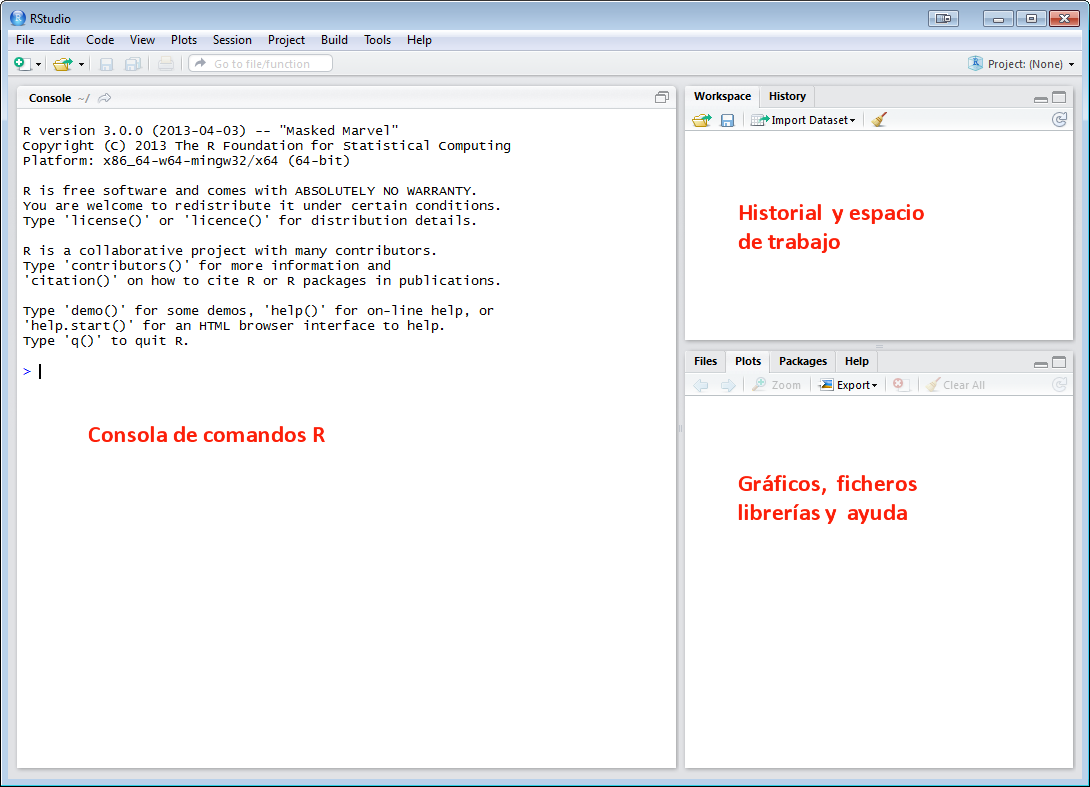
\includegraphics[height=9cm]{../fig/Tut02-01.png}
    \end{center}
Como ves, la ventana aparece dividida en tres grandes regiones o {\em paneles}, que hemos rotulado en rojo en la figura:
\begin{itemize}
  \item A la izquierda, la {\sf Consola de Comandos de R}, en la que vamos a empezar nuestro trabajo.
  \item En la parte superior derecha, el panel con las pestañas de {\sf Historial (History)},y {\sf Espacio de trabajo (Workspace)} (en versiones recientes de RStudio en lugar del {\sf Espacio de Trabajo} se muestra el {\sf Entorno (Environment)}; no te preocupes por esto de momento).
  \item En la parte inferior derecha, el panel con pestañas para {\tt Ficheros (Files)}, {\tt Gráficos (Plots)}, {\tt Librerías (Packages)} y {\tt Ayuda (Help)}. Las versiones recientes incluyen panel {\tt Visor (Viewer)}.
\end{itemize}
En este y próximos tutoriales, y con la práctica, iremos conociendo la finalidad de cada una de esas regiones. Vamos a comenzar con la {Consola de Comandos}. En ella aparecen en primer lugar una serie de mensajes con información sobre la versión de R que estamos ejecutando (la 3.0.0 en esa figura, aunque seguramente tú habrás instalado una versión superior). Y bajo estos mensajes aparece el {\tt prompt} de R, que es el símbolo {\tt >}, junto al que parpadea el cursor.\\

Ese símbolo, y el cursor parpadeando, nos indican que ese es el {\sf prompt activo}, y que R está esperando una orden. En esta primera sección, vamos a aprender a usar R (a través de RStudio) como una calculadora. El objetivo principal es que empecemos a familiarizarnos con la sintaxis de R y con las peculiaridades de la interfaz de RStudio.

Empecemos el juego. Vamos a calcular $3^2$. Asegúrate de que estás situado en la línea del prompt de R. Si es necesario, haz clic con el ratón junto al símbolo {\tt >}, y después teclea:
\begin{center}
\verb#3^2#
\end{center}
El símbolo \verb#^# es un acento circunflejo, el símbolo $\wedge$, normalmente situado junto a la {\tt P} de un teclado español estándar en Windows, y en los Mac, situado junto a la tecla {\tt fn}. Al pulsar {\tt Entrar} aparecerá una línea como esta:
\begin{center}
{\tt [1] 9}
\end{center}
%\begin{center}
%{\tt a=2}
%\end{center}
y, justo debajo,  aparece un nuevo prompt, que ahora pasa a  ser el prompt activo.
    \begin{center}
    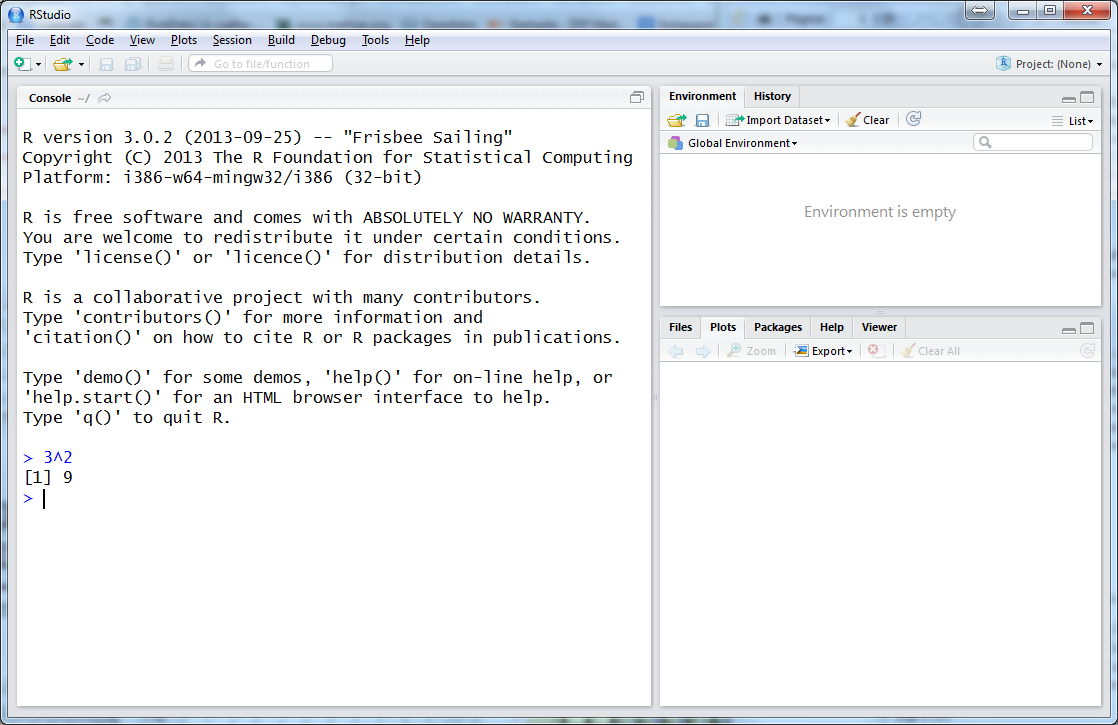
\includegraphics[height=10cm]{../fig/Tut02-02.png}
    \end{center}
%y pulsa {\tt Entrar}. En la Consola de Comandos aparece un nuevo prompt debajo, que ahora pasa a ser el prompt activo, y en el panel {\tt Workspace} aparece {\tt a} y al lado el valor 2. Lo que hemos hecho es {\sf asignar} el valor 2 a la variable {\tt a}. Vamos a elevar al cuadrado esa variable, escribiendo (en el prompt activo):
%\begin{center}
%\verb#a^2#
%\end{center}
%(Es un acento circunflejo, el símbolo $\wedge$ de tu teclado). Al pulsar {\tt Entrar} aparecerá una línea como esta:
%\begin{center}
%{\tt [1] 4}
%\end{center}
El uno entre corchetes es la forma en la que R nos indica que esta es la primera línea de su respuesta. En este caso la respuesta cabe holgadamente en una línea, pero pronto veremos casos en los que no es así.  El número $9$, naturalmente, es el valor $3^2$ que hemos calculado. Como ves, en R se usa \verb#^# para los exponentes, igual que en Calc.\\[5mm]

Las {\sf operaciones aritméticas} elementales se representan así en R (como en muchos otros programas):
\begin{itemize}
  \item suma: {\tt +}
  \item resta: {\tt -}
  \item producto: {\tt *}
  \item cociente: {\tt /}
  \item potencia: \verb#^#
  %\item cociente entero:  \verb#%/%#  (por ejemplo   $17\verb#%/%#3=5$, porque $17=3*5+2$)
  %\item resto entero:  \verb#%%#   (por ejemplo   $17\verb#%%#3=2$, porque $17=3*5+2$)
\end{itemize}

La raíz cuadrada es una {\sf función} en R, la primera que vamos a  discutir. Se representa con {\tt sqrt} (del inglés, {\em square root}). Es como en Calc, pero recuerda que, en R, la diferencia entre mayúsculas y minúsculas es, siempre, esencial; {\tt Sqrt}, o {\tt SQRT} no funcionarán. Se usa poniendo el {\sf argumento} entre paréntesis. Por ejemplo, si tecleas
{\tt sqrt(9)}
en el siguiente prompt activo, y lo ejecutas (pulsa {\tt Entrar})
obtendrás el resultado previsible:
    \begin{center}
    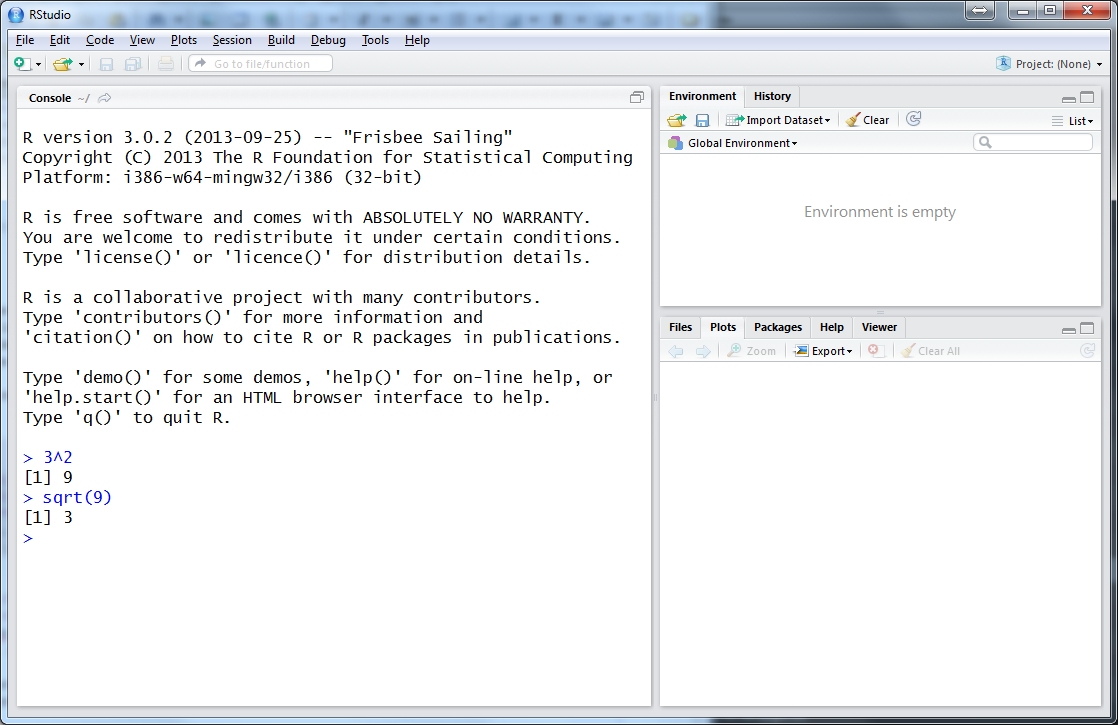
\includegraphics[height=10.5cm]{../fig/Tut02-03.png}
    \end{center}
Un aviso: aunque hasta aquí te hemos mostrado el resultado mediante figuras, con capturas de pantalla, vamos a empezar a usar cada vez más descripciones {\em textuales} como esta:
\begin{verbatim}
> sqrt(9)
[1] 3
\end{verbatim}
Sólo recurriremos a las capturas de pantalla en los casos en los que nos interesa destacar visualmente algún aspecto de la interfaz gráfica del programa. La ventaja (aparte de ahorrar espacio en el tutorial, claro) es que estas descripciones textuales te permitirán seleccionar el texto en la versión en pdf del tutorial, para usar {\em copiar y pegar} con RStudio. Ya irás viendo que esa forma de trabajar, aunque a veces tiene algún problema, a la larga te resulta cómoda. Pero, a la vez que te decimos esto, te recomendamos que, especialmente al principio, practiques tecleando tú mismo muchos de los comandos, para acostumbrarte a la interfaz, y para ayudarte a recordarlos mas eficazmente.  En las descripciones textuales, a menudo te mostraremos juntos prompt, comandos y salida; en otros casos, nos limitaremos al comando R. Recuerda, si usas {\em copiar y pegar}, que el prompt \verb#># no forma parte del comando.

Naturalmente, además de {\tt sqrt}, en R hay muchas otras funciones relacionadas con la Estadística que iremos encontrando en el resto del curso. Para practicar un poco más este uso de R como calculadora y la técnica de {\em copiar y pegar}, además de introducir un par de ideas nuevas, vamos a proponerte el primer ejercicio de este tutorial.

\begin{ejercicio}
\label{tut02:ejercicio01}
\quad\\
En este ejercicio vamos a utilizar las líneas de  código que aparecen a continuación. Copia o teclea cada línea en el prompt (¡practica las dos maneras!), una por una, y ejecútalas, pulsando {\tt Entrar} tras copiar o teclear cada línea. Trata de adivinar el resultado de cada operación antes de ejecutar el código:
\begin{verbatim}
2+3
15-7
4*6
13/5
13%/%5
13%%5
1/3+1/5
sqrt(25)
sqrt(26)
sin(pi)
sin(3.14)
\end{verbatim}
\qed
\end{ejercicio}

Los resultados de este ejercicio aparecen en la Tabla \ref{tut02:tabla:ResultadosEjercicio01} (pág. \pageref{tut02:tabla:ResultadosEjercicio01}). ¡No los mires sin haberlo intentado! Esos resultados se merecen algunos comentarios:
\begin{itemize}
  \item Seguramente, las líneas que menos previsibles te han resultado son las que contienen los operadores \verb#%/%# y \verb#%%#.
        Estos operadores representan, respectivamente, el cociente y el resto de la división entera.
  \item Lo más importante que tienes que observar en los resultados es que R trabaja {\em
        siempre} con la representación mediante decimales de los números. Esto es evidente, por ejemplo, en la respuesta a la instrucción
        \begin{verbatim}
        1/3+1/5
        \end{verbatim}
        que representa la operación
        \[\dfrac{1}{3}+\dfrac{1}{5},\]
        pero cuyo resultado en R es {\tt 0.5333333} y no {\tt 8/15}. El valor decimal es una aproximación a la fracción, pero no es un resultado exacto (la fracción sí es exacta). Por lo tanto, cuando hagamos operaciones con R, tenemos que tener cuidado con la posible pérdida de precisión, que llevan siempre aparejadas las operaciones con decimales. Técnicamente, esto significa que R es un programa (esencialmente) {\sf numérico}. Más adelante en el curso veremos algún programa {\sf simbólico}, y discutiremos la diferencia entre ambos.
        \begin{table}[t!]
\hrule
\quad
\begin{verbatim}
                    > 3^2
                    [1] 9
                    > sqrt(9)
                    [1] 3
                    > 2+3
                    [1] 5
                    > 15-7
                    [1] 8
                    > 4*6
                    [1] 24
                    > 13/5
                    [1] 2.6
                    > 13%/%5
                    [1] 2
                    > 13%%5
                    [1] 3
                    > 1/3+1/5
                    [1] 0.5333333
                    > sqrt(25)
                    [1] 5
                    > sqrt(26)
                    [1] 5.09902
                    > sin(pi)
                    [1] 1.224606e-16
                    > sin(3.14)
                    [1] 0.001592653
\end{verbatim}
\caption{Resultados del Ejercicio \ref{tut02:ejercicio01}.}
\label{tut02:tabla:ResultadosEjercicio01}
\hrule
\end{table}

  \item Fíjate en que, como hemos dicho, R ha interpretado el símbolo
        \begin{verbatim}
        1/3+1/5
        \end{verbatim}
        como la operación
        \[\dfrac{1}{3}+\dfrac{1}{5},\]
        en lugar de darle otras interpretaciones posibles como, por ejemplo:
        \[\dfrac{1}{\left(\dfrac{3+1}{5}\right)}.\]
        Para hacer esa interpretación R ha aplicado una serie de reglas, de lo que se conoce como {\sf prioridad de operadores}, y que dicen en que orden se realizan las operaciones, según el tipo de operador. No queremos entretenernos con esto ahora, así que baste con decir que, en caso de duda, siempre puedes (y a menudo, debes) usar paréntesis para despejar la posible ambigüedad.
        \newpage

        Por ejemplo, para distinguir entre las dos interpretaciones que hemos dado, puedes escribir:
        \begin{verbatim}
        (1/3)+(1/5)
        \end{verbatim}
        o, por el contrario,
        \begin{verbatim}
        1 /( (3+1)/5 )
        \end{verbatim}
        Un uso prudente de paréntesis y espacios en las operaciones es una marca característica del buen hacer, cuando se escribe código en un ordenador. Si alguna vez esto llega a ser un problema para ti, habrá llegado el momento de aprender algo más sobre esa {\em prioridad de operadores}.

  \item La función {\tt sin} es la función {\em seno} de la Trigonometría. Además, R utiliza el símbolo {\tt pi} para referirse a la constante matemática $\pi\approx 3.141593$. Y el carácter numérico de R se refleja, de nuevo, en el hecho de que al ejecutar {\tt sin(pi)} no has obtenido $0$ (que es la respuesta exacta), sino:
      \begin{verbatim}
      > sin(pi)
      [1] 1.224606e-16
      \end{verbatim}
      La notación que se usa en la respuesta es la forma típica de traducir la {\sf notación científica} a los lenguajes de ordenador y calculadoras. El símbolo {\tt 1.224606e-16} representa el número:
      \[1.224606\cdot 10^{-16},\]
      de manera que el número {\tt -16}, que sigue a la letra {\tt e} en esta representación, es el {\sf exponente} de $10$ (también llamado {\sf orden de magnitud}), mientras que el número {\tt 1.224606} se denomina a veces {\sf mantisa}. Puedes leer más sobre la notación científica en este artículo de la Wikipedia:
      \begin{center}
      \link{http://es.wikipedia.org/wiki/Notaci\%C3\%B3n\_cient\%C3\%ADfica}{http://es.wikipedia.org/wiki/Notación\_científica}
      \end{center}
      En cualquier caso, el exponente {\tt -16} nos indica que se trata de un número extremadamente cercano a $0$. Fíjate, en cambio, que si usas $3.14$ como aproximación de $\pi$, la respuesta, aunque pequeña, es todavía del orden de milésimas.
\end{itemize}

\subsection{Algunos detalles de la interfaz de RStudio.}
\label{tut02:subsec:AlgunosDetallesInterfazRStudio}

Antes de avanzar más, queremos ocuparnos de algunos aspectos del trabajo con RStudio que a menudo causan algunos quebraderos de cabeza a quienes se inician en el uso del programa.

\subsubsection*{Comandos incompletos}

Para ver un ejemplo, prueba a escribir, en el prompt activo, esta operación evidentemente incompleta:
\begin{verbatim}
3*
\end{verbatim}
y pulsa {\tt Entrar}. La respuesta de R es un símbolo {\tt +}:
\begin{verbatim}
> 3*
+
\end{verbatim}
que en este caso no tiene nada que ver con la suma. Es la forma que tiene R de decirnos ``necesito algo {\em más}''. Cuando R se encuentra con una expresión que considera no errónea, sino incompleta (por ejemplo, con un paréntesis abierto al que corresponde un paréntesis cerrado), entonces nos lo comunica con este símbolo {\tt +}. Y al hacerlo, nos da la oportunidad, en casos como este, de corregir el error, completando la expresión incompleta. Así que si, ahora, junto al símbolo {\tt +} escribes $2$, de esta forma:
\begin{verbatim}
> 3*
+ 2
\end{verbatim}
y pulsas {\tt Entrar}, verás que R ha entendido la expresión completa {\tt 3*2} y nso devuelve la respuesta:
\begin{verbatim}
> 3*
+ 2
[1] 6
\end{verbatim}
En algún momento, no obstante, ese símbolo {\tt +} de los comandos incompletos se convertirá en un inconveniente. Imagínate, por ejemplo, que querías multiplicar $5\cdot 7$, pero que por error has tecleado la expresión
\begin{verbatim}
5*7-
\end{verbatim}
y has pulsado {\tt Entrar}, antes de darte cuenta del error. En tal caso, R piensa que esa expresión está incompleta, y vuelve a aparecer el signo {\tt +}
\begin{verbatim}
> 5*7-
+
\end{verbatim}
¡Pero ahora no queremos añadir nada! En este caso podrías añadir un $0$, sin que eso afectara el resultado.  pero habrá, más adelante, muchos casos en los que no hay una solución sencilla evidente. ¿Cómo salimos del paso? Simplemente, pulsamos la tecla {\tt Esc} (escape), con lo que R interrumpe el comando y nos devuelve a un nuevo prompt activo, sin calcular nada.

\subsubsection*{Navegando el historial de comandos}

En un caso como el que hemos descrito, no supone un problema volver a teclear la expresión, evitando el error que habíamos cometido. Pero en ocasiones, si hemos escrito una expresión realmente complicada, y, por ejemplo, hemos tecleado un paréntesis de más en medio de la expresión, seguramente preferiríamos no tener que volver a teclear la expresión completa. Un remedio ``casero'' consiste en seleccionar y copiar la expresión errónea, pegarla en el prompt activo, y editarla ahí para corregir el error.

Hay una segunda manera de conseguir el mismo efecto, Otra característica interesante de la Consola de Comandos es que, si te sitúas en el prompt activo, y pulsas las teclas con flechas arriba o abajo, verás pasar la lista completa de comandos que has ejecutado,  desde el principio de la sesión de trabajo. Prueba a hacerlo ahora, para ver como funciona. Si has ejecutado todos los comandos que hemos ido describiendo en este tutorial, puedes pulsar la flecha $\uparrow$ repetidamente, e irás viendo pasar todos esos comandos, hasta llegar al
\begin{verbatim}
3^2
\end{verbatim}
con el que hemos empezado. Y con la flecha hacia abajo recorres la lista en sentido contrario, hasta el comando de ejecución más reciente. Esa lista de comandos es el {\sf Historial de Comandos}. Usando las flechas arriba y abajo puedes recorrer el Historial de Comandos, detenerte en cualquier punto, modificar ese comando si lo deseas, y después ejecutarlo (con o sin modificaciones). Al principio puede que te cueste un poco acostumbrarte, pero una vez que te habitúes a esta herramienta, la encontrarás, sin duda, muy útil.
El Historial de Comandos que puedes recorrer con las flechas arriba y abajo se limita a la sesión de trabajo actual. Pero si miras en el panel superior derecho de RStudio, verás una pestaña titulada {\tt History}, que se muestra en esta figura:
    \begin{center}
    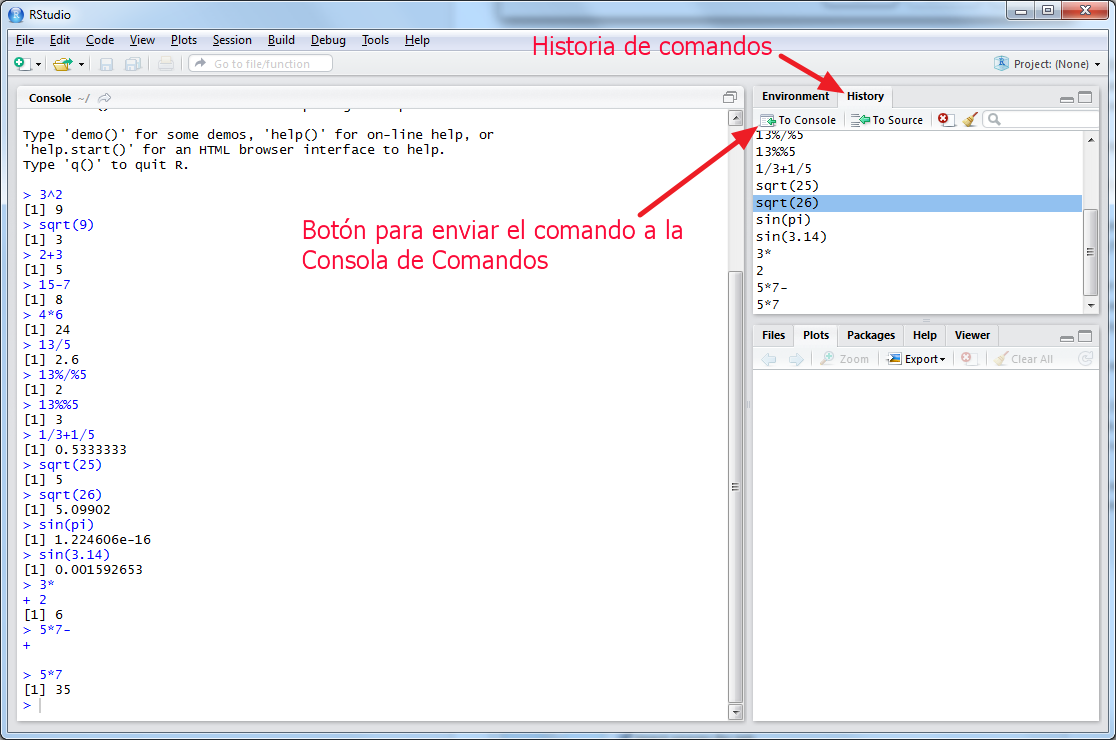
\includegraphics[height=10cm]{../fig/Tut02-04.png}
    \end{center}
El Historial de Comandos que aparece en ese panel refleja tus comandos de esta y anteriores sesiones. Si esta es tu primera sesión de trabajo con R, ambos coincidirán, claro está. Pero a medida que vayas abriendo RStudio en días sucesivos, te puede resultar muy útil localizar, por ejemplo, un comando que usaste hace dos sesiones, pero que no recuerdas exactamente. Los comandos que aparecen en ese panel se pueden copiar y pegar en la Consola de Comandos o, de forma más directa, puedes seleccionar uno de ellos con el ratón, y pulsar en el botón {\tt To Console} que hemos destacado en la Figura.

\subsubsection{Errores.}

Los errores son inevitables, y nos conviene estar preparados para su aparición. Dependiendo del motivo del error, R nos informará con distintos tipos de mensajes. Así que vamos a ver algunos ejemplos, para conocer la terminología asociada.

Para empezar, este es el mensaje de error que obtenemos tras ejecutar una expresión sin sentido:\\

\begin{tabular}{l}
{\tt > 4/*3}\\
\textcolor{red}{\tt Error: unexpected '*' in "4/*"{}}
\end{tabular}\\

Los mensajes de error aparecen en color rojo en RStudio. Este mensaje de error en particular, es bastante fácil de entender: R simplemente se queja de que esta expresión es defectuosa. No incompleta, como alguna que hemos visto antes. Es imposible completar esta expresión de forma correcta.

Veamos otro tipo de mensaje de error. Ya sabes  que no se puede dividir por $0$. Si lo intentamos en R
\begin{verbatim}
> 2/0
[1] Inf
\end{verbatim}
el símbolo {\tt Inf} (de infinito) nos avisa del problema. Ese símbolo también puede aparecer con signo menos, si por ejemplo tratas de calcular el logaritmo neperiano de $0$. En R el logaritmo neperiano es la función {\tt log}, así que sería:
\begin{verbatim}
> log(0)
[1] -Inf
\end{verbatim}
En ambos casos R no lanza un mensaje de error, pero utiliza el símbolo de infinito, porque así nos proporciona más información matemática sobre lo que ha ocurrido. También puede suceder que el símbolo {\tt Inf} aparezca como {\em resultado intermedio} en una expresión. En ese caso R aplica unas reglas sencillas de {\em aritmética con infinitos}, para tratar de darnos la respuesta más coherente desde el punto de vista matemático. Por ejemplo, si calculas
\begin{verbatim}
3*(-5/(4-2^2))
\end{verbatim}
Entonces R empieza calculando el resultado del paréntesis {\tt 4-2\^{}2}, que es $0$. Así que al dividir $-5$ entre $0$, R obtiene {\tt -Inf}, y finalmente, al calcular {\tt 3*(-Inf)}, se obtiene {\tt -Inf} como valor de la expresión. Comprobémoslo:
\begin{verbatim}
> 3*(-5/(4-2^2))
[1] -Inf
\end{verbatim}
A pesar de que R no lanza mensajes de error, está claro que, en la mayoría de los casos,  no es deseable que nuestros cálculos produzcan {\tt Inf} como resultado, en ninguna etapa.

En otros casos, el problema es diferente. Por ejemplo, si tratas de calcular la raíz cuadrada de un número negativo:\\

\begin{tabular}{l}
{\tt > sqrt(-4)}\\
{\tt [1] NaN}\\
\textcolor{red}{\tt Warning message:{}}\\
\textcolor{red}{\tt In sqrt(-4) : NaNs produced{}}
\end{tabular}\\
En este caso obtenemos una respuesta {\tt NaN}, y además una advertencia ({\em warning}) sobre la aparición de esa respuesta. El símbolo {\tt NaN} es la abreviatura de {\em Not a Number}; es decir ``no es un número''. Esta es la respuesta que obtendremos cuando tratamos de hacer operaciones como esta, que producen como resultado un número complejo. R es capaz de trabajar con los números complejos, pero como no los vamos a necesitar en el curso, no nos ocuparemos de esto. Para que veas otro ejemplo, esa respuesta {\tt NaN} aparece también si tratamos de ir demasiado lejos con la {\em aritmética con infinitos:}
\begin{verbatim}
> (1/0)+log(0)
[1] NaN
\end{verbatim}
En este caso R se ha encontrado en un paso intermedio con {\tt Inf - Inf}, y su respuesta ha sido {\tt NaN}.\\

En cualquier caso, y como resumen final,  tenemos que tratar de evitar que nuestros cálculos conduzcan a este tipo de expresiones.




\subsubsection*{Haciendo limpieza en la Consola de Comandos.}

Si has seguido todas las instrucciones hasta aquí, tu Consola de Comandos seguramente empieza a estar llena de comandos, y algunos pueden quedar ocultos en la parte superior. Naturalmente, puedes usar las barras de desplazamiento para moverte por la Consola. Pero en sesiones largas de trabajo, o cuando hemos terminado de hacer pruebas y queremos ejecutar una versión definitiva de nuestro trabajo, es normal que queramos hacer limpieza en la Consola. Eso se consigue con la combinación de teclas {\tt Ctrl + L}. ¡Cuidado! Es un proceso no reversible: podrás seguir navegando el Historial de  Comandos con las teclas arriba y abajo, pero para recuperar los resultados tendrás que ejecutar de nuevo los comandos.

Más adelante aprenderemos formas de guardar nuestro trabajo de una manera más eficiente. Pero te podemos adelantar que, puesto R se maneja {\em escribiendo comandos}, bastará con guardar esos comandos en ficheros de texto plano. Ahora vamos a cambiar de tema, y para empezar desde cero, vamos a cerrar RStudio para eliminar las trazas del trabajo que hemos hecho.

%Cerraremos RStudio y volveremos a abrirlo. Más adelante en el curso aprenderemos formas más sofisticadas de hacer limpieza, pero por hoy esto será suficiente. Cuando cierres RStudio, aparecerá una pregunta como esta:
%    \begin{center}
%    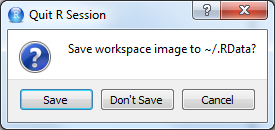
\includegraphics[height=3cm]{../fig/Tut03-15.png}
%    \end{center}
%Puedes pulsar sobre {\tt Don't Save} sin preocupaciones, ya aprenderás más adelante el significado de la pregunta.


\section{Variables y vectores.}

Vuelve a abrir RStudio, para continuar el trabajo. En la sección previa hemos usado R como una calculadora. Pero, para ir más allá, tenemos que disponer de {\em estructuras de datos}. Ese término describe, en Computación, las herramientas que nos permiten almacenar y procesar información. Las estructuras de datos más básicas de R son las {\sf variables} y los {\sf vectores}. En próximos tutoriales nos iremos encontrando con otras estructuras de datos: {\sf matrices}, {\sf data.frames}, {\sf listas}, entre otras.

\subsection{Variables en R.}

Una {\sf variable}, en R, es un símbolo que usamos para referirnos a un valor. Por ejemplo, si te sitúas en la Consola de Comandos, tecleas
\begin{verbatim}
a = 2
\end{verbatim}
y ejecutas esa instrucción, entonces, aunque aparentemente no ha sucedido nada (porque no hay respuesta), a partir de ese momento R ha asignado el valor 2 al símbolo {\tt a}. Así que si, por ejemplo, tecleas y ejecutas
\begin{verbatim}
a + 1
\end{verbatim}
obtendrás como respuesta $3$.
\begin{ejercicio}
\label{tut02:ejercicio02}
\quad\\
¿Qué se obtiene al ejecutar estos comandos, uno detrás de otro? ¿Cuánto valen las variables {\tt a}, {\tt b} y {\tt c} al final?
\begin{verbatim}
a = 2
b = 3
c = a + b
a = b * c
b = (c - a)^2
c = a * b
\end{verbatim}
La solución está en la página \pageref{tut02:ejercicio02:sol}. ¡No la mires antes de intentar pensar el ejercicio por ti mismo!
\qed
\end{ejercicio}

En el Capítulo \ref{curso-cap:IntroduccionEstadisticaDescriptiva} del libro hemos hablado de variables cualitativas y cuantitativas. Estas últimas toman siempre valores numéricos, y las variables de R sirven, desde luego, para almacenar esa clase de valores. Pero, como iremos viendo en sucesivos tutoriales,  también se pueden utilizar variables de R para guardar valores de variables cualitativas (factores), y  otros tipos de objetos que iremos conociendo a lo largo del curso. De momento, para que veas a que nos referimos, recordaremos el Ejemplo \ref{curso-cap01:ejem:VariableCualitativaOrdenada} del libro (pág. \pageref{curso-cap01:ejem:VariableCualitativaOrdenada}), en el que teníamos una variable cualitativa ordenada que representa el pronóstico de un paciente que ingresa en un hospital. Prueba a ejecutar este código:

\begin{verbatim}
pronostico = "Leve"
\end{verbatim}
simplemente para que, de momento, veas que:
\begin{itemize}
  \item R no protesta. El valor \verb#"Leve"# es un valor perfectamente aceptable.
  \item En R los valores que representan palabras, frases, o como las llamaremos técnicamente {\sf cadenas alfanuméricas}, se escriben siempre entre comillas. Puedes usar comillas simples o dobles, pero te aconsejamos que uses dobles comillas.
\end{itemize}
La relación entre factores y valores alfanuméricos en R es algo más complicada de lo que este sencillo ejemplo parece sugerir. Pero ya tendremos ocasión, en futuros tutoriales, de extendernos sobre eso.


\subsubsection*{Asignaciones}

Las instrucciones como
\begin{verbatim}
a = 2
\end{verbatim}
o como
\begin{verbatim}
b = (c - a)^2
\end{verbatim}
se denominan {\tt asignaciones}. En la primera, por ejemplo, decimos que hemos asignado el valor {\tt 2} a la variable {\tt a}.

Queremos advertir al lector de que en R hay otra forma, esencialmente equivalente, de escribir las instrucciones, y que, de hecho, se usa mayoritariamente. En lugar del símbolo {\tt =}, puedes conseguir el mismo efecto escribiendo {\tt <-} (el signo ``menor'' seguido, sin espacios, de un signo ``menos''). Así que, si ejecutas
\begin{verbatim}
a <- 2
\end{verbatim}
el resultado será el mismo que antes con {\tt =}. Las dos notaciones tienen ventajas e inconvenientes, pero nosotros preferimos {\tt =} porque se parece más a lo que se utiliza en muchos lenguajes de programación.
\subsubsection*{Cómo ver los resultados de un cálculo a la vez que lo hacemos}

Ya habrás notado que, al hacer una asignación, R no produce ninguna respuesta, y se limita a guardar el valor en la variable. En una asignación como {\tt a=2}, esto no genera ninguna duda. Pero si el miembro derecho de la asignación es una expresión más complicada, puede ser conveniente pedirle a R que nos muestre  el resultado de esa expresión {\em a la vez } que se hace la asignación. Imagínate, por ejemplo, esta situación:
\begin{verbatim}
b =  2
c = -2
d = -4
a = b * c^2 / d + 3
\end{verbatim}
¿Cuál es el valor que se asigna a la variable {\tt a}? Una forma de averiguarlo es, simplemente, ejecutar una línea adicional, en la que aparece sólo el nombre de la variable que queremos inspeccionar. Al ejecutar esta sentencia, R nos devuelve como respuesta:
\begin{verbatim}
> a
[1] 1
\end{verbatim}
Pero hay otra manera de conseguir que R nos muestre el resultado de la asignación que es más interesante, porque produce código más simple. Basta con encerrar toda la asignación entre paréntesis. El resultado es:
\begin{verbatim}
> ( a = b * c^2 / d + 3 )
[1] 1
\end{verbatim}
como antes. Este ejemplo es, desde luego, bastante artificial.  Te recordamos, en cualquier caso, la conveniencia de utilizar paréntesis para hacer más legibles las expresiones, y evitar posibles errores. Pero, a la vez, la posibilidad de comprobar el resultado de las asignaciones, aumenta la fiabilidad del código que escribimos.

\subsubsection*{Nombres de las variables}

Aunque hasta ahora hemos usado letras como nombres de las variables, puedes utilizar nombres más descriptivos. Y muchas veces es una buena idea hacerlo. Por ejemplo,  puede que hace una semana hayas escrito estas instrucciones para resolver un problema:
\begin{verbatim}
a = 2
b = 3
c = a / b
\end{verbatim}
Pero si las vuelves a ver, pasada una semana, es posible que no recuerdes qué era lo que estabas tratando de conseguir al hacer esto. En cambio, al ver estas instrucciones:
\begin{verbatim}
espacio = 2
tiempo = 3
velocidad = espacio / tiempo
\end{verbatim}
es mucho más fácil reconocer el objetivo que persiguen. A lo largo de los tutoriales del curso vamos a insistir muchas veces en la necesidad de que el código esté bien {\em organizado}, y esté bien {\em documentado}. Un primer paso en esa dirección es tratar de elegir nombres descriptivos para las variables. En R las reglas para los nombres de variables son muy flexibles: esencialmente, que empiecen por una letra y no contengan espacios ni caracteres especiales, como {\tt ?}, {\tt +}, paréntesis, etcétera. Pero cuidado con los excesos. Es cierto que puedes usar nombres de variables arbitrariamente largos.  Pero si usas como nombre:
\begin{verbatim}
Estavariablealmacenaelresultadodelaoperaciontaninteresantequeacabamosdehacer
\end{verbatim}
tu trabajo resultará ilegible. Como siempre, se necesita un equilibrio, y con la práctica encontrarás el tuyo (consejo zen gratuito del tutorial de hoy). Para empezar, es una buena idea combinar mayúsculas y minúsculas en los nombres de las variables. Si  vas a usar una variable para representar la temperatura final de un proceso, el nombre {\tt temperaturafinalproceso} es menos legible y más largo que {\tt tempFinal}. Es mucho más fácil, por otra parte, que te equivoques tecleando el primero de esos nombres.

\subsection{Vectores.}

En Estadística, lo habitual es trabajar con colecciones o {\em muestras} de datos. Y para almacenar esas colecciones de datos, la estructura más básica de R son los vectores. En este apartado vamos a empezar nuestro trabajo con ellos, aunque a lo largo del curso aún tendremos ocasión de aprender bastante más sobre el manejo de los vectores de R.

Para empezar vamos a trabajar con vectores que contienen una colección de números, que pueden ser las edades de los alumnos de una clase:
\begin{center}
22, 21, 18, 19, 17, 21, 18, 20, 17, 18, 17, 22, 20, 19, 18, 19, 18, 22, 20, 19
\end{center}
En R, las listas de números como esta se almacenan en vectores. El vector que corresponde a esas edades se construye en R mediante un comando como este:
{\small
\begin{verbatim}
edades = c(22, 21, 18, 19, 17, 21, 18, 20, 17, 18, 17, 22, 20, 19, 18, 19, 18, 22, 20, 19)
\end{verbatim}
}
En realidad, en esa expresión hemos hecho dos cosas:
\begin{enumerate}
  \item Hemos {\em creado} el vector con los datos, en la parte derecha de la expresión:
    {\small
    \begin{verbatim}
    c(22, 21, 18, 19, 17, 21, 18, 20, 17, 18, 17, 22, 20, 19, 18, 19, 18, 22, 20, 19)
    \end{verbatim}
    }
    Los datos están separados por comas, y rodeados por paréntesis. Hasta aquí todo es bastante típico, pero {\em fíjate especialmente en la letra} {\tt c} que precede al primer paréntesis. Esa letra {\tt c} es el nombre de una nueva función de R, y es la forma más sencilla que existe en R para crear un vector de datos. Podría pensarse que la c es de {\em crear}, pero en realidad proviene de {\em concatenar}. Enseguida entenderemos porque es así.

  \item Una vez creado el vector, lo hemos {\em asignado} a la variable {\tt edades}. Hasta ahora sólo habíamos usado variables para identificar un único valor (un número o una cadena alfanumérica). Pero una variable puede usarse para identificar un vector o, como  veremos más adelante, estructuras mucho más complejas.

\end{enumerate}
Una observación más: los vectores de R se usan para almacenar valores de una variable. Y en particular, todos los datos de un vector son del mismo tipo de variable. No se puede mezclar, en un vector, números y cadenas alfanuméricas (aparentemente R te dejará hacerlo, pero internamente habrá convertido todos los números en cadenas alfanuméricas).\\

Manos a la obra. Prueba a copiar el comando anterior en tu {\em Consola de comandos} (puedes usar {\em copiar y pegar} desde este fichero) y ejecútalo. Si las cosas van bien, no esperes ninguna respuesta: como ya hemos dicho, R no te muestra el resultado de las asignaciones. Recuerda que, si quieres ver el resultado de una asignación, puedes rodear toda línea con paréntesis, como en:
{\small
\begin{verbatim}
(edades = c(22, 21, 18, 19, 17, 21, 18, 20, 17, 18, 17, 22, 20, 19, 18, 19, 18, 22, 20, 19))
\end{verbatim}
}
Otra opción, naturalmente, es preguntarle a R por el valor de {\tt edades}, después de la asignación. Escribe simplemente {\tt edades} en la {\em Consola de Comandos} y ejecútalo. Verás, de nuevo, el contenido de esa variable.\\

Vamos a hacer algunas operaciones con este vector. Imagínate que, como sucede a menudo, después de haber creado nuestra lista de edades de alumnos, desde la administración nos avisan de que hay cinco alumnos nuevos, recién matriculados, y debemos incorporar sus edades, que son
\begin{center}
22, 18, 20, 21, 20
\end{center}
a nuestro vector de datos. Naturalmente, podemos empezar de nuevo, pero es preferible reutilizar el vector {\tt edades} que ya habíamos creado. Vamos a ver esto como primer ejemplo, para empezar a aprender cómo se manipulan vectores en R. Una forma de añadir los datos es empezar creando un nuevo vector (con la función {\tt c} de R):
\begin{center}
{\tt
(edades2 = c(22, 18, 20, 21, 20))
}
\end{center}
Y a continuación {\em concatenamos} los vectores, usando de nuevo la misma función {\tt c}, de una manera distinta:
\begin{center}
{\tt
(edades = c( edades, edades2))
}
\end{center}
Hemos rodeado toda la línea con paréntesis, para ver el resultado y poder observar cómo ha cambiado el vector {\tt edades}.


Vamos a analizar paso a paso lo que ha ocurrido:
\begin{itemize}
  \item La instrucción {\tt c( edades, edades2)} toma los datos contenidos en {\tt edades} y {\tt edades2} y los {\em concatena}, en ese orden, para fabricar un nuevo vector, que todavía no está guardado en ninguna variable.

  \item La asignación {\tt edades = c( edades, edades2)} toma ese vector y lo guarda en la propia variable {\tt edades}. Al hacer esto, como era de esperar, el anterior vector {\tt edades} es reemplazado con la nueva lista, y su contenido anterior se pierde (cuidado con esto; las reasignaciones son una de las formas habituales de cometer errores).
\end{itemize}
El nombre de la función {\tt c} proviene, en realidad, de {\em concatenate}, concatenar en inglés.



La siguiente figura resume lo que hemos venido haciendo con estos datos:
    \begin{center}
    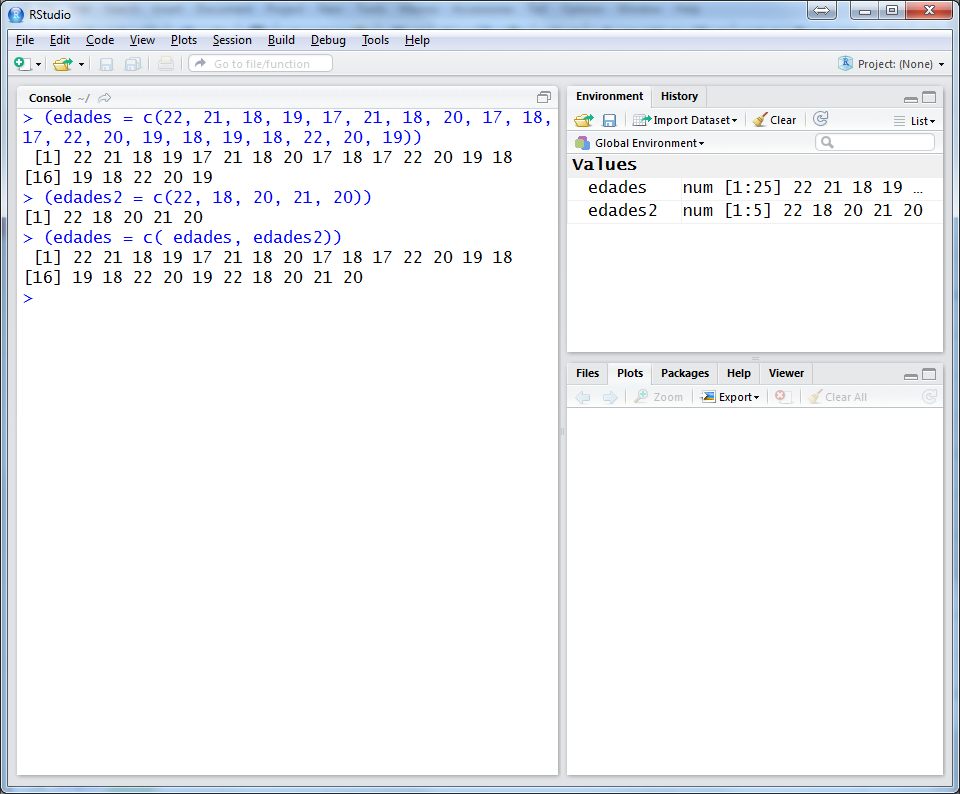
\includegraphics[height=7cm]{../fig/Tut02-05.png}
    \end{center}
Los números entre corchetes, al principio de cada fila, como el {\tt [1]} y el {\tt [16]} de este ejemplo, son sólo ayudas para que podamos localizar los elementos del vector. En mi pantalla la primera fila muestra los primeros $15$ números del vector. Pero en la tuya, si la ventana de RStudio es de distinta anchura, los números entre corchetes pueden ser distintos. Hasta ahora sólo habíamos visto ejemplos con {\tt [1]}, que es lo que sucede cuando la respuesta es un vector que cabe en una única línea.



\section{Ficheros {\tt csv} con R.}
\label{tut03:sec:FicherosCsvEnR}

En esta sección vamos a aprender a utilizar ficheros {\tt csv} con R. En el Tutorial-01 hemos visto algunos ejemplos de ese tipo de ficheros, y el manejo básico con una hoja de cálculo, como Calc. Como vimos allí, un fichero {\tt csv} típico contiene una tabla de datos, con varias columnas. Esa estructura de tabla se hará imprescindible más adelante. Pero durante una buena parte del curso, nosotros nos vamos a limitar a problemas en los que interviene una única variable. En tal caso, para almacenar los datos de esa variable nos podemos a limitar a considerar un tipo de ficheros {\tt csv} muy básico, como el fichero adjunto:
\begin{center}
\fichero{../datos/Tut02-Edades.csv}{Tut02-Edades.csv}
\end{center}
Guárdalo en la subcarpeta {\tt datos} de tu directorio de trabajo (el que contiene este pdf). Si lo abres con un editor de texto (como el {\em Bloc de Notas}, en Windows), verás, como muestra esta figura,

    \begin{center}
    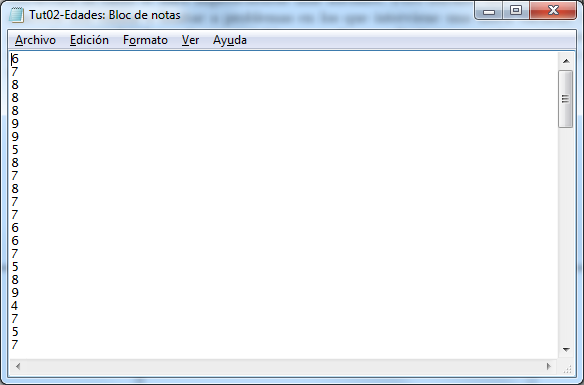
\includegraphics[height=8cm]{../fig/Tut02-06.png}
    \end{center}

que el fichero contiene  sólo una columna de datos, que en este ejemplo corresponde a valores de una variable cuantitativa discreta. En la figura sólo se muestra una parte de los datos.
%Asegúrate de que has guardado este fichero en el {\em Escritorio} de tu máquina.

\begin{ejercicio}
\label{tut02:ejercicio03}
\quad\\
¿Cuántos datos hay en ese vector? Usa Calc para averiguarlo, pronto aprenderemos a hacerlo con R.
Solución en la página \pageref{tut02:ejercicio03:sol}.
\qed
\end{ejercicio}

%Fíjate que, como decíamos, es un tipo especial de fichero {\tt csv}, porque sólo hay una columna de datos. Más adelante en el curso necesitaremos ficheros {\tt csv} como los primeros ejemplos que hemos visto, en los que había varias columnas, con los valores de distintas variables, cada uno ocupando una columna. Piensa, para fijar ideas, en el ejemplo del fichero  {\tt Tut01-PracticaConCalc.csv} del primer tutorial, en el que teníamos tres columnas que corresponden a tres variables, como se ve en esta otra figura:
%        \begin{center}
%        \includegraphics[height=9cm]{../fig/Tut01-Calc-csv-04.png}
%        \end{center}
Queremos utilizar esos datos en R, y para eso vamos a (1) leerlos desde el fichero y (2)guardarlos en un vector. El resultado será como si nosotros hubiéramos creado ese vector tecleándo sus elementos directamente.

Para el primer paso (la lectura del fichero {\tt csv}), vamos a tener que empezar por explicarle a R (usando RStudio como intermediario), donde está el fichero que contiene esos datos. Cuando trabajamos con ficheros, R utiliza un directorio de nuestro ordenador como {\sf directorio de trabajo}. A continuación vamos a aprender a elegir un directorio de trabajo. Puedes usar cualquier carpeta, y en lo que sigue vamos a suponer que hemos elegido el {\em Escritorio}. Lo más importante es que esa carpeta debe contener a su vez, una subcarpeta llamada {\tt datos}. Y asegúrate de que los ficheros {\tt csv} que vas a usar están almacenados en esa subcarpeta llamada {\tt datos}.\\

Usamos el menú {\tt Session $\to$ Set Working Directory $\to$ Choose Directory}.
    \begin{center}
    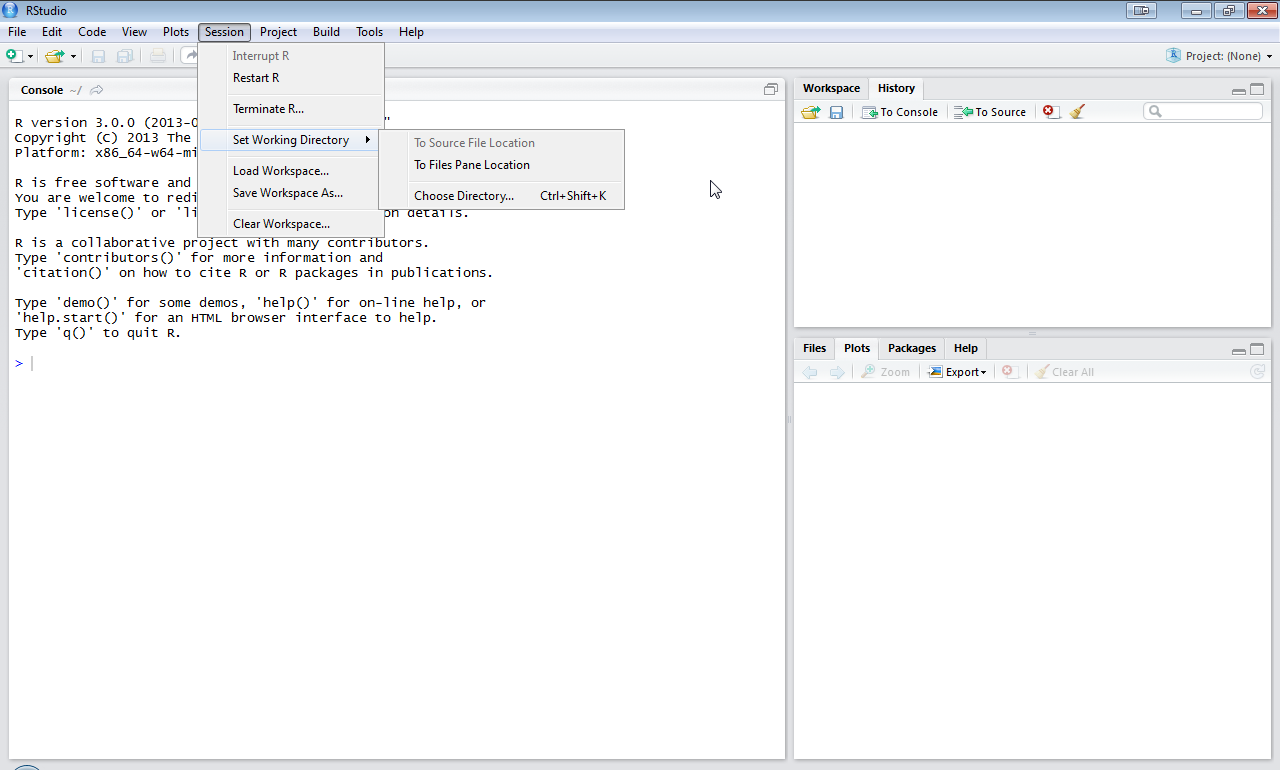
\includegraphics[height=8.5cm]{../fig/Tut03-18.png}
    \end{center}
Se abre un cuadro de diálogo del sistema, y navegamos hasta la carpeta que contiene el fichero {\tt csv}, que en mi caso es el {\tt Escritorio}. Cuando selecciono el Escritorio, veo aparecer en la Consola de Comandos de R, un comando, que RStudio ha escrito y ejecutado por nosotros:

\begin{center}
\verb# setwd("C:/Users/Fernando/Desktop") #
\end{center}
\paragraph*{}\label{tut02:lugar:ComandoSetwd}Este es el resultado en mi ordenador (de ahí el nombre de usuario), usando Windows 10. En versiones más antiguas de Windows, o en una máquina con Linux, o un Mac, el comando será ligeramente distinto. Cuando tengamos más práctica, aprenderemos otras formas de seleccionar el directorio de trabajo, o incluso de utilizar ficheros situados fuera de ese directorio de trabajo. Pero, por el momento, resulta más cómodo dejar que \mbox{RStudio} haga ese trabajo para nosotros.

% Naturalmente, ese comando incluye mi nombre de usuario. El truco para que no dependa es usar:
%
%    (dirTrabajo=paste("C:/Users/",Sys.info()["user"],"/Desktop",sep=""))
%    setwd(dirTrabajo)
%    # En sistemas Mac o Linux alguna de estas lineas (descomentar) debería tener el mismo efecto.
%    # setwd("~/Desktop")
%    # setwd("~/Escritorio")

Ahora R ya sabe dónde está el fichero que nos interesa, pero todavía no sabe cual es. Para ello vamos a utilizar la función {\tt read.table} de R. Aunque esta función tiene muchas opciones disponibles, nuestro primer uso de ella será bastante sencillo. Copia y ejecuta el siguiente código en RStudio:
\begin{center}
\begin{minipage}{10cm}
{\tt
(vectorEdades = read.table("./datos/Tut02-Edades.csv", header = FALSE)[,1])
}
\end{minipage}
\end{center}
En esta instrucción le decimos a R que use la función {\tt read.table} para leer el contenido del fichero {\tt Tut02-Edades.csv}, y que almacene lo que ha leído en un vector, que hemos decidido llamar {\tt vectorEdades}. Y aunque no es necesario entender en detalle el funcionamiento de {\tt read.table} en este momento, vamos a explicar un poco más lo que hemos hecho. A medida que el curso avance irás teniendo más ocasiones de practicar esto e irá quedando cada vez más claro. 

La opción {\tt header = FALSE} sirver para indicarle a R que la tabla almacenada en el fichero no tiene una línea de cabecera (en inglés, {\em header}) que, cuando existe, suele contener los nombres de las variables de la tabla. Además, la función {\tt read.table} sirve para leer tablas con varias columnas, obteniendo como resultado un objeto de R de tipo {\tt data.frame}. Pero nuestro primer ejemplo es muy sencillo y la tabla sólo tiene una columna. Así que usamos la notación {\tt [,1]} para indicarle a R que sólo queremos la primera columna de esa tabla, considerada como un vector.

Al ejecutar esa orden habrás obtenido una respuesta como esta: 
% (que, de paso, te puede servir para obtener la solución del Ejercicio \ref{tut02:ejercicio03}, pág. \pageref{tut02:ejercicio03}, usando la función {\tt length})
\begin{center}
\begin{tabular}{l}
{\tt > > (vectorEdades = read.table("./datos/Tut02-Edades.csv", header = FALSE)[,1])}\\
{\tt     [1]  6  7  8  8  8  9  9  5  8  7  8  7  7  6  6  7  5  8  9  4  7  5  7}\\
{\tt  [24]  7  5  9  4  7  7  7  8  5  8  9  7  4  6  6  6  9  8  6  7  6  7  6}\\
{\tt   [47]  6  8  6  5  5  6  6  8  5  8  5  9  7  6  9  5  7  8  8  7 10  7  8}\\
{\tt  [70]  7  5  6  8  8  7  3  5  6  7  5  7  7  5  8  4  8  8  8  6  7  6  6}\\
{\tt  [93]  8  5  6  5  8  6  9  7}
\end{tabular}
\end{center}
Como hemos dicho antes, los números entre corchetes, al principio de cada fila, que en mi caso son {\tt [1], [24]  [47], [70]} y {\tt [93]}, son sólo ayudas para que podamos localizar los elementos del vector. En mi pantalla cada primera fila muestra 23 números del vector. Pero en la tuya, si la ventana de RStudio es de distinta anchura, los números entre corchetes pueden ser distintos.\\

En cualquier caso, ahora el vector {\tt vectorEdades} contiene la información del fichero {\tt csv} con el que hemos  empezado. En la Sección \ref{tut03:sec:EstadisticaDescriptivaVariableCuantitativaConR} vamos a empezar a hacer Estadística Descriptiva. Pero antes, te pedimos un poco más de paciencia, porque vamos a entretenernos un poco más en los detalles del manejo de ficheros {\tt csv} con R. No pretendemos ser exhaustivos, ni mucho menos, pero sí queremos aprender lo suficiente como para evitarnos los problemas más habituales en los casos más sencillos.

Para cerrar este apartado, es conveniente haber visto el error que se produce cuando el fichero que tratamos de leer desde R no existe, o no está en el directorio de trabajo.
\begin{ejercicio}
\label{tut02:ejercicio04}
\quad\\
Prueba a ejecutar:
\begin{verbatim}
  errorDeLectura = read.table(file = "../datos/EsteFicheroNoExiste.csv")
\end{verbatim}
y fíjate en el mensaje de error. Solución en la página \pageref{tut02:ejercicio04:sol}.
\qed
\end{ejercicio}

\subsubsection*{Otra variante del fichero de entrada.}
\label{tut02:subsubsec:OtraVarianteFicheroEntrada}

Los ficheros {\tt  csv} que contienen un único vector (en lugar de una {\em tabla} de datos), pueden adoptar formatos distintos del que acabamos de ver. Por ejemplo, el fichero adjunto
\begin{center}
  \fichero{../datos/Tut02-Edades2.csv}{Tut02-Edades2.csv},
\end{center}
contiene los mismos datos que {\tt Tut02-Edades.csv}, pero ahora los datos del vector están todos en una fila, y separados por comas. Guárdalo, como antes, en la subcarpeta {\tt datos}. El aspecto del fichero, visto a través de un editor de texto, es este (sólo son visibles una parte de los datos):
    \begin{center}
    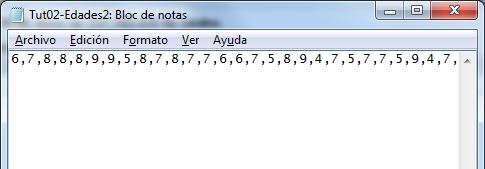
\includegraphics[width=12cm]{../fig/Tut02-07a.png}
    \end{center}
Desde luego, no nos podemos plantear transformar a mano este vector en uno como el anterior. La solución que te proponemos pasa por la hoja de cálculo, y la opción de trasponer una tabla que hemos visto en el Tutorial-00: lo leeríamos en una fila de la hoja, y luego habría que usar el {\tt Pegado especial} para trasponerlo -es decir, girarlo- para finalmente volver a guardarlo. Alternativamente, hay otras soluciones, sin salir de R, usando una función llamada {\tt scan} o usando de nuevo {\tt read.table} y trasponiendo la tabla dentro de R. Esos métodos son sencillos cuando se aprende un poco más sobre R, pero por el momento, y para los ejemplos sencillos que encontraremos, nos vamos a conformar con ese enfoque básico que usa la hoja de Cálculo si es necesario.

\subsection{Cómo obtener ayuda y usar el tabulador en RStudio.}

Vamos a aprovechar estos ejemplos de lectura de ficheros {\tt csv} para aprender a obtener ayuda sobre las funciones de R. La mayoría de las funciones de R, como la función {\tt read.table} o la función {\tt scan} que hemos mencionado al final del anterior apartado, tienen muchos argumentos opcionales. Y hay muchísimas funciones en R (cada vez más, porque, como veremos más adelante, usuarios de todo el mundo añaden constantemente  funciones nuevas a R cuando las necesitan). No es posible recordar todos esas funciones, cada una con sus opciones, así que es muy importante aprender a obtener esa información cuando la necesitamos.

Para ver como obtener esa información en RStudio, vamos a usar por ejemplo la función {\tt scan}. Sitúate en una línea vacía de la Consola de Comandos, escribe {\tt scan} y a continuación, mientras el cursor parpadea junto a la {\tt n} final de {\tt scan}, pulsa la tecla del tabulador (si esto no funciona, usa la tecla {\tt F1} y mira el panel ayuda de RStudio). Verás aparecer una ventana emergente con información sobre la función {\tt scan}, como en esta figura:
    \begin{center}
    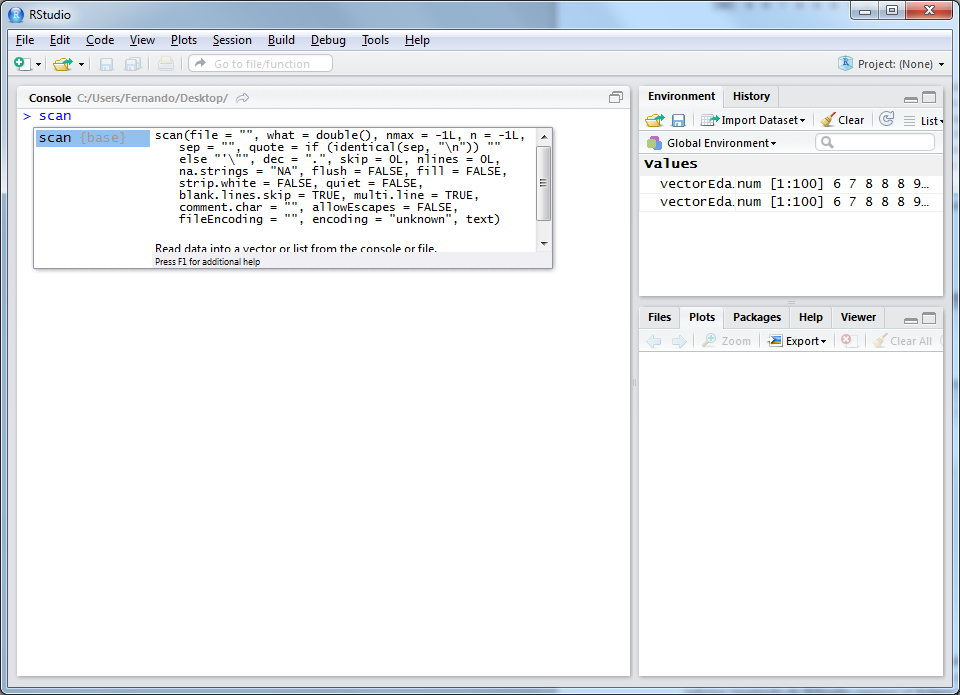
\includegraphics[width=15cm]{../fig/Tut02-08.png}
    \end{center}
Como ves, se muestra un resumen sobre la función {\tt scan}, que a veces será suficiente. Si necesitas más detalles, haz caso a la indicación que aparece al final de esa ventana, y pulsa la tecla {\tt F1}. Al hacerlo, verás que en el panel inferior derecho de RStudio aparece el {\sf fichero de ayuda} de la función {\tt scan}, como en esta figura:
    \begin{center}
    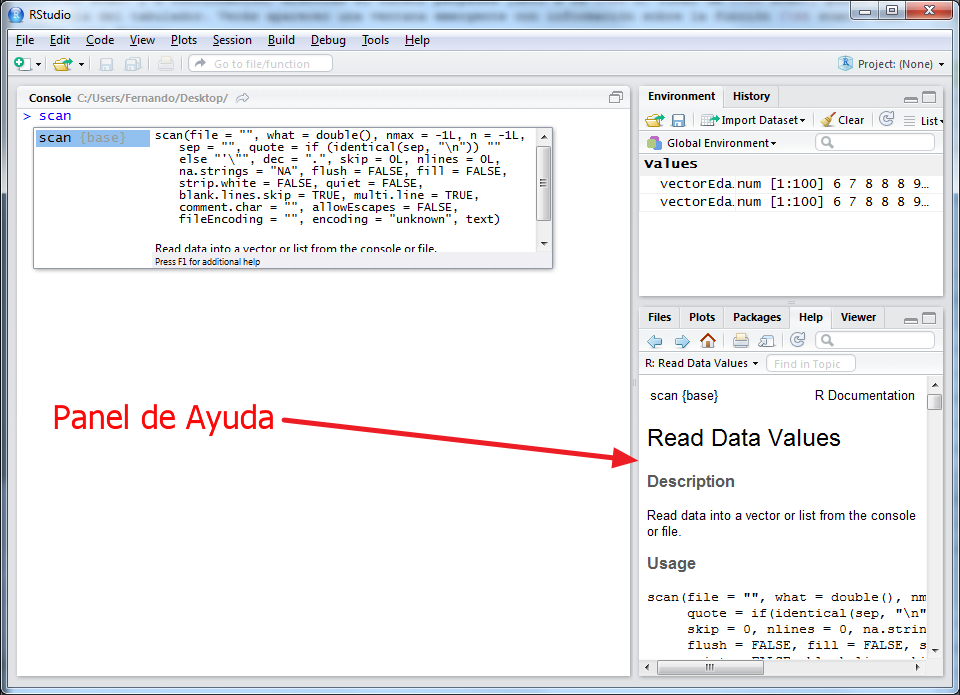
\includegraphics[width=14cm]{../fig/Tut02-09.png}
    \end{center}
Esos ficheros de ayuda son muy útiles, aunque al principio pueden resultar un poco intimidatorios, ya sea por un exceso de información, ya sea porque se da por supuesto que el usuario ya entiende algunos conceptos básicos de R. Podemos garantizar al lector que, a medida que se progresa en R, la utilidad de estos ficheros aumenta.

Pero la utilidad de la tecla tabulador en RStudio no se acaba ahí. Supongamos que quieres aplicar {\tt read.table} para leer el fichero {\tt Tut02-Edades.csv}. Pero te da pereza escribir un nombre tan largo, o no recuerdas exactamente el nombre, o dudas entre dos nombres... no importa cual sea el motivo. Empiezas a escribir la orden, tecleas 
    \begin{center}
    \begin{minipage}{10cm}
    \verb#    (vectorEdades2 = read.table("./datos/ #
    \end{minipage}
    \end{center}
y, de nuevo, justo en este punto pulsas el tabulador. Entonces RStudio te ofrece, en una nueva ventana emergente, todos los ficheros disponibles en la carpeta datos:
    \begin{center}
    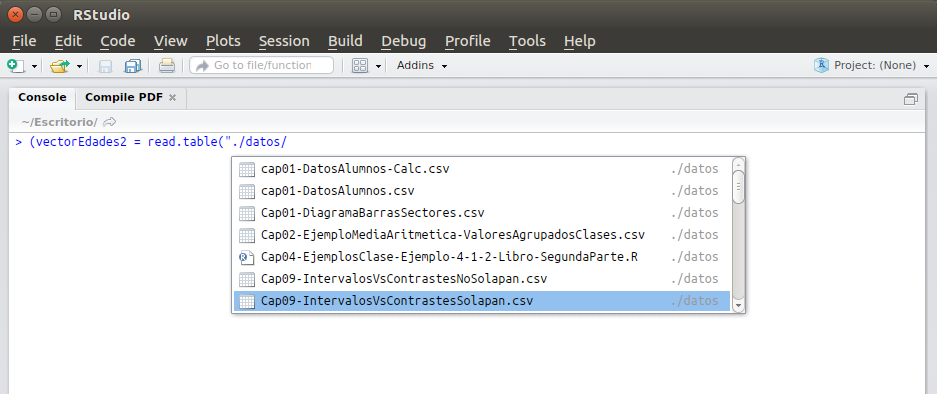
\includegraphics[width=14cm]{../fig/Tut02-11b.png}
    \end{center}
Y ahora puedes usar esa lista seleccionar el fichero que quieras utilizar. Puedes también teclear alguna letra más del nombre para acotar aún más la búsqueda, cuando la carpeta contiene muchos ficheros.


% hemos empezado a usar la función {\tt read.table}, como antes, para cargar el contenido del fichero {\tt Tut02-Edades2.csv} en un vector. Pero nos da olvidado cual era el argumento que nos permitía elegir la coma como separador. No pasa nada, cuando tenemos escrita una parte del comando, como en
%     \begin{center}
%     \begin{minipage}{10cm}
%     \verb#    ( vectorEdades2="../datos/Tut02-Edades2.csv",#
%     \end{minipage}
%     \end{center}
% entonces, después de teclear la coma (sin la coma no funcionará), pulsamos el tabulador y una nueva ventana emergente nos informa de los posibles argumentos que (probablemente) podemos querer usar.
%     \begin{center}
%     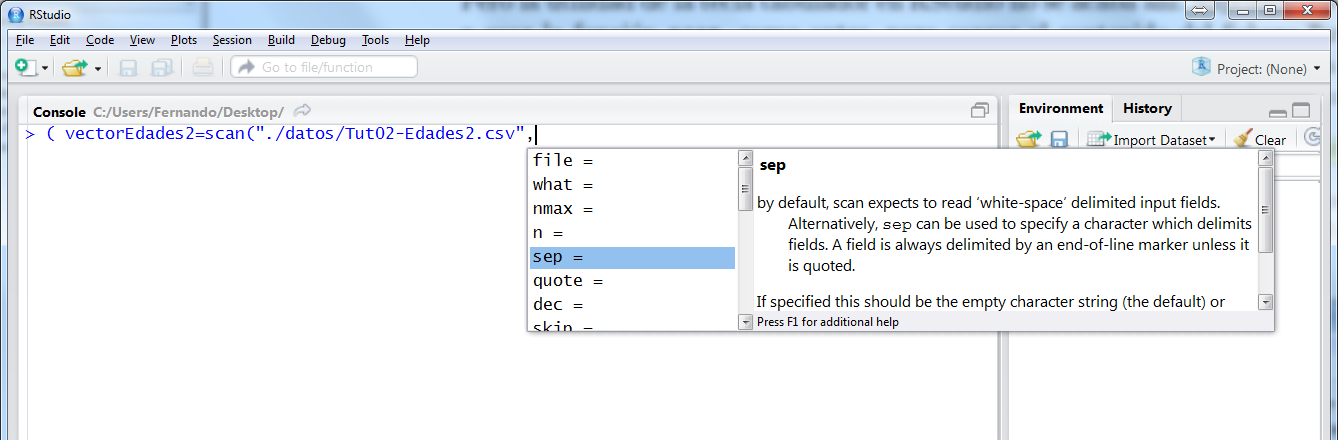
\includegraphics[width=14cm]{../fig/Tut02-10b.png}
%     \end{center}
% Entre ellos (en quinto lugar) aparece {\tt sep}, y al colocar el ratón sobre él, obtenemos de nuevo una explicación más detallada.\\
% Finalmente, para terminar de intentar venderte la idea de que, en RStudio, el tabulador es tu amigo, imagínate que, de nuevo,  

En general, la idea es que en RStudio el tabulador es tu amigo. Como tendremos ocasión de comprobar, RStudio nos ofrece bastante ayuda, para hacer más cómodo nuestro trabajo con R, y el tabulador es una de las herramientas más versátiles y útiles.

\subsection{El camino contrario:  escribir un vector a un fichero de tipo {\tt csv}.}

%Al principio de esta sección (página \pageref{tut03:lugar:vectorEdadesIncrementadas}), después de hacer operaciones con el vector {\tt vectorEdades} hemos fabricado un nuevo –- e interesantísimo –- vector {\tt edadesIncrementadas}, que seguramente querremos guardar para otra sesión, o utilizar en otro programa (por ejemplo una hoja de cálculo, etc.).

Hemos aprendido a leer con R vectores de datos, a partir de ficheros de tipo {\tt csv}. Pero muchas veces, después de hacer operaciones en R, obtendremos como resultados nuevos vectores (y, más adelante en el curso, otro tipo de objetos). Lo natural, entonces,  es aprender a guardar ese vector en un fichero de tipo {\tt csv}, como el fichero con el que empezamos. De esa forma, por ejemplo, puedes compartir tus resultados con otras personas que utilicen programas distintos de R.  Para ello, si antes usábamos la función {\tt read.table}, ahora vamos a usar la función {\tt write.table} de R.\\

Como ejemplo, vamos a utilizar este vector de números enteros.\\

$29$, $ 17$, $ 63$, $ 31$, $ 55$, $ 9$, $ 92$, $ 61$, $ 10$, $ 16$, $ 63$, $ 6$, $ 61$, $ 59$, $ 66$, $ 41$, $ 68$, $ 6$, $ 99$, $ 21$, $ 87$, $ 68$, $ 52$, $ 83$, $ 66$, $ 98$, $ 45$, $ 50$, $ 24$, $ 100$, $ 83$, $ 37$, $ 44$, $ 4$, $ 97$, $ 67$, $ 56$, $ 74$, $ 75$, $ 71$, $ 55$, $ 22$, $ 86$, $ 22$, $ 93$, $ 65$, $ 38$, $ 84$, $ 54$, $ 83$, $ 100$, $ 71$, $ 99$, $ 19$, $ 63$, $ 11$, $ 11$, $ 62$, $ 91$, $ 20$, $ 79$, $ 42$, $ 59$, $ 95$, $ 70$, $ 74$, $ 8$, $ 25$, $ 45$, $ 58$, $ 57$, $ 75$, $ 81$, $ 34$, $ 70$, $ 68$, $ 39$, $ 12$, $ 14$, $ 21$

\begin{ejercicio}
\label{tut02:ejercicio05}
\quad\\
Usa {\em copiar y pegar} a partir de este documento pdf,  para crear un vector de R, llamado {\tt muestra}, que contenga esos datos.
\qed
\end{ejercicio}


Para guardar ese vector {\tt muestra} en un fichero {\tt csv} (dentro de la subcarpeta {\tt datos} del {\em directorio de trabajo}) podemos utilizar la función {\tt write.table}, usando como argumentos:
 \begin{itemize}
   \item El nombre del vector que queremos guardar, que es {\tt muestra}.
   \item Y el nombre del fichero en el que lo guardamos. Vamos llamarlo, por ejemplo, {\tt Tut02-muestra.csv}. Le indicamos a R, además, que lo ponga en la subcarpeta {\tt datos}.
   \item La opción  {\tt col.names = FALSE} o {\tt col.names = TRUE}, para decidir si queremos que R incluya una línea de cabecera con el nombre de la variable, que en este caso es {\tt muestra} (y que no vamos a incluir).
   \item La opción  {\tt row.names = FALSE} para evitar que R incluya números de fila en el fichero de salida (normalmente no querremos esos números).
 \end{itemize}
Es decir, que ejecutamos:
\begin{verbatim}
write.table(muestra,file = "./datos/Tut02-muestra.csv", col.names=FALSE, row.names=FALSE)
\end{verbatim}
%    \begin{center}
%    \begin{minipage}{10cm}
%    \verb#     cat(edadesIncrementadas,file="edadesInc.csv") #
%    \end{minipage}
%    \end{center}
% No obstante, si hacemos esto, R fabricará un fichero en el que los elementos del vector aparecen uno tras otro separados por espacios, como se muestra en la figura (sólo son visibles los primeros valores del vector):
%     \begin{center}
%     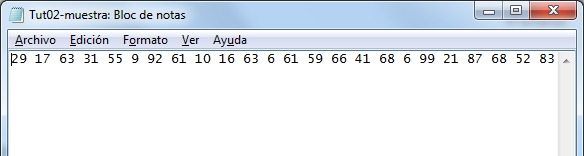
\includegraphics[width=14cm]{../fig/Tut02-12a.png}
%     \end{center}
% Es fácil imaginar que, si lo queremos separado por comas, debemos usar la opción \verb# sep = ","#. Al hacer esto, se obtiene un fichero con este aspecto (en el editor de texto)
%     \begin{center}
%     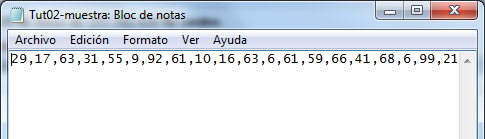
\includegraphics[width=14cm]{../fig/Tut02-13a.png}
%     \end{center}
% que todavía nos puede dar algún problema al tratar de abrirlo en Calc: los datos aparecerán en una fila, y no en una columna. Como hemos dicho antes, esto se puede arreglar dentro del propio Calc. Pero es que hay una solución mucho más fácil, en R, usando la opción {\tt fill} en lugar de {\tt sep}. 
Al ejecutar esa orden  
% \begin{verbatim}
%         cat(muestra,file = "../datos/Tut02-muestra.csv", fill = 1 )
% \end{verbatim}
el fichero que obtenemos tiene la forma deseada (de nuevo, sólo es visible el comienzo del fichero):
    \begin{center}
    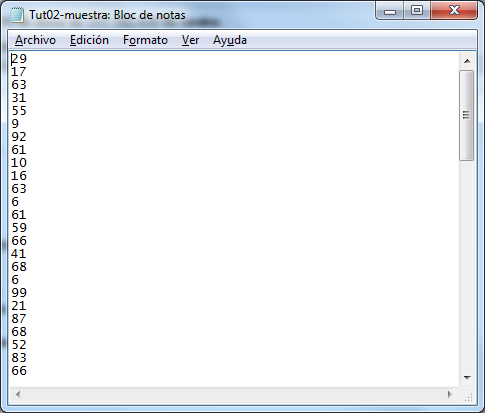
\includegraphics[width=11cm]{../fig/Tut02-14.png}
    \end{center}
Puedes probar a abrirlo en Calc para ver que es un fichero de datos como los que hemos visto hasta ahora.\\

Naturalmente, apenas hemos rozado el tema de la entrada/salida de datos en R. Pero con lo que hemos aprendido en este apartado, estamos listos para empezar a hacer Estadística Descriptiva, usando ejemplos que no sean demasiado triviales.

\section{Estadística descriptiva de una variable cuantitativa, con datos no agrupados.}
\label{tut03:sec:EstadisticaDescriptivaVariableCuantitativaConR}

Para seguir adelante, tenemos que empezar por aprender un poco más sobre la forma en la que R permite operar con los vectores. Vamos a hacerlo a través de una serie de ejercicios-ejemplos.

\begin{ejercicio}
\label{tut02:ejercicio06}
\quad\\
\begin{enumerate}
  \item Vamos a definir dos vectores, cada uno de ellos con $12$ números enteros. El primero, al que llamaremos {\tt vector1}, está formado por:
      \begin{center}
        $8$, $5$, $19$, $9$, $17$, $2$, $28$, $18$, $3$, $4$, $19$, $1$.
      \end{center}
      Usa {\em copiar y pegar} a partir de este fichero pdf para definir el {\tt vector1} en R.

  \item El segundo vector, al que en un rapto de originalidad llamaremos {\tt vector2}, está almacenado en el fichero:
      \begin{center}
        \fichero{../datos/Tut02-vector2.csv}{Tut02-vector2.csv}
      \end{center}
      Guárdalo en {\tt datos} y examínalo primero con un editor de texto (como el {\em Bloc de Notas}), para ver cómo están almacenados los datos en ese fichero. Una vez hecho esto, usa Calc y la función {\tt read.table} para almacenar el contenido de ese fichero csv en  el {\tt vector2} de R. En algún momento del proceso puede que tengas que usar el {\em pegado especial} de {\tt Calc} para trasponer los datos.
\end{enumerate}
Solución en la página \pageref{tut02:ejercicio06:sol}. \qed
\end{ejercicio}

\subsection{Aritmética vectorial en R.}
\label{tut02:subsec:AritmeticaVectorial}

Ahora vamos a sumar los dos vectores. Ejecuta el comando:
        \begin{verbatim}
        vector1 + vector2
        \end{verbatim}
para comprobar que el resultado es la suma, componente a componente, de los dos vectores:
        \begin{verbatim}
            > vector1 + vector2
             [1] 26 23 39 21 37  3 58 24 29 24 34 26
        \end{verbatim}
Este resultado es bastante previsible. Lo que quizá resulté un poco más inesperado es que si multiplicas los dos vectores, también se obtienen los productos componente a componente: el  primer elemento de {\tt vector1} se multiplica por el primero de {\tt vector2}, el segundo por el segundo, etc.:
        \begin{verbatim}
            > vector1 * vector2
             [1] 144  90 380 108 340   2 840 108  78  80 285  25
         \end{verbatim}
Esta forma de operar de R, como veremos pronto, es muy útil. Si lo piensas un momento, cada vector numérico de R se corresponde con una columna de una hoja de cálculo, como las que usábamos en el Tutorial01. Allí vimos que, para algunas operaciones, era necesario multiplicar dos columnas, elemento a elemento. En Calc esa operación no es complicada, pero en R es aún más fácil. Basta con un comando como {\tt vector1 * vector2} para conseguir el objetivo. Veremos muchos más ejemplos, a lo largo del curso, en los que una operación que, en Calc, requeriría bastantes pasos, en R se reduce a ejecutar un único comando.

En R, las operaciones con vectores siguen, en general, este esquema de funcionamiento, componente a componente. Si, por ejemplo, ejecutas
    \begin{verbatim}
    > vector1 + 5
     [1] 13 10 24 14 22  7 33 23  8  9 24  6
    > 2 * vector1
     [1] 16 10 38 18 34  4 56 36  6  8 38  2
    \end{verbatim}
verás que, en el primer caso, cada uno de los elementos de {\tt vector1} se ha incrementado en $5$, mientras que, en el segundo caso, cada uno se ha multiplicado por $2$. Sucede lo mismo con otras operaciones, como elevar al cuadrado:
    \begin{verbatim}
        > vector1^2
         [1]  64  25 361  81 289   4 784 324   9  16 361   1
    \end{verbatim}
Y podemos aplicar funciones en un solo paso. Por ejemplo, podemos calcular el logaritmo neperiano de todos los elementos de un vector en un sólo paso:
    \begin{verbatim}
    > log(vector1)
     [1] 2.0794415 1.6094379 2.9444390 2.1972246 2.8332133 0.6931472
     [7] 3.3322045 2.8903718 1.0986123 1.3862944 2.9444390 0.0000000
    \end{verbatim}
Los resultados de todas estas operaciones son, de nuevo, vectores. Y, por tanto, se pueden asignar a nuevas variables para utilizarlos en nuestras operaciones. Por ejemplo, si luego vas a necesitar los logaritmos de {\tt vector1}, puedes definir una variable para identificar ese vector, llamada {\tt logVector1} (e el nombre que tú quieras), haciendo:
    \begin{verbatim}
    > logVector1 = log(vector1)
    \end{verbatim}
Recuerda que si, además de la asignación, quieres ver el resultado, puedes rodear toda esta sentencia con paréntesis. De lo contrario R la ejecuta, pero no imprime ninguna respuesta, como ya sabes.\\

Aunque al principio puede parecer complicado, cuando te acostumbres a esta forma de trabajar con vectores, verás que resulta muy cómoda y eficiente.

\subsubsection*{Generando vectores de números enteros consecutivos}

Hay muchas ocasiones en que, para alguna operación, necesitamos un vector que contenga los números enteros consecutivos del $1$ al $n$, o del $0$ al $n$, etc. En R esto es muy fácil de hacer. Por ejemplo, para conseguir un vector con los números del $1$ al $15$ basta con ejecutar:
    \begin{verbatim}
    > 1:15
     [1]  1  2  3  4  5  6  7  8  9 10 11 12 13 14 15
    \end{verbatim}
Esa notación con los dos puntos permite generar vectores en los que cada elemento es igual al anterior más $1$. Otro ejemplo:
    \begin{verbatim}
    > -7:13
     [1] -7 -6 -5 -4 -3 -2 -1  0  1  2  3  4  5  6  7  8  9 10 11 12 13
    \end{verbatim}
O incluso, cuando los puntos de partida no son enteros:
    \begin{verbatim}
    > 1.5:7.5
    [1] 1.5 2.5 3.5 4.5 5.5 6.5 7.5
    > 1.5:7.4
    [1] 1.5 2.5 3.5 4.5 5.5 6.5
    \end{verbatim}
¿Ves la diferencia entre estos dos casos?\\

Es muy posible que te estés preguntando ¿y si quiero ir avanzando de $2$ en $2$, o quiero ir hacia atrás (``avanzando'' de $-2$ en $-2$, por ejemplo)? Pronto, cuando hayamos aprendido un poco más, volveremos sobre esto, y comprobaremos que R nos ofrece un catálogo de herramientas extremadamente potentes, para fabricar vectores de acuerdo con nuestros deseos y necesidades.

Los vectores fabricados con este método son vectores iguales que los demás, y se pueden asignar a variables, operar con ellos, etc.

\begin{ejercicio}
\label{tut02:ejercicio07}
\quad\\
\begin{enumerate}
  \item Fabrica un vector con los cuadrados de los números del $1$ al $10$, y asígnalo a la variable {\tt cuadrados}. Usa los paréntesis para ver el resultado de la asignación.
  \item Haz lo mismo con los cuadrados de los números del $2$ al $11$, y un vector {\tt cuadrados2}.
  \item Resta los vectores {\tt cuadrados2 - cuadrados}. ¿Observas algo interesante?
\end{enumerate}
Solución en la página \pageref{tut02:ejercicio07:sol}. \qed
\end{ejercicio}


\subsubsection*{Funciones vectoriales}

Hemos visto antes que se puede aplicar una función, como la raíz cuadrada, a un vector, y se obtiene como resultado otro vector con las raíces cuadradas, elemento a elemento. Pero hay otro tipo de funciones que permiten hacer cálculos con el vector {\em en conjunto}. Por ejemplo, antes hemos fabricado el vector {\tt -7:13}, y la función {\tt length} nos dice cuantos elementos tiene ese vector:
    \begin{verbatim}
    > length(-7:13)
    [1] 21
    \end{verbatim}
En el Ejercicio \ref{tut02:ejercicio03} (pág. \pageref{tut02:ejercicio03}) nos preguntábamos cuantos elementos tenía el vector {\tt vectorEdades} que habíamos cargado desde el fichero {\tt csv}. Puedes obtener la respuesta con {\tt length(vectorEdades)}. Para comprobarlo, asegúrate de que has creado el vector llamado {\tt vectorEdades} y ejecuta esta orden:
\begin{center}
\begin{tabular}{l}
{\tt > length(vectorEdades) }\\
{\tt [1] 100 }
\end{tabular}
\end{center}
Como ves, el resultado de {\tt length} es el esperado. \\

Vamos a conocer otra función, llamada {\tt sum}, que sirve para calcular la suma de todos los elementos de un vector:
\begin{verbatim}
> sum(vectorEdades)
[1] 675
\end{verbatim}

\begin{ejercicio}
\label{tut02:ejercicio08}
\quad\\
¿Cuánto vale la suma de los cuadrados de los números del $1$ al $100$?
Solución en la página \pageref{tut02:ejercicio08:sol}. \qed
\end{ejercicio}

\paragraph*{}\label{tut02:lugar:CalculoManualMediaAritmetica} A lo mejor te ha pasado desapercibido, pero con las funciones {\tt length} y {\tt sum} estamos, por fin, en condiciones de empezar a hacer Estadística Descriptiva. Por ejemplo, podemos calcular la media aritmética de {\tt vectorEdades}:
\begin{verbatim}
> ( mediaEdades = sum(vectorEdades) / length(vectorEdades) )
[1] 6.75
\end{verbatim}
Y una vez que tenemos la media, podemos calcular la varianza poblacional. Para que resulte más claro, vamos a mostrarte el proceso paso a paso, aunque al final lo ejecutaremos en un sólo paso:
\begin{enumerate}
  \item Empezamos restando la media, que está en la variable {\tt mediaEdades}, de cada uno de los elementos de {\tt vectorEdades}:
    \begin{verbatim}
    vectorEdades - mediaEdades
    \end{verbatim}
      El resultado es un {\em vector de diferencias}.
  \item Ahora elevamos cada una de esas diferencias al cuadrado:
    \begin{verbatim}
    ( vectorEdades - mediaEdades )^2
    \end{verbatim}
    El resultado de este paso es, de nuevo, un {\em vector}, ahora con las diferencias al cuadrado. Fíjate en el paréntesis, para garantizar que elevamos al cuadrado la diferencia. Si no incluyéramos el paréntesis ¿qué calcularíamos?
  \item A continuación sumamos todas esas diferencias al cuadrado, usando la función {\tt sum}:
    \begin{verbatim}
    sum( ( vectorEdades - mediaEdades )^2)
    \end{verbatim}
    De nuevo, el paréntesis es fundamental, para que el cuadrado del vector de diferencias se calcule antes que la suma. En este paso, el resultado ya no es un vector, sino un {\em número}.
  \item Por último, dividimos esa suma por $n$, el número de elementos de {\tt vectorEdades}, que se obtiene con la función {\tt length}:
    \begin{verbatim}
    sum( ( vectorEdades - mediaEdades )^2) / length(vectorEdades)
    \end{verbatim}
\end{enumerate}
El resultado de estos pasos se puede condensar en un sólo comando de R, en el que a la vez calculamos la varianza y la asignamos a una variable:
        \begin{verbatim}
    > ( varEdades = sum( ( vectorEdades - mediaEdades )^2) / length(vectorEdades) )
    [1] 1.9875
        \end{verbatim}

\begin{ejercicio}
\label{tut02:ejercicio09}
\quad\\
\begin{enumerate}
  \item Calcula la desviación típica (poblacional) de {\tt vectorEdades}.
  \item Calcula la cuasivarianza y cuasidesviación típica (muestrales) de {\tt vectorEdades}.
  \item ¿Qué sucede si en el tercer paso ejecutas el siguiente comando?\\
    {\centering\verb#sum(  vectorEdades - mediaEdades )^2#}\\
  ¿Por qué sucede esto?
\end{enumerate}
Solución en la página \pageref{tut02:ejercicio09:sol}.  \qed
\end{ejercicio}

Con estos cálculos hemos empezado a hacer Estadística con R. Naturalmente, nos queda muchísimo que aprender sobre los vectores de R. Por ejemplo, como se accede a una componente individual del vector, para responder a preguntas como {\em ``¿Cuánto vale el quinto elemento del vector?''} Más en general, aprenderemos a extraer aquellos elementos del vector que cumplan alguna condición, respondiendo a preguntas como {\em ``¿Qué elementos del vector son mayores que $7$?''}

\subsection{Y, por fin, hagamos Estadística Descriptiva.}
\label{tut02:subsec:PorFinHagamosEstadisticaDescriptiva}

En esta sección vamos a trabajar con un vector de datos contenido en este fichero adjunto:
\begin{center}
  \fichero{../datos/Tut02-var3.csv}{Tut02-var3.csv}
\end{center}
Este vector contiene los datos de la variable {\tt var3} del fichero {\tt Tut01-PracticaConCalc.csv}, que ya hemos utilizado en el Tutorial-00 para aprender a hacer Estadística Descriptiva con Calc. En esta sección vamos a reproducir los resultados que obtuvimos allí, pero esta vez usando R. Para preparar el terreno vamos a hacer limpieza.
\begin{ejercicio}
\label{tut02:ejercicio10}
\quad\\
\begin{enumerate}
  \item Cierra Rstudio y vuelve a abrirlo, para limpiar la memora del sistema. El trabajo que hemos hecho hasta ahora se perderá (aunque los comandos siguen en el Historial de Comandos que ya vimos).
  \item Establece el {\em Directorio de Trabajo} (por ejemplo, el {\em Escritorio}), y asegúrate de que {\tt Tut02-var3.csv} está guardado en la subcarpeta {\tt datos} de ese directorio.
  \item Carga de nuevo el contenido de ese fichero en un vector {\tt var3} de R.
\end{enumerate}
Solución en la página \pageref{tut02:ejercicio10:sol}.  \qed
\end{ejercicio}

Verás, en lo que sigue, que siempre que calculamos un objeto le asignamos una variable. Eso permite ahorrarse la repetición innecesaria de cálculos, si más adelante volvemos a necesitar ese objeto. Y en algunos casos, como veremos más adelante, al hacer esto podemos acceder a propiedades del objeto calculado que R no muestra en su respuesta por defecto.

\subsubsection*{Rango, máximo y mínimo.}

Para empezar, vamos a aprender tres nuevas funciones de R que nos permiten calcular esos tres valores:

        \begin{verbatim}
        > (minimo = min(var3) )
        [1] 0
        > (maximo = max(var3) )
        [1] 16
        > (rango = range(var3) )
        [1]  0 16
        \end{verbatim}
El funcionamiento de las dos primeras es evidente. La función {\tt range} devuelve un {\em vector}, formado por el máximo y el mínimo.

\subsubsection*{Tablas de frecuencia. Clases de objetos en R}

La tabla de frecuencia absoluta de {\tt var3} se obtiene usando la función {\tt table}, de esta forma tan sencilla:

    \begin{verbatim}
    > ( tablaFrecAbs = table(var3) )
    var3
      0   1   2   3   4   5   6   7   8   9  10  11  12  13  14  16
      9  25 100 188 244 246 186 131  87  43  28   6   2   2   2   1
    \end{verbatim}
La primera fila contiene los elementos de {\tt var3}, y en la segunda aparece la frecuencia de cada uno de ellos. Puedes comprobar que son los mismos resultados que obtuvimos, con Calc, en la página \pageref{tut01-tut01:lugar:TablaFrecuenciasVar3} del Tutorial01. Aunque allí, desde luego, el proceso fue más laborioso.\\

A lo mejor te has dado cuenta de que el formato de la respuesta es diferente de los que hemos obtenido hasta ahora. Para empezar, la respuesta no empieza con el {\tt [1]} al que  ya nos vamos acostumbrando. El motivo de esto es que el objeto que hemos obtenido como respuesta no es un vector, sino una tabla. Ya dijimos que R utiliza distintos tipos de objetos, con fines distintos. ¿Cómo podemos saber de qué clase es un objeto? Pues usando una función de R, oportunamente llamada {\tt class}. Si la usamos con el vector {\tt var3} y con su tabla de frecuencias, obtenemos:
    \begin{verbatim}
    > class(var3)
    [1] "numeric"
    > class(tablaFrecAbs)
    [1] "table"
    \end{verbatim}
El vector {\tt var3} es de clase {\tt numeric} porque es un vector de números. Y la tabla de frecuencias es de clase {\tt table}. Veremos a lo largo del curso otros objetos de tipo {\em tabular}, como las matrices (clase {\tt matrix}), los conjuntos de datos (clase {\tt data.frame}) y los {\tt arrays}.

Aunque las tablas son objetos distintos de los vectores, tienen algunas propiedades en común, y algunas de las funciones que hemos usado con vectores también se pueden usar con tablas.

\begin{ejercicio}
\label{tut02:ejercicio11}
\quad\\
Aplica las funciones {\tt length}, {\tt sum}, {\tt min}, {\tt max} y {\tt range} a la tabla {\tt tablaFrecAbs}. Solución en la página \pageref{tut02:ejercicio11:sol}.
\qed
\end{ejercicio}
Siguiendo con los parecidos entre tablas y vectores, puedes multiplicar (o dividir) una tabla por un número, y la operación se hará elemento a elemento:
    \begin{verbatim}
    > 2 * tablaFrecAbs
    var3
      0   1   2   3   4   5   6   7   8   9  10  11  12  13  14  16
     18  50 200 376 488 492 372 262 174  86  56  12   4   4   4   2
    \end{verbatim}
Como ves, cada frecuencia se multiplica por $2$. Esta propiedad de las tablas permite obtener, de forma, muy sencilla la tabla de frecuencias relativa de {\tt var3}. Como primer paso, vamos a guardar la longitud de {\tt var3} en la variable {\tt n}:
    \begin{verbatim}
    > ( n = length( var3 ) )
    [1] 1300
    \end{verbatim}
Y ahora podemos dividir la tabla por {\tt n} para conseguir la tabla de frecuencias relativas (hemos estrechado la {\em Consola de Comandos} para que el resultado cupiera en esta página).
    \begin{verbatim}
    > ( tablaFrecRel = tablaFrecAbs / n )
    var3
               0            1            2            3            4
    0.0069230769 0.0192307692 0.0769230769 0.1446153846 0.1876923077
               5            6            7            8            9
    0.1892307692 0.1430769231 0.1007692308 0.0669230769 0.0330769231
              10           11           12           13           14
    0.0215384615 0.0046153846 0.0015384615 0.0015384615 0.0015384615
              16
    0.0007692308
    \end{verbatim}
\begin{ejercicio}
\label{tut02:ejercicio12}
\quad\\
Ya sabemos cuanto debe sumar esta tabla de frecuencias relativas. Compruébalo. Solución en la página \pageref{tut02:ejercicio12:sol}.
\qed
\end{ejercicio}

Si lo que queremos es una tabla de frecuencias acumuladas, debemos emplear la función {\tt cumsum}.

\begin{verbatim}
> ( tablaFrecAcu = cumsum(tablaFrecAbs)  )
   0    1    2    3    4    5    6    7    8    9   10   11   12   13   14   16
   9   34  134  322  566  812  998 1129 1216 1259 1287 1293 1295 1297 1299 1300
\end{verbatim}

\begin{ejercicio}
\label{tut02:ejercicio13}
\quad\\
La última tabla que falta es la de frecuencias relativas acumuladas, pero ya tienes todos los ingredientes para obtenerla, de dos maneras diferentes. Hazlo, y comprueba si dan el mismo resultado.  Si no es así, ¿a qué crees que se debe, y cuál es la mejor opción? Asigna el resultado a la variable {\tt tablaFrecRelAcu}.
Solución en la página \pageref{tut02:ejercicio13:sol}.  \qed
\end{ejercicio}

\subsubsection*{Gráficos de columnas y diagramas de caja (boxplot). Argumentos con nombre.}

Vamos a fabricar nuestros primeros gráficos con R. En concreto, vamos a dibujar un gráfico de barras a partir de la tabla de frecuencias de {\tt var3}, usando la función {\tt barplot} de R:
\begin{verbatim}
> barplot(tablaFrecAbs)
\end{verbatim}
Al ejecutar este comando no debes ver ninguna salida en la {\tt Consola de Comandos}. En su lugar, en el panel inferior derecho de RStudio, concretamente en la ventana {\em Plots}, aparecerá el gráfico deseado. El resultado puede variar, dependiendo de la anchura de tu ventana de RStudio.
    \begin{center}
    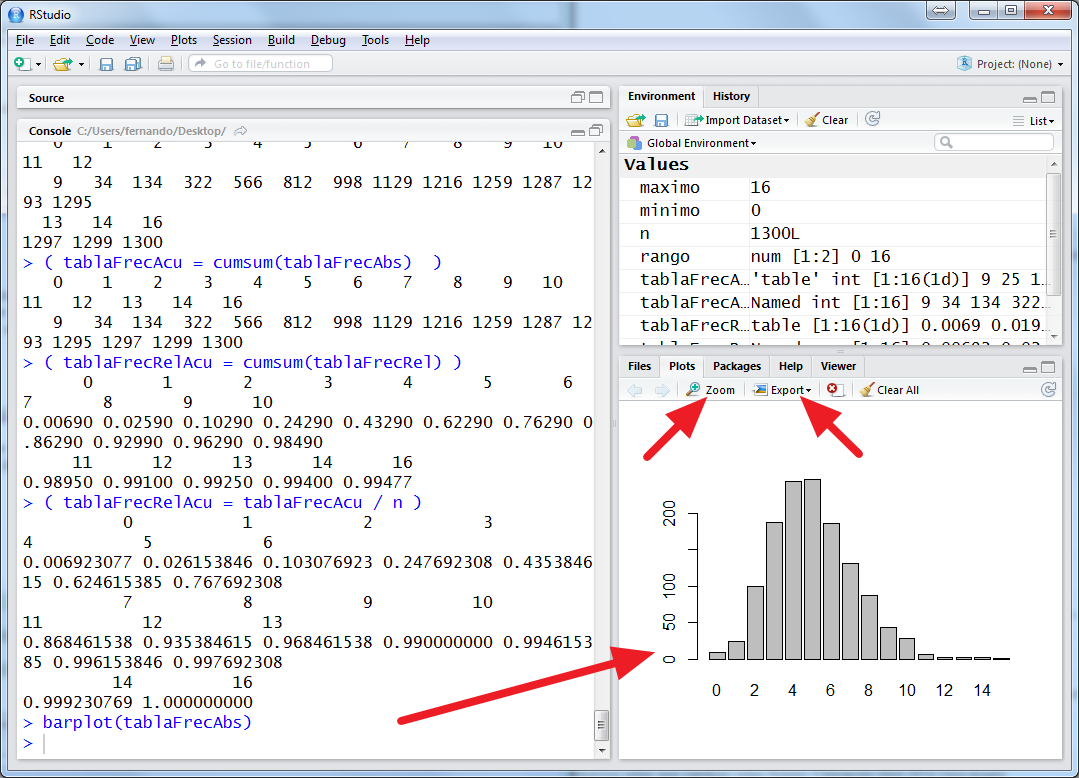
\includegraphics[width=12cm]{../fig/Tut02-15a.png}
    \end{center}

Hemos destacado además, en la figura, los dos botones {\em Zoom} y {\em Export} que te permiten, respectivamente, ver una versión ampliada de la Figura (que se redimensiona dinámicamente si cambias  la ventana), y guardar esa figura como un fichero de gráficos que puedes insertar en cualquier documento, editar con un programa de manipulación de gráficos, etcétera.

Los gráficos de R se pueden controlar hasta en sus detalles más mínimos. Como aperitivo mínimo, vamos a añadir algo de color al gráfico:
\begin{verbatim}
    >  barplot(tablaFrecAbs, col = heat.colors(15))
\end{verbatim}
El resultado es esta figura:
    \begin{center}
    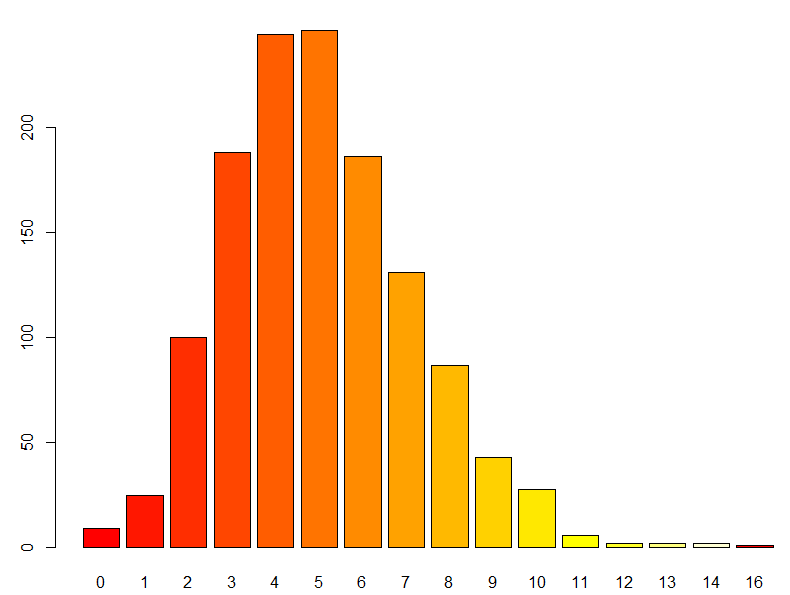
\includegraphics[width=12cm]{../fig/Tut02-16.png}
    \end{center}
Las posibilidades de control de los gráficos de R son, como decimos, inmensas y pueden llegar a ser abrumadoras. Hay libros, de cientos de páginas,  dedicados a este tema, como el {\em R Graphics Cookbook} de W. Chang (ver las referencias del curso). Nosotros, a lo largo de los tutoriales del curso, vamos a aprender algo más, aunque a penas nos podremos limitar a rozar la superficie de lo que se puede llegar a hacer.

En la Sección \ref{curso-cap02:subsubsec:RangoIntercuartilico} del libro hemos descrito los diagramas de cajas, o boxplots (recuerda la Figura \ref{curso-cap02:fig:Boxplot}, de la pág. \pageref{curso-cap02:fig:Boxplot} del libro). Y en el Tutorial-01 dijimos que con Calc no es fácil dibujar ese tipo de diagramas. En cambio, con R, no podría ser más fácil:
\begin{verbatim}
  > boxplot(var3)
\end{verbatim}
Y el resultado es esta figura:
\begin{center}
  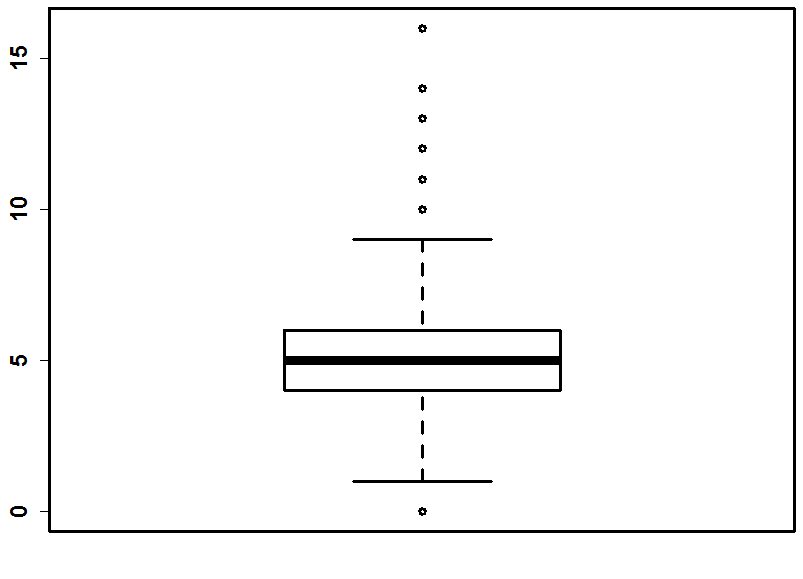
\includegraphics[width=10cm]{../fig/Tut02-17.png}
\end{center}

En realidad tenemos que confesar que el resultado es ligeramente distinto, y que hemos manipulado algunos de los parámetros gráficos de R, para que las líneas fueran más gruesas, y figura resultara más fácil de visualizar. Ya aprenderemos esos trucos. Por el momento, nos limitamos a insistir en lo fácil que resulta obtener el diagrama en R.

Si deseas que la orientación del diagrama sea horizontal, basta con ejecutar
\begin{verbatim}
    boxplot(var3, horizontal=TRUE)
\end{verbatim}
y también puedes controlar si se incluyen, o no, los valores atípicos ({\em outliers}), con el argumento {\tt outline}. Para excluirlos, ejecutaríamos
\begin{verbatim}
    boxplot(var3, outline = FALSE)
\end{verbatim}
Una advertencia: en este, como en otros casos, aunque lo estamos presentando por separado, siempre puedes combinar a la vez varios argumentos opcionales. Por ejemplo, no hay problema en ejecutar:
\begin{verbatim}
    boxplot(var3, horizontal = TRUE, outline = FALSE)
\end{verbatim}
El único problema que puedes tener es el {\em orden} en que colocas esos argumentos opcionales. Por ejemplo, si ejecutas:
\begin{verbatim}
    boxplot(var3, TRUE, FALSE)
\end{verbatim}
entonces R tendrá que decidir por su cuenta (aplicando las reglas que, en su momento, decidieron los programadores), a cuál de sus argumentos opcionales corresponde esos valores {\tt TRUE} y {\tt FALSE}. ¡Y esos argumentos opcionales son muchos, así que el resultado puede ser muy distinto de lo que esperábamos!
\begin{ejercicio}
\label{tut02:ejercicio14}
\quad\\
Ejecuta ese comando para ver el gráfico resultante. Solución en la página \pageref{tut02:ejercicio14:sol}.  \qed
\end{ejercicio}
Para evitar ese problema, R utiliza los {\em argumentos con nombre}, como en {\tt horizontal = TRUE}. Aquí, {\tt horizontal} es el nombre del argumento, y {\tt TRUE} es el valor que le hemos asignado al llamar a la función {\tt boxplot}. Gracias a este mecanismo, podemos conseguir que el orden de los argumentos sea irrelevante.
\begin{ejercicio}
\label{tut02:ejercicio15}
\quad\\
Ejecuta de nuevo el comando:
\begin{verbatim}
    boxplot(var3, horizontal = TRUE, outline = FALSE)
\end{verbatim}
Y ahora, con los argumentos opcionales intercambiados de posición:
\begin{verbatim}
    boxplot(var3, outline = FALSE, horizontal = TRUE)
\end{verbatim}
Verás que no hay ninguna diferencia. Solución en la página \pageref{tut02:ejercicio15:sol}.
\qed
\end{ejercicio}

Para completar, por el momento, la discusión sobre gráficos elementales, queremos comentar que también se pueden dibujar diagramas de sectores en R. Pero vamos a ser consecuentes con nuestra recomendación de no utilizar ese tipo de gráficos, y no incluiremos instrucciones. Siempre puedes buscar en Internet, si realmente quieres dibujarlos.

\subsubsection*{Histogramas en R}
\label{tut02:subsubsec:HistogramasR}

En el Tutorial-01 dijimos que no es fácil usar Calc para dibujar histogramas, y nos comprometimos a mostrar la forma de dibujar ese tipo de gráficos con R. Todavía no estamos en condiciones de aprovecharlos al máximo, porque no hemos visto las herramientas que R nos proporciona para agrupar una variable en clases, y para trabajar después con esas clases. Veremos todo eso más adelante, pero para adelantar algo, vamos a usar la variable {\tt var3}, para comprobar lo fácil que es obtener su histograma, usando el comando:
\begin{verbatim}
    hist(var3, col = heat.colors(15))
\end{verbatim}
El argumento {\tt , col = heat.colors(15)} es opcional, y sólo sirve para fijar la misma combinación de colores que ya usamos en el diagrama de barras. Como en otros casos, hemos manipulado ligeramente el comando para que las líneas sean más gruesas y la visualización sea más fácil. Tú obtendrás un trazo más tenue; ya aprenderemos a hacer ese tipo de ajustes):

\begin{center}
  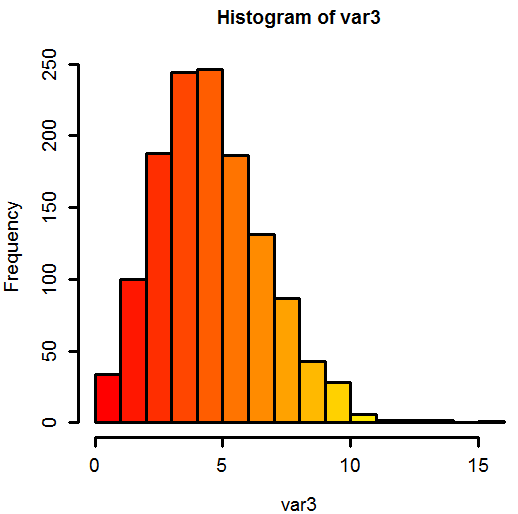
\includegraphics[width=12cm]{../fig/Tut02-59.png}
\end{center}

Como puedes ver, en este caso tan sencillo la información que transmiten el diagrama de barras y el histograma es, esencialmente, la misma. Fíjate en el detalle técnico de que, en el histograma, no existe la separación entre las barras que sí se daba en el otro diagrama. Veremos más adelante ejemplos en los que la diferencia ente ambos tipos de gráficos será mucho más marcada.

\subsubsection*{Media aritmética.}
\label{tut02:subsubsec:MediaAritmetica}

Al final de la Sección \ref{tut02:subsec:AritmeticaVectorial} hemos visto como calcular la media aritmética y la varianza del vector {\tt vectorEdades} {\em ``a mano''}, usando la aritmética vectorial. Pero, desde luego, esas operaciones son tan básicas, que, como sucedía en Calc, es de esperar que R incluya funciones para calcularlas en un paso.

Así, si queremos calcular la media aritmética de {\tt var3}, basta con usar la función {\tt mean}:
    \begin{verbatim}
    > (media = mean(var3))
    [1] 5.039231
    \end{verbatim}

\begin{ejercicio}
\label{tut02:ejercicio16}
\quad\\
\begin{enumerate}
  \item Asegúrate de tener disponible en R el {\tt vectorEdades}, y calcula su media, usando la función {\tt mean}.  Compárala con la que obtuvimos en la página \pageref{tut02:lugar:CalculoManualMediaAritmetica}.
  \item Y a la inversa, calcula la media de {\tt var3} usando aritmética vectorial, sin recurrir a {\tt meam}.
\end{enumerate}
Solución en la página \pageref{tut02:ejercicio16:sol}.  \qed
\end{ejercicio}

\subsubsection*{Cuasivarianza, y cuasidesviación típica. Varianza y desviación típica.}

Con la varianza y la desviación típica, no obstante, tenemos una pequeña dificultad. Los creadores de R diseñaron el programa para hacer Estadística, no para enseñarla. Aunque las cosas han cambiado mucho desde entonces, y ahora R se usa como herramienta de enseñanza en cientos de cursos en todo el mundo, no hay que olvidar que R es, ante todo, una herramienta profesional, y ese espíritu lo  impregna todo.  En particular, como veremos más adelante en el curso, en Estadística, la varianza y desviación típica poblacionales juegan un papel muy secundario, comparado con el de la cuasivarianza y cuasidesviación típica muestrales. La razón es que el trabajo se hace, casi siempre, con muestras, claro. Las cantidades poblacionales son, a menudo, objetos teóricos, esencialmente inaccesibles.

Por esas razones, R no incluye funciones para calcular ni la varianza poblacional, ni la desviación típica poblacional. Sí se  incluyen, en cambio, la función {\tt var} para calcular la cuasivarianza muestral:
\begin{verbatim}
    > (varMuestral = var(var3))
    [1] 4.715165
\end{verbatim}
y la función {\tt sd} para calcular la cuasidesviación típica muestral (que es la raíz cuadrad de la anterior):
\begin{verbatim}
  > (desvTipMuestral = sd(var3))
[1] 2.171443
\end{verbatim}

\begin{ejercicio}
\label{tut02:ejercicio17}
\quad\\
Comprueba que {\tt sd(var3)} es la raíz cuadrada de {\tt var(var3)}. Solución en la página \pageref{tut02:ejercicio17:sol}.
\qed
\end{ejercicio}

¿Y si queremos calcular las cantidades poblacionales? En tal caso, basta con tener en cuenta las definiciones, y para la varianza poblacional hacemos:
\begin{verbatim}
      > ( varPobl= ( (n-1) / n ) * varMuestral )
    [1] 4.711538
\end{verbatim}
y entonces, para la desviación típica poblacional sólo hay que calcular la raíz cuadrada:
\begin{verbatim}
    > ( desvTipPobl = sqrt( varPobl ) )
    [1] 2.170608
\end{verbatim}


\subsubsection*{Medidas de posición: mediana, cuartiles y percentiles. Rango intercuartílico.}

Para calcular la mediana, tenemos la función {\tt median}:
\begin{verbatim}
    > ( mediana = median(var3))
    [1] 5
\end{verbatim}

El cálculo de los cuartiles (o percentiles) en R, como en cualquier otro programa estadístico, requiere una discusión más detallada. Por un lado, si lo único que se desea es obtener la información por defecto que proporciona R, dejando que sea el programa el que decida la mejor forma de proceder, entonces las cosas son muy sencillas. Basta con usar la función {\tt summary}, así:
\begin{verbatim}
  > summary(var3)
   Min. 1st Qu.  Median    Mean 3rd Qu.    Max.
  0.000   4.000   5.000   5.039   6.000  16.000
\end{verbatim}
Como ves, la respuesta incluye varias de las cantidades que ya habíamos calculado previamente, pero también aparecen los cuartiles primero y tercero (indicados por {\tt 1st Qu.} y {\tt 3rd Qu.}, respectivamente).

Esta función {\tt summary} no sólo sirve para vectores, sino que se puede aplicar a muchos otros objetos de R, para obtener (lo que R considera) información básica sobre ellos.

\begin{ejercicio}
\label{tut02:ejercicio18}
\quad\\
¿Qué tipo de objeto produce {\tt summary} en su respuesta? ¿Es una tabla, un vector, otra cosa? Solución en la página \pageref{tut02:ejercicio18:sol}.
\qed
\end{ejercicio}

Además de {\tt summary}, en R disponemos de la función {\tt IQR} para calcular el rango intercuartílico de un vector:
\begin{verbatim}
    > IQR(var3)
    [1] 2
\end{verbatim}
Puedes comprobar que la respuesta es la diferencia entre los dos cuartiles que hemos obtenido con {\tt summary}.\\

Por otra parte, en lugar de utilizar {\tt summary}, si sólo queremos uno de los cuantiles, o si lo que queremos son algunos percentiles, podemos conseguir un control más fino de la respuesta utilizando la función {\tt quantile}. Si la aplicamos al vector, sin más, se obtiene por defecto esta respuesta:
\begin{verbatim}
    > quantile(var3)
      0%  25%  50%  75% 100%
       0    4    5    6   16
\end{verbatim}
Pero también podemos usarla con un segundo argumento: un vector en el que aparecen los porcentajes (expresados como tantos por uno) de los percentiles que queremos calcular. Por ejemplo, para pedirle a R que calcule (con el método por defecto, es decir, el que más le gusta a R) los percentiles 5\%, 15\% y 75\% de {\tt var3}, ejecutamos este comando:
\begin{verbatim}
    > quantile(var3, c(0.05,0.15,0.75))
     5% 15% 75%
      2   3   6
\end{verbatim}
Aquí, como queremos mantener la discusión lo más simple posible, no vamos a entrar en más detalles técnicos sobre las decisiones que R toma para calcular estos números, pero queremos prevenir al lector de que las cosas se complican enseguida: en R hay varias (concretamente, nueve) formas distintas de calcular los cuartiles.


\section{Ficheros de comandos R. Comentarios.}
\label{tut02:sec:FicherosComandosComentarios}

Antes de seguir adelante, tenemos que ocuparnos de un problema que, casi con seguridad, está empezando a preocuparte. Si has hecho todo el trabajo de la sección anterior, habrá escrito muchos comandos de R, para estudiar el vector {\tt var3}. Pero imagínate que ahora queremos estudiar otro vector, por ejemplo, el {\tt vectorEdades} de las primeras secciones de este tutorial. ¿Tenemos que empezar de nuevo, tecleando todos esos comandos para este nuevo vector? Ya sabes que esas instrucciones están guardadas en el {\em Historial de Comandos} (¡incluso las erróneas!). Una opción sería irlas copiando, una por una, desde ese historial a la {\em Consola de Comandos}, modificarlas, y ejecutarlas. Pero no parece una gran idea, en términos de productividad.

La solución es bastante sencilla, y RStudio nos ofrece todo lo que necesitamos. Lo que vamos a hacer es guardar, en un fichero de texto plano, una lista de instrucciones de R.  Esos ficheros de instrucciones tendrán la extensión
\begin{center}
  {\tt.R}
\end{center}
Ya sabes que, como vimos en el Tutorial-01, la extensión sirve para identificar el tipo de fichero, y para decidir cuál es el programa predeterminado con el que el sistema abre esos  ficheros (por ejemplo, al hacer doble clic sobre uno de ellos). Antes de avanzar más, veamos un ejemplo. Pero primero una advertencia, para evitar problemas: \textcolor{red}{\bf\large ¡Lee el siguiente fragmento, entre las líneas horizontales, antes de tratar de abrir el fichero de instrucciones!}\\

\hrule
\hrule
\quad\\
Cierra RStudio antes de empezar, para hacer un poco de limpieza. Hemos creado uno de esos ficheros de instrucciones,  muy sencillo, que puedes  abrir con un editor de texto (como el {\em Bloc de Notas} de Windows):
\begin{center}
  \fichero{./code/Tut02-codigo01.R}{Tut02-codigo01.R},
\end{center}
El contenido, al abrirlo con el editor es este:
    \begin{center}
    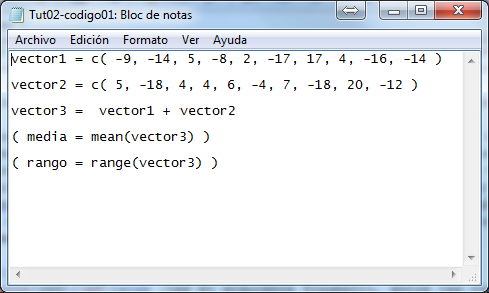
\includegraphics[height=6cm]{../fig/Tut02-18.png}
    \end{center}
Si el ordenador en el que estás trabajando tiene instalado RStudio, como se vio en el Tutorial-00, es muy posible que el programa predeterminado para abrir los ficheros como este sea el propio RStudio. En cualquier caso, para asegurarnos, guarda este fichero en tu ordenador. ¡Recuerda usar el botón derecho para guardar! Además, es importante que lo guardes en el {\em Directorio de Trabajo}. {\bf Atención:} no se trata de guardarlo en la subcarpeta {\tt datos}, sino en el propio directorio de trabajo que contiene esa subcarpeta. Una vez guardado, usa lo que aprendimos en el Tutorial-00 para asegurarte de que, en efecto, RStudio es el programa predeterminado de tu sistema para este tipo de ficheros.\\

Y ahora, después de todas las maniobras anteriores, vamos a abrir el fichero con RStudio.  Puedes hacer doble clic en el fichero, o si prefieres un poco más de control sobre el proceso, puedes empezar abriendo RStudio. En ese caso, usa los menús {\tt File} $\to$ {\tt Open File}, y en la ventana que aparece, selecciona el fichero {\tt Tut02-codigo01.R}, y pulsa en {\tt Abrir}.

\hrule
\hrule
\quad\\

Al abrir el fichero, se abrirá una componente nueva de RStudio, que hasta ahora no habíamos utilizado. Se trata de un nuevo panel de RStudio,  al que vamos a llamar el  {\em Editor de Código} (en inglés, {\em Source Editor}), que se sitúa en la parte superior izquierda de la interfaz, justo encima de la {\em Consola de Comandos}. En ese panel aparece el contenido del fichero {\tt Tut02-codigo01.R},como se ve en la figura:\\

    \begin{center}
    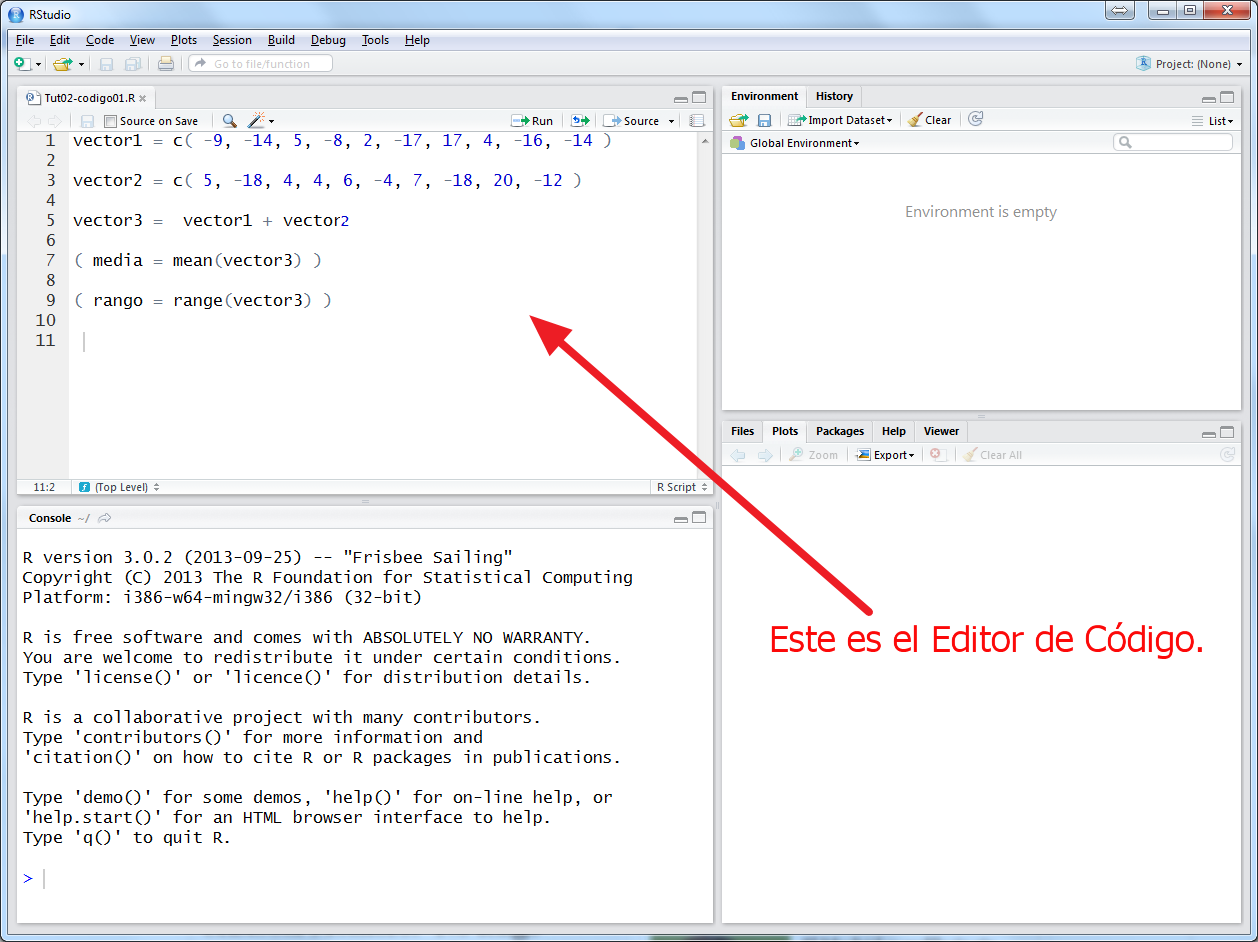
\includegraphics[height=11cm]{../fig/Tut02-19a.png}
    \end{center}

\quad\\
Este {\em Editor de Código} es, ante todo y como indica su nombre, un editor de texto. Es, por así decirlo, como si RStudio llevará incorporado su propio {\em Bloc de Notas}. Pero es, además, y como iremos viendo a lo largo del curso, un editor de texto especialmente diseñado para el trabajo con R. Habrás notado ya que, por ejemplo, se utilizan distintos colores para algunos elementos del ficheros. Además las líneas aparecen numeradas a la izquierda. Todos esos ingredientes, y muchos otros que conoceremos más adelante, están ahí para hacer nuestro trabajo con R mucho más productivo.

Para empezar, vamos a descubrir la relación que existe entre el {\em Editor de Código} y la {\em Consola de Comandos}, que hemos venido usando hasta ahora. Haz clic con el botón izquierdo del ratón en la primera línea del fichero (la que empieza con {\tt vector1 = }), no importa en qué punto de la línea hagas clic. Asegúrate de que el cursor está situado en esa línea, y pulsa simultáneamente las teclas {{\tt Ctrl} y {\tt Entrar}}.
    \begin{center}
    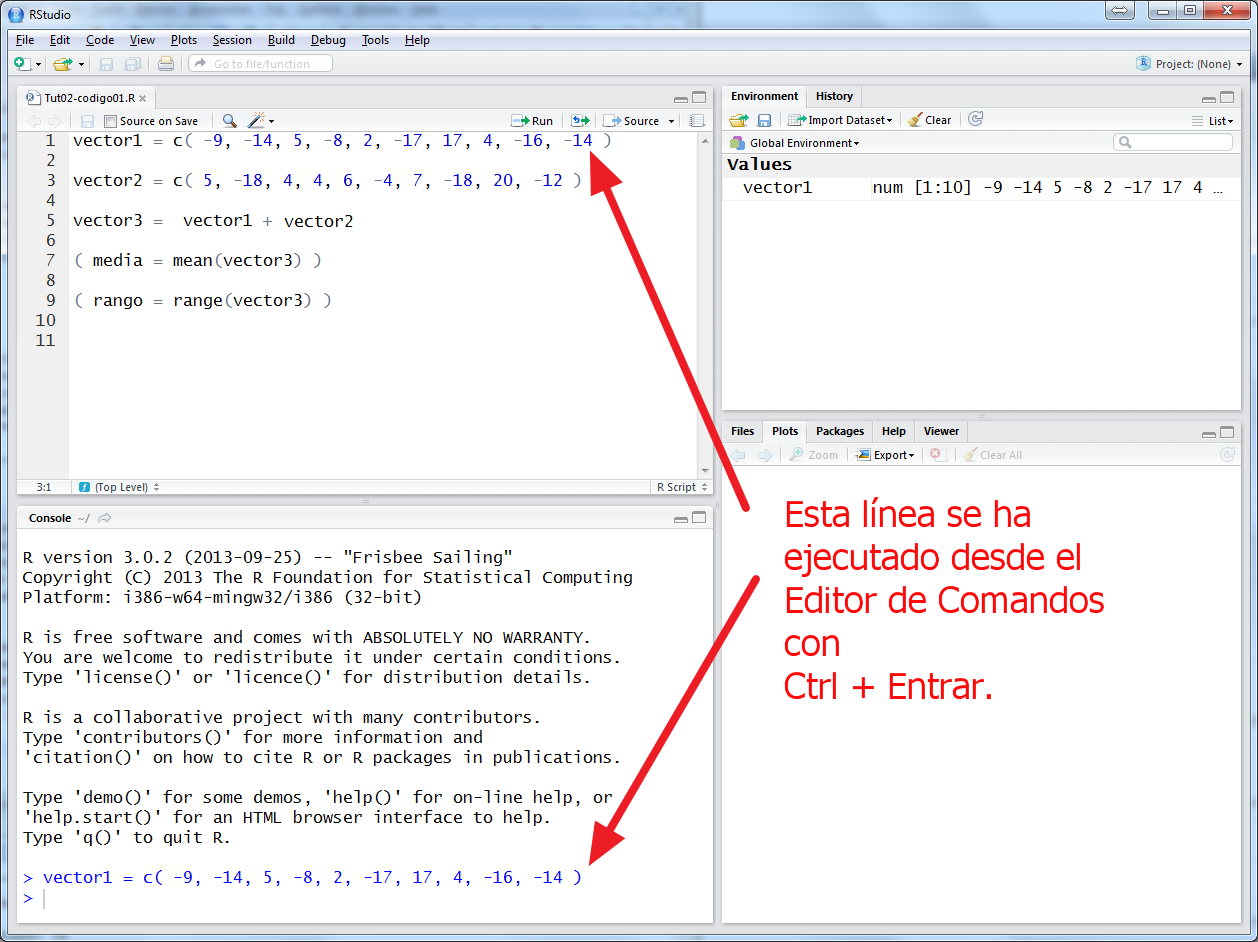
\includegraphics[height=12cm]{../fig/Tut02-20a.png}
    \end{center}
Como indica la figura, la línea de comandos en la que está situado el ratón se transfiere a la {\em Consola de Comandos}, y se ejecuta. Se puede conseguir el mismo resultado si, una vez situado el cursor en la línea deseada, usas el botón {\tt Run}, situado sobre el {\em Editor de Código}:
    \begin{center}
    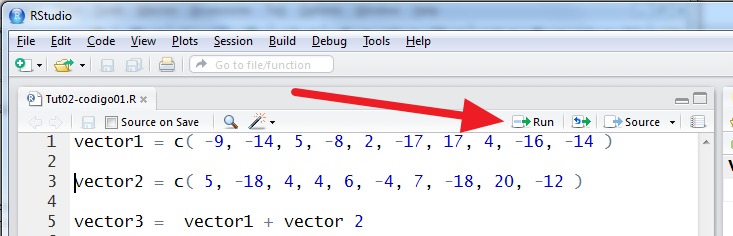
\includegraphics[height=5cm]{../fig/Tut02-21.png}
    \end{center}

\begin{ejercicio}
\label{tut02:ejercicio19}
\quad\\
Prueba a hacer lo mismo con el resto de las líneas de código del fichero, ejecutándolas una por una.
\qed
\end{ejercicio}
Si has hecho este ejercicio, habrás visto que no hay diferencia entre ejecutar un comando desde la {\em Consola} o desde el {\em Editor}, más allá de las teclas que hay que utilizar en cada caso. A cambio, la ejecución desde el {\em Editor} ofrece muchas ventajas. Para empezar, puedes ejecutar todo un grupo de comandos a la vez. Para ver esto, vamos a empezar haciendo limpieza. Pulsa {\tt Ctrl + L} (las dos teclas a la vez), para limpiar la {\em Consola de Comandos}. Ahora, con el ratón o el teclado, selecciona todas las líneas del {\em Editor de Código}. Por cierto, para moverte del {\em Editor de Código} a la {\em Consola de Comandos} y viceversa, puedes usar los atajos de teclado {\tt Ctrl + 1} y {\tt Ctrl + 2}.\\

Asegúrate de que la situación resultado es como la de esta figura (también puedes usar el atajo de teclado {\tt Ctrl + A} para seleccionar todo el código):
    \begin{center}
    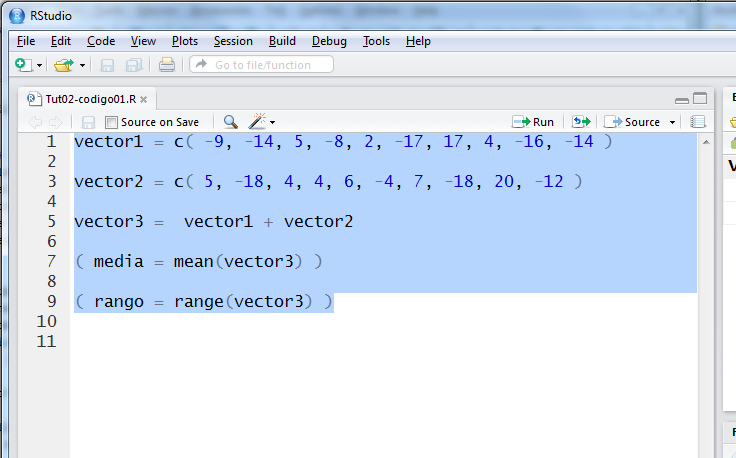
\includegraphics[height=8cm]{../fig/Tut02-22.png}
    \end{center}
Y ahora pulsa {\tt Ctrl + Entrar} (o usa el botón {\tt Run}). Verás que todas esas líneas se ejecutan por orden. Por otra parte, no hace falta que seleccionemos todo el código. Este mecanismo te permite ejecutar parcialmente el código, simplemente seleccionando un bloque de líneas consecutivas, que se ejecutarán desde la primera a la última.
\begin{ejercicio}
\label{tut02:ejercicio20}
\quad\\
Prueba a ejecutar a la vez las líneas $5$ y $7$ del fichero de código (y sólo esas líneas).
\qed
\end{ejercicio}

El {\em Editor de Código} también te permite modificar el fichero de instrucciones sobre el que estamos trabajando. Vamos a  practicar esto.

\begin{ejercicio}
\label{tut02:ejercicio21}
\quad\\
\begin{enumerate}
  \item Cambia las líneas $1$ y $3$ por estas dos:
        \begin{verbatim}
        (vector1 = 1:50 )

        (vector2 = sample(1:50) )
        \end{verbatim}
        No te preocupes por el momento, pronto veremos en detalle como se utiliza la función {\tt sample}. Aquí se limita a ordenar al azar los números del $1$ al $50$.

  \item Añade, en la línea $11$ del {\em Editor de Código}, el comando:
        \begin{verbatim}
        (varMuestral = var(vector3) )
        \end{verbatim}
        y ejecútalo desde el {\em Editor de Código}.

  \item Usa los menús {\tt File}$\to${\tt Save}, o el atajo de teclado {\tt Ctrl + S}, para guardar el fichero modificado. Cierra RStudio, y abre el fichero con un {\em Editor de Texto}. Añade una línea al final del fichero (línea $13$, por ejemplo) con el comando:
        \begin{verbatim}
        boxplot(vector3)
        \end{verbatim}
        Guarda el fichero {\tt Tut02-codigo01.R} modificado, cierra el editor de texto, y vuelve a abrir el fichero en RStudio. Comprueba que aparecen todas las modificaciones que hemos ido haciendo, y ejecuta todos los comandos, al menos un par de veces.
\end{enumerate}
\qed
\end{ejercicio}
Las modificaciones que hemos hecho en este ejercicio no son importantes en sí mismas. El objetivo del ejercicio es demostrar que los ficheros de código de R son simplemente ficheros de texto, que se pueden manipular dentro del propio RStudio, pero también fuera de él, con un editor de texto cualquiera (aunque, como hemos dicho, RStudio ofrece muchas herramientas para hacer nuestro trabajo más cómodo).\\

Eso mismo sucede, en general, con los ficheros de código (a veces decimos {\em código fuente}) de cualquier lenguaje de programación (en inglés, esos ficheros se denominan {\em source code files}). Y, gracias a eso, resulta posible guardar nuestro trabajo muy fácilmente de una vez para otra, o intercambiar esos ficheros con otras personas. Si hemos hecho un análisis estadístico especialmente interesante, y creemos que puede resultar útil para otras personas que estudian problemas parecidos, basta con hacerles llegar nuestro fichero de código, para que puedan repetir ese análisis con sus datos.

Por ejemplo, el fichero adjunto:
\begin{center}
  \fichero{./code/Tut02-codigo02.R}{Tut02-codigo02.R},
\end{center}
contiene (casi todos) los comandos que hemos visto en la Sección \ref{tut03:sec:EstadisticaDescriptivaVariableCuantitativaConR}, para hacer Estadística Descriptiva del vector {\tt var3}. En la Tabla \ref{tut04:tabla:FicheroTut02-codigo02.R} puedes ver el contenido del fichero, que en el caso de ficheros de código llamaremos, a menudo, el {\sf listado del fichero}.

\begin{table}[h!]
\lstinputlisting[numbers=none]{./code/Tut02-codigo02.R}
\caption{Comandos de estadística descriptiva en el fichero {\tt Tut02-codigo02.R}}
\label{tut04:tabla:FicheroTut02-codigo02.R}
\end{table}

Fíjate en que, en la primera fila del fichero, en la línea en la que aparece la función {\tt setwd}, hemos dejado vacío el espacio donde debería estar el nombre del directorio de trabajo (recuerda la discusión de la página \pageref{tut02:lugar:ComandoSetwd}, en la que aprendimos a fijar ese directorio). La razón es fácil de entender: si le enviamos este fichero a otra persona, mi directorio de trabajo no le servirá, y lo primero que tendrá que hacer es cambiar ese directorio de trabajo para que se corresponda con el directorio de su ordenador que vaya a jugar ese papel. Por otra parte, si se desea calcular otros percentiles, hay que modificar el vector de la última línea del código.\\

Evidentemente,  cuando le enviamos el fichero a esa persona, vamos a tener que explicarle estos detalles, si es que queremos que el fichero le sirva de algo. A lo mejor te parece exagerado. Ten en cuenta que este fichero, al ser de los primeros que vemos, es muy sencillo.  Pero a medida que vayamos avanzando en el curso, los ficheros serán cada vez más complejos, y necesitarán cada vez más {``instrucciones de manejo''}. Te podemos asegurar que llegará un momento, no muy lejano, en el que si escribes un fichero de código R, y dejas pasar $15$ días sin usarlo,  cuando lo vuelvas a abrir, pasados esos días, entonces tú mismo, por más que seas el autor del fichero, no recordarás para qué servía aquella variable, o porque hiciste las cosas así y no de otra manera, etc. Una de las verdades más contrastadas por la experiencia sobre la programación es esta:

        \begin{center}
            \fcolorbox{black}{Gris025}{
            \begin{minipage}{7cm}
            {\bf El código sin documentación es inútil.}
            \end{minipage}}
        \end{center}

Ya dijimos, al hablar de Calc en el Tutorial-01, que había que acostumbrarse a identificar las operaciones con una descripción adecuada. En R eso se convierte en una necesidad mucho mayor. Así que, en el próximo apartado, vamos a empezar a aprender a documentar el código en R.


\subsection{Comentarios en R.}
\label{tut02:subsec:ComentariosR}

Documentar significa, en el contexto de los ficheros de código R, añadir a esos ficheros información que no está pensada para dar instrucciones al ordenador, sino que ha sido  pensada para ayudarnos a entender lo que se está haciendo en esa sesión de trabajo. Es decir, esa información no es para la máquina, es para nosotros mismos, o para otros usuarios (humanos) de ese fichero. A lo largo del curso, en los tutoriales, nosotros te vamos a facilitar una serie de ficheros (los llamaremos {\em ``plantillas''}), que contienen código preparado para llevar a cabo algunos de los métodos que vamos a aprender en cada capítulo del curso. Cuando abras por primera vez uno de esos ficheros, y especialmente al tratarse de métodos con los que, aún, no estás familiarizado, necesitarás sin duda unas ``instrucciones de manejo'', para saber como utilizar el fichero. Esas instrucciones podrían ir en un fichero aparte, claro. Pero la experiencia ha demostrado que esa no es una buena manera de organizar el trabajo. Si el código y la documentación van por separado, es casi inevitable que, al final, tras algunos cambios, ya no se correspondan, y la documentación pase a ser contraproducente.  Afortunadamente, hay una manera sencilla de combinar código y documentación. Fíjate en la segunda versión del fichero de comandos de Estadística Descriptiva,
\begin{center}
  \fichero{./code/Tut02-EstadDescriptivaNoAgrup.R}{Tut02-EstadDescriptivaNoAgrup.R}
\end{center}
que aparece en la Tabla \ref{tut02:tabla:Tut02-EstadDescriptivaNoAgrup.R} (pág. \pageref{tut02:tabla:Tut02-EstadDescriptivaNoAgrup.R}). Como puedes ver, hemos añadido al fichero unas líneas nuevas, que empiezan todas con el símbolo \verb&#&. Esas líneas son {\sf comentarios}. Cuando R encuentra el símbolo \verb&#& en cualquier línea de un fichero de código, deja de leer el resto de esa línea. Simplemente lo ignora, y pasa a leer la siguiente línea. Eso nos permite introducir nuestros comentarios, sin que interfieran con el trabajo de R. Si guardas el fichero en el directorio de trabajo y lo abres con RStudio verás que esas líneas aparecen en otro color, para distinguirlas de las líneas normales de código.\\

En el ejemplo de la Tabla \ref{tut02:tabla:Tut02-EstadDescriptivaNoAgrup.R} hemos añadido muchos comentarios, más de uno por cada línea de código. No siempre será necesario ni útil comentar todas y cada una de las líneas; ¡eso puede resultar, a veces, contraproducente! La combinación de unos nombres de variable bien elegidos, y la proporción justa de comentarios es la clave. Pero más vale pecar de exceso de comentarios que lamentar después su falta cuando, al cabo de un tiempo, no seamos capaces de entender el código; ni siquiera nuestro propio código. ¿Cuál es esa proporción justa de comentarios? No hay una respuesta única. Como siempre, \buda{la sabiduría} te llegará (o no...) con el tiempo y la experiencia, cuando hayas visto el trabajo de los demás y desarrolles tu propio estilo. En cualquier caso, como poco deberías incluir unas líneas al principio del fichero explicando para qué sirve ese fichero, quién lo ha escrito, etc.\\

\begin{table}[p]
    \lstinputlisting[numbers=none, firstline=1, lastline=71]{./code/Tut02-EstadDescriptivaNoAgrup.R}
    \caption{Añadiendo comentarios, fichero \fichero{./code/Tut02-EstadDescriptivaNoAgrup.R}{Tut02-EstadDescriptivaNoAgrup.R}. Primera ``plantilla'' de comandos R del curso.}
    \label{tut02:tabla:Tut02-EstadDescriptivaNoAgrup.R}
\end{table}

%\begin{table}[t]
%\lstinputlisting[numbers=none, firstline=49]{./datos/Tut02-EstadDescriptivaNoAgrup.R}
%\caption{Tabla \ref{tut02:tabla:Tut02-EstadDescriptivaNoAgrup.R}, continuación. }
%\end{table}

La segunda ventaja de utilizar comentarios, tal vez no resultará tan evidente al principio de tu trabajo con R. La posibilidad de tratar líneas del fichero como comentarios, y conseguir de esa forma que R las ignore por completo, nos permite {\em ``activar''} o {\em ``desactivar''}, de una forma muy sencilla, partes enteras de un fichero de código R antes de ejecutarlo. Por ejemplo, si cambiamos una línea de código
    \begin{verbatim}
    a=a+1
    \end{verbatim}
por esta otra
    \begin{verbatim}
    # a=a+1
    \end{verbatim}
no estaremos ``explicando'' nada, sino que estamos cambiando el comportamiento de R, y evitando que esa línea en particular se ejecute. Y hacer ese cambio sólo nos cuesta el trabajo de introducir un símbolo \verb&#&. Esto permite tener un único fichero de instrucciones R, que se puede comportar de distinta manera, jugando con los símbolos de comentario. Veremos ejemplos de esto más adelante, y comprobaremos lo práctico que puede llegar a ser.

Cuando hacemos esto, es decir cuando añadimos \verb&#& al comienzo de una línea de código R, decimos que hemos {\em comentado} esa línea (y la {\em descomentamos} cuando quitamos el \verb&#&). Esta operación es bastante frecuente, así que RStudio te ofrece una herramienta, llamada {\tt Comment/Uncomment lines} en el menú {\tt Code}. Si seleccionas una o varias líneas de código, y usas esta opción, verás que RStudio añade \verb&#& al comienzo de todas las líneas comentadas.

    \begin{center}
    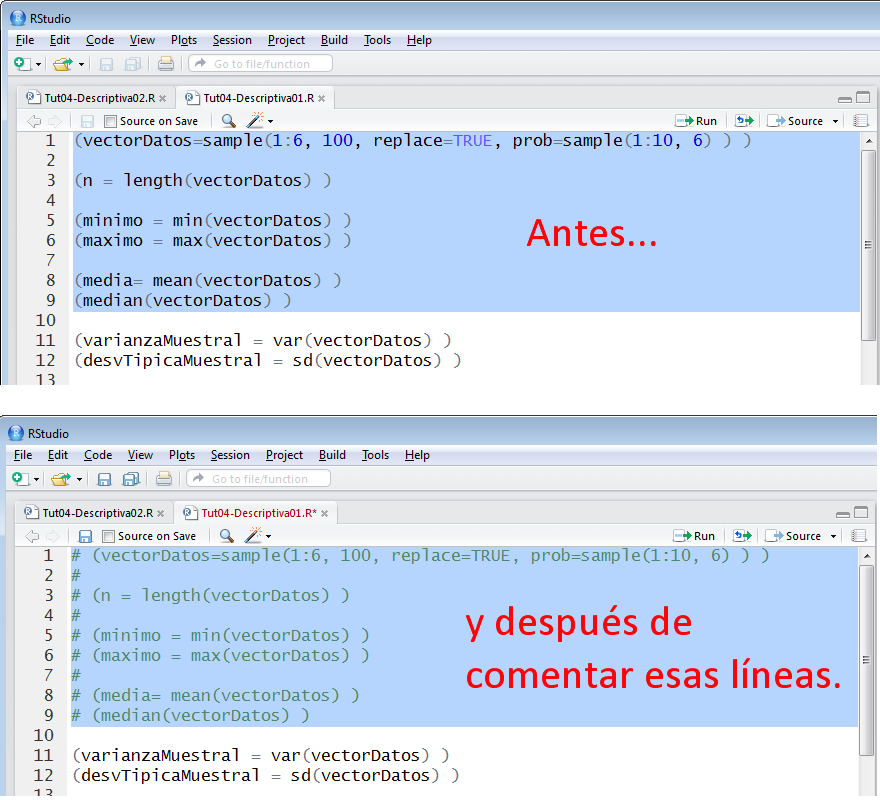
\includegraphics[width=13cm]{../fig/Tut04-07.png}
    \end{center}

No podemos exagerar la importancia de que te acostumbres, desde el primer momento, a incorporar la documentación como una parte inseparable de tu trabajo con R. Te lo recordaremos a menudo, especialmente en los primeros tutoriales. Aparte de esto, la idea de combinar código y documentación se puede llevar, en R, mucho más lejos de lo que aquí hemos visto. Aunque no vamos a poder ocuparnos de ellas en este curso, mediante herramientas como {\em R Markdown}, {\em Sweave} o {\em Knitr}, entre otras, es posible obtener documentos en los que el código R se combina con una documentación mucho más rica, que en algunos casos puede incluir figuras, fórmulas matemáticas complejas, etc.
%Estas técnicas están en la base del movimiento de {\em investigación reproducible} (en inglés {\em Reproducible Research}, sobre el que puedes leer algo más en este enlace de la Wikipedia






\section{Más operaciones con vectores en R.}

Los vectores son un ingrediente esencial de nuestro trabajo con R. En esta sección vamos a (empezar a) aprender cómo fabricar vectores a la medida de nuestros deseos, y a manipular esos vectores con precisión.


\subsection{Números aleatorios: la función sample de R.}
\label{tut02:subsec:NumerosAleatoriosRSample}

En el Tutorial-01 vimos como generar números (pseudo)aleatorios con Calc. Y en el Capítulo \ref{curso-cap:Probabilidad} de la teoría del curso se usan esos números para hacer varios experimentos relacionados con las probabilidades, en situaciones bastante elementales. Para prepararnos, vamos a aprender a hacer lo mismo con R. Como veremos, en este y en futuros tutoriales, se hará evidente que R es un especialista en la materia y, usándolo, vamos a poder ir mucho más allá de lo que resulta viable hacer con Calc.

El primer paso, para empezar a generar números aleatorios con R es utilizar la función {\tt sample}. En su uso más elemental, esta función toma un vector de datos (el que nosotros queramos) y permite elegir al azar $k$ elementos del vector, con o sin reemplazamiento. Y no se agotan ahí sus capacidades, así que vamos a ir viendo diversos ejemplos.

Empezamos por lo más simple, lanzar un dado. Para eso ejecutamos este código:
\begin{verbatim}
    (dado=sample(1:6, size=1) )
\end{verbatim}


Algunas cosas ya nos resultan conocidas. Vamos a guardar el resultado en una variable que hemos llamado {\tt dado}, y hemos rodeado el comando con paréntesis para que R, además de hacer las operaciones que pedimos, nos muestre el resultado. Prueba a ejecutar este comando varias veces seguidas, para ver como, en cada lanzamiento, obtienes un resultado distinto. Naturalmente, esto no sirve si lo que quieres es lanzar el dado muchas veces, pongamos mil veces. Puedes pensar que bastaría con escribir
\begin{verbatim}
    (dado = sample(1:6, size=1000) )
\end{verbatim}
Prueba a ejecutar este comando, y verás que R te obsequia con un bonito mensaje de error:
    \begin{center}
    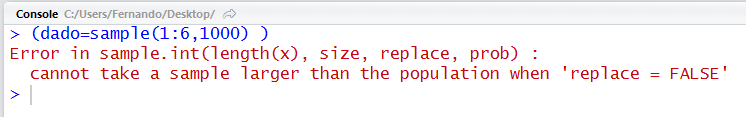
\includegraphics[width=10cm]{../fig/Tut04-01.png}
    \end{center}
El mensaje nos explica cual ha sido el error: hemos tratado de extraer 1000 elementos de un vector que sólo tiene seis, y eso no es posible si {\tt replace=FALSE}, es decir, si el muestreo es sin reemplazamiento. El remedio está claro, hacemos (recuerda que puedes usar el tabulador para ayudarte):
\begin{verbatim}
    (dado = sample(1:6, size=1000, replace = TRUE) )
\end{verbatim}
y, ahora sí, verás desfilar 1000 lanzamientos del dado por tu pantalla. Fíjate en que la variable {\tt dado}, que es el resultado de {\tt sample}, es un vector.
\begin{ejercicio}
\label{tut02:ejercicio22}
\quad\\
\begin{enumerate}
  \item Obtén la tabla de frecuencias, y calcula la media aritmética y la cuasidesviación típica (muestral) de los valores que hay en el vector {\tt dado}.

  \item ¿Cómo puedes comprobar que la variable {\tt dado} es un vector?
\end{enumerate}
Solución en la página \pageref{tut02:ejercicio22:sol}. \qed
\end{ejercicio}

¿Y si en lugar de lanzar un dado mil veces queremos sacar cinco cartas (sin reemplazamiento) de una baraja de 48 cartas? Podemos representar las cartas de la baraja con los números del $1$ al $48$,y entonces basta con hacer:
\begin{verbatim}
(carta = sample(1:48, size=5, replace=FALSE) )
\end{verbatim}

Hasta ahora, hemos visto ejemplos en los que extraíamos valores aleatorios de rangos (o intervalos), como {\tt 1:6}, y {\tt 1:48}. Naturalmente, los rangos no tienen porque empezar en $1$, podemos aplicar {\tt sample} a un rango como {\tt 161:234}. Otras veces, en cambio, nos sucederá que tenemos un vector, como este vector {\tt edades}:
\begin{center}
{\tt
edades = c(22, 21, 18, 19, 17, 21, 18, 20, 17, 18, 17, 22, 20, 19, 18, 19, 18, 22, 20, 19)
}
\end{center}
y lo que queremos es extraer algunos  de estos valores al azar; pongamos por ejemplo, que queremos extraer $7$ elementos. Para hacer eso, si queremos muestreo sin reemplazamiento basta con usar:
\begin{verbatim}
    (edadesAlAzar = sample(edades, size=7, replace=FALSE) )
\end{verbatim}
y si lo queremos con reemplazamiento pondremos {\tt replace=TRUE}. Fíjate en que, en este caso, el vector original ya contiene elementos repetidos. Así que, independientemente de que el muestreo sea con reemplazamiento o sin él, al usar sample podemos obtener valores repetidos. Lo que sample sortea son las {\em posiciones} dentro del vector {\tt edades}, y no los {\em valores} que ocupan esas posiciones.  Para entender esto un poco mejor, prueba a ejecutar este código, en el que usamos {\tt sample} sobre un vector que tiene el número $1$ repetido $9$ veces y un único $2$:
\begin{verbatim}
        muchosUnos = c(1,1,1,1,1,1,1,1,1,2)
        (muestra = sample(muchosUnos, size=100, replace=TRUE) )
\end{verbatim}

Antes de pasar a otras cosas, un truco adicional con la función {\tt sample}. Si aplicas {\tt sample} a un vector, sin ningún argumento más, obtendrás todos los elementos del vector, pero en un orden aleatorio (en lenguaje más técnico, una permutación aleatoria de los elementos del vector). En seguida vamos a ver la función {\tt sort}, que es, en algún sentido, lo contrario de {\tt sample}. La función {\tt sort} ordena, y {\tt sample} desordena. Prueba, por ejemplo a ejecutar varias veces:
\begin{verbatim}
         sample(1:20)
\end{verbatim}
para ver el resultado.


\subsubsection*{Funciones {\tt unique} y {\tt sort}}

A la vista de los últimos ejemplos, y ahora que estamos aprendiendo a fabricar un vector con muchos elementos repetidos, es conveniente subrayar que a veces necesitaremos saber cuáles son los elementos {\em distintos} que contiene ese vector. El recorrido (rango) del vector nos dice el máximo y el mínimo, pero desde luego no nos dice cuáles de los valores intermedios aparecen, de hecho, en el vector. Una manera de obtener esto es mediante la tabla de frecuencias, pero en ese caso el resultado es una tabla, no un vector, y a veces es más difícil de manipular. Afortunadamente, en R tenemos soluciones para todo, y es muy sencillo obtener la respuesta con la función {\tt unique}. Por ejemplo, para el vector {\tt edades} que hemos usado antes, es:
        \begin{verbatim}
        > (edadesDistintas=unique(edades))
        [1] 22 21 18 19 17 20
        \end{verbatim}
Como ves, R devuelve un vector con los valores distintos que hay en {\tt edades}, pero en el orden en que los va encontrando, y no hace ningún esfuerzo por ordenarlos (puede que nos interese conservar el orden, así que eso esta bien).

``¡Pero es que yo los quiero ordenados!'' ¿Hemos dicho ya que en R hay soluciones para todo? Usamos la función {\tt sort}:
    \begin{verbatim}
    > (edadesDistintasEnOrden=sort(unique(edades)))
    [1] 17 18 19 20 21 22
    \end{verbatim}
``Es que las quiero ordenadas en orden decreciente...''
    \begin{verbatim}
    > (edadesDistintasEnOrden=sort(unique(edades), decreasing = TRUE ))
    [1] 22 21 20 19 18 17
    \end{verbatim}
Una aclaración importante sobre {\tt sort}. La ordenación no afecta en absoluto al vector original. Si quieres ordenar un vector, por ejemplo llamado {\tt datos } y guardar el vector ordenado con el mismo nombre, entonces puedes usar el comando
    \begin{verbatim}
        datos = sort(datos)
    \end{verbatim}
pero es importante entender que este es un viaje sin retorno: el vector {\tt datos} original, sin ordenar, se habrá perdido, y sólo tendremos la versión ordenada. ¡Cuidado con la posible pérdida de información relevante!

La función {\tt sort} sirve, desde luego, para ordenar valores numéricos. Pero también hace ordenación alfabética. Vamos a aprovechar para presentarte  un par de vectores especiales, los vectores {\tt letters} y {\tt LETTERS}, que vienen predefinidos en R:
\begin{verbatim}
    > letters
     [1] "a" "b" "c" "d" "e" "f" "g" "h" "i" "j" "k" "l" "m" "n" "o" "p" "q" "r"
    [19] "s" "t" "u" "v" "w" "x" "y" "z"
    > LETTERS
     [1] "A" "B" "C" "D" "E" "F" "G" "H" "I" "J" "K" "L" "M" "N" "O" "P" "Q" "R"
    [19] "S" "T" "U" "V" "W" "X" "Y" "Z"
\end{verbatim}
Como ves, esos vectores contienen las letras del alfabeto (para el idioma inglés). Así que podemos fabricar un vector de letras al azar (¿un generador de contraseñas?) con este código:
\begin{verbatim}
    > ( Clave = sample(LETTERS, size=15, replace=TRUE) )
     [1] "U" "Z" "T" "H" "I" "J" "E" "X" "J" "Y" "P" "G" "V" "P" "P"
\end{verbatim}
Como ves, es un generador de contraseñas muy rudimentario. No te preocupes, en breve podremos hacer uno tan sofisticado como sea preciso. ¿Cuántas letras {\em distintas} aparecen en esa clave? Con las funciones {\tt unique} y {\tt sort} podemos conseguir la respuesta ordenada alfabéticamente:
\begin{verbatim}
    > sort(unique(Clave))
     [1] "E" "G" "H" "I" "J" "P" "T" "U" "V" "X" "Y" "Z"
\end{verbatim}

\begin{ejercicio}
\label{tut02:ejercicio23}
\quad\\
Modifica el generador de claves para que utilice mayúsculas, minúsculas, y cifras. Indicación: recuerda que {\tt c} es por {\em concatenate}. Solución en la página \pageref{tut02:ejercicio23:sol}.
\qed
\end{ejercicio}


\subsubsection*{Números pseudoaleatorios, pero ``reproducibles'': la función {\tt set.seed}.}

Al principio de esta Sección \ref{tut02:subsec:NumerosAleatoriosRSample} hemos lanzado 1000 veces un dado,  con el comando
\begin{verbatim}
    (dado = sample(1:6, size=1000, replace = TRUE) )
\end{verbatim}
El inconveniente de trabajar con números aleatorios es que los resultados del lector serán diferentes de los nuestros y, de hecho, serán diferentes cada vez que ejecutes la función {\tt sample}. Los números aleatorios se utilizan mucho, por ejemplo, para hacer simulaciones. Y si queremos hacer una de esas simulaciones, y compartirla con otras personas, de manera que puedan {\em verificar} nuestros resultados, entonces necesitamos:
\begin{itemize}
  \item Que los números sean aleatorios, en el sentido de que nosotros no los hemos elegido, sino que son el resultado de un {\em sorteo}.
  \item Pero que los resultados del sorteo queden registrados de alguna manera, para que otros puedan reproducirlos.
\end{itemize}
Afortunadamente (en este caso), como ya dijimos, los números que produce un ordenador no son aleatorios, sino pseudoaleatorios. Y para lo que aquí nos ocupa, eso es una ventaja. Hay una función de R, llamada {\sf set.seed}, que permite decirle a R que queremos hacer exactamente esto: generar números aleatorios reproducibles. Concretamente, para ver funciona como esto, prueba en primer lugar a ejecutar varias veces el comando
\begin{verbatim}
    sample(1:100, size=15, replace=TRUE)
\end{verbatim}
Cada vez obtendrás una lista de números diferente. Prueba ahora a ejecutar estos dos comandos:
\begin{verbatim}
    set.seed(2014)
    sample(1:100, size=15, replace=TRUE)
\end{verbatim}
La respuesta será
\begin{verbatim}
    > set.seed(2014)
    > sample(1:100, size=15, replace=TRUE)
     [1] 29 17 63 31 55  9 92 61 10 16 63  6 61 59 66
\end{verbatim}
Y será la misma en tu ordenador, en el mío, o en el de cualquier otra persona que ejecute R. Como ves, la función {\tt set.seed} utiliza un argumento, al que llamamos la {\sf semilla} (en inglés, {\em seed}), que en este caso yo he fijado, arbitrariamente, en $2014$.  La idea es que si utilizas {\tt set.seed} con la misma semilla que yo, obtendrás los mismos números pseudoaleatorios que yo he obtenido.

Una vez visto lo fundamental, no queremos entretenernos mucho más en esto. Pero no podemos dejar de mencionar que el asunto de cómo se elige la semilla es delicado. Podría parecer que lo mejor, en una simulación, es elegir la propia semilla ``al azar''. El problema es que, de esa manera, en caso de que alguien sospeche que se han manipulado los datos, puede pensar que hemos ido probando varias de estas semillas ``al azar'', hasta obtener unos resultados especialmente buenos de la simulación. Muchos autores recomiendan, como alternativa, fijar una política con respecto a la elección de la semilla, y atenerse a ella en todas las simulaciones. Por ejemplo, puedes usar siempre como semilla el año en que realizas la simulación, como hemos hecho aquí.



\subsection{Vectores a medida con {\tt seq} y {\tt rep}.}
\label{tut02:subsec:VectoresMedidaSeqRep}

Ya sabemos que, en R, podemos crear un vector con los números del 1 al 100, basta con usar {\tt 1:100}. Pero habíamos dejado pendiente el problema de conseguir una forma más flexible de fabricar los vectores. ¿Y si queremos, por ejemplo, empezar en 1 y avanzar de 3 en 3, sin pasar de $100$? Es decir, queremos fabricar los números:
\[1,\, 4,\, 7,\,\ldots,\, 94,\, 97,\, 100.\]
Esto se puede conseguir en R de muy fácilmente, usando la función {\tt seq} (de {\em sequence}, secuencia o sucesión, en el sentido matemático del término). Hacemos:
    \begin{verbatim}
        ( deTresEnTres = seq(from =1, to=100, by=3) )
    \end{verbatim}
y obtenemos como respuesta:
    \begin{verbatim}
        > ( deTresEnTres = seq(from =1, to=100, by=3) )
     [1]   1   4   7  10  13  16  19  22  25  28  31  34  37  40
    [15]  43  46  49  52  55  58  61  64  67  70  73  76  79  82
    [29]  85  88  91  94  97 100
    \end{verbatim}
(Ya sabes que el formato de salida y los números entre corchetes dependen de la anchura de tu pantalla). La función {\tt seq} permite fabricar vectores cuyos elementos se diferencian en una cantidad fija; que puede ser cualquier número, entero, fraccionario, expresado con decimales, etc.\\

Recuerda que los argumentos de las funciones de R se pueden escribir con nombre, como hemos hecho aquí (son {\tt from, to, by}). Pero, si sabes lo que haces, también puedes usar:
    \begin{verbatim}
        ( deTresEnTres = seq(1, 100, 3) )
    \end{verbatim}
En cualquier caso, al principio conviene que seas prudente con esto (y recuerda que el tabulador es tu amigo en RStudio).\\
%
%
%
%Vamos a aprovechar este ejemplo para comentar un detalle importante sobre las funciones de R. Podemos escribir el comando anterior de otra forma, más detallada, y el resultado es el mismo:
%    \begin{verbatim}
%        ( deTresEnTres = seq(from=1, to=100, by=3) )
%    \end{verbatim}
%Lo que hemos hecho es usar los nombres de los argumentos de la función. Lo que quizá te sorprenda un poco más es que estas otras versiones también funcionan igual:
%    \begin{verbatim}
%        ( DeTresEnTres = seq(to=100, from=1, by=3) )
%        ( DeTresEnTres = seq(by=3, to=100, from=1) )
%    \end{verbatim}
%En cambio, si pruebas a quitar los nombres en estas dos últimas versiones, verás que la primera directamente no funciona, y que la segunda sí funciona, pero produce otra lista de números.
%    \begin{verbatim}
%        ( DeTresEnTres = seq(100, 1, 3) )
%        ( DeTresEnTres = seq(3, 100, 1) )
%    \end{verbatim}
%¿Cómo funciona este asunto de los argumentos con nombre? Todos los argumentos de todas las funciones de R tienen un nombre. Y cuando queremos asegurarnos de que R nos entiende, y eliminar posibles ambigüedades, lo mejor es usar esos argumentos. Puedes ver la lista de los argumentos consultanto la ayuda (o de forma rápida, con el tabulador como vimos en el \href{Tutorial-03.pdf}{Tutorial03}). ¿Y qué sucede cuando no usamos los nombres? En ese caso, R interpreta los argumentos que recibe en orden. colocándolos en las posiciones que le parecen correctas. Por ejemplo, para la función {\tt seq}, R espera, en ese orden, que los tres primeros argumentos sean:
%    \begin{verbatim}
%        seq(from=... , to=... , by=... , )
%    \end{verbatim}
%Y si recibe tres números los va a colocar en esas posiciones. Esto nos permite trabajar rápido cuando tenemos prisa... y sabemos lo que hacemos. Si tienes dudas, recuerda que el tabulador es tu amigo.

La función {\tt seq} es, además, muy útil para dividir un intervalo $(a,b)$ en $n$ subintervalos iguales (esto te vendrá bien, por ejemplo, cuando quieres dividir los valores de una variable cuantitativa continua en clases). Podríamos hacer las cuentas ``a mano'', calculando la longitud de los subintervalos, etc. Pero {\tt seq} facilita mucho el trabajo, remplazando la opción {\tt by} con la opción {\tt length.out}, que debes interpretar como {\em cuántos valores quieres que contenga el vector de salida}. Por ejemplo, si quiero dividir el intervalo $(15,27)$ en $19$ subintervalos iguales, teniendo en cuenta que se incluyen los extremos, está claro que necesito $19+1=20$ puntos en el vector de salida. En este tipo de situaciones es típico usar el nombre {\sf nodos} para los extremos de los subintervalos que vamos a fabricar (no los confundas con las marcas de clase, que son los puntos medios de esos subintervalos). Así que hacemos
    \begin{verbatim}
        (nodos = seq(from=15 , to=27 , length.out=20 ) )
    \end{verbatim}
La respuesta es justo lo que queríamos:
\begin{verbatim}
> (nodos = seq(from=15 , to=27 , length.out=20 ) )
 [1] 15.00000 15.63158 16.26316 16.89474 17.52632 18.15789 18.78947 19.42105
 [9] 20.05263 20.68421 21.31579 21.94737 22.57895 23.21053 23.84211 24.47368
[17] 25.10526 25.73684 26.36842 27.00000
\end{verbatim}

Hay otra función, la función {\tt rep} (de {\em repeat}, repetir), estrechamente emparentada con {\tt seq}, cuyo principal uso es fabricar vectores, siguiendo un patrón que nosotros definimos. El nombre {\tt rep} viene de repeat, repetir. Y eso ayuda a adivinar lo que sucede si escribimos este comando:
    \begin{verbatim}
    valores = c(1,2,3,4,5)
    rep(valores, times=3)
    \end{verbatim}
El argumento {\tt times} (en inglés, aquí con significado de  {\em ``veces''}). La salida correspondiente es, como cabría esperar, el vector datos repetido tres veces:
    \begin{verbatim}
    > valores=c(1,2,3,4,5)
    > rep(valores, times=3)
    [1] 1 2 3 4 5 1 2 3 4 5 1 2 3 4 5
    \end{verbatim}
Por cierto, ese argumento opcional {\tt times} es uno de los raros casos que no se obtiene con el tabulador en RStudio.\\

Quizá sea un poco menos fácil adivinar lo que sucede con este otro comando:
    \begin{verbatim}
    valores = c(1, 2, 3, 4, 5)
    rep(valores, times=c(2, 9, 1, 4, 3) )
    \end{verbatim}
Si lo ejecutamos,  la salida es:
    \begin{verbatim}
    > valores = c(1, 2, 3, 4, 5)
    > rep(valores, c(2, 9, 1, 4, 3) )
    [1] 1 1 2 2 2 2 2 2 2 2 2 3 4 4 4 4 5 5 5
    \end{verbatim}
Y ahora está más claro lo que sucede: el segundo argumento le dice a R cuántas veces debe repetir cada uno de los correspondientes elementos del vector datos (el primer argumento). Aquí el vector que usamos en {\tt times} juega el papel de {\em vector de frecuencias} para los elementos del vector {\tt valores}.

Por eso, este funcionamiento de rep es especialmente interesante cuando tenemos que empezar a trabajar a partir de datos representados mediante tablas de frecuencias. Para ver un ejemplo sencillo, vamos a suponer que tenemos dos vectores:
    \begin{verbatim}
    valores = c(2,3,5,8,13)
    frecuencias = c(5,7,12,2,14)
    \end{verbatim}
de manera que el primero contiene los valores (distintos) que aparecen en nuestros datos, y el segundo contiene las frecuencias de esos valores (por supuesto, los dos vectores tendrán la misma longitud). Entonces, para recuperar el conjunto inicial de datos (sin agrupar) partiendo de esta ``tabla de frecuencias'', podemos usar así la función {\tt rep}:
    \begin{verbatim}
    ( datosSinAgrupar = rep(valores, times=frecuencias) )
    \end{verbatim}
Y se obtiene este resultado:
    \begin{verbatim}
    > ( datosSinAgrupar = rep(valores, frecuencias) )
     [1]  2  2  2  2  2  3  3  3  3  3  3  3  5  5  5  5  5  5  5  5  5  5  5  5
    [25]  8  8 13 13 13 13 13 13 13 13 13 13 13 13 13 13
    \end{verbatim}
Ahora puedes utilizar las funciones habituales para hacer la Estadística Descriptiva del vector {\tt datosSinAgrupar}. Esta forma de ``desempaquetar'' tablas de frecuencia nos será útil en ocasiones.

En este último ejemplo hemos usado una ```tabla de frecuencias'' que en realidad no es una tabla, sino dos vectores por separado, uno con los valores y otro con las frecuencias.  Para ver con más claridad, el  fichero csv \fichero{../datos/tut04-EjemploTablaFrecuencias.csv}{tut04-EjemploTablaFrecuencias.csv} contiene esta misma tabla de frecuencias. Pero si pruebas a guardarlo en la subcarpeta {\tt datos}, para leerlo con la función {\tt scan} que vimos en el Tutorial03, no te va a resultar fácil, porque {\tt scan} no está pensada para eso (puedes abrirlo con un editor de texto para examinarlo). En próximos tutoriales veremos como trabajar con este tipo de tablas en R, y entre otras cosas, aprenderemos a leerlas a partir de un fichero csv.



% las ideas max(table), length()-length(unique()) y sort()

\subsection{Seleccionando elementos de vectores.}

\subsubsection*{La notación de corchetes. Funciones {\tt head} y {\tt tail}.}

Volvemos entonces a nuestros $1000$ lanzamientos del dado, pero ahora vamos a hacer:
\begin{verbatim}
    set.seed(2014)
    dado = sample(1:6, size=1000, replace = TRUE)
\end{verbatim}
De esa forma,  el lector y nosotros trabajaremos sobre el mismo vector {\tt dado}, y podrás comparar tus resultados con los nuestros. En el Ejercicio \ref{tut02:ejercicio22} (pág. \pageref{tut02:ejercicio22}) hemos invitado al lector a que hiciera la tabla de frecuencias del vector {\tt dado}, resultante de ese experimento. El resultado de aquel ejercicio (para el vector {\tt dado} que hemos fabricado después de usar {\tt set.seed}) es:
\begin{verbatim}
    > table(dado)
    dado
      1   2   3   4   5   6
    145 154 167 192 167 175
\end{verbatim}
Eso nos permite, por ejemplo, ver que el número 5 ha aparecido $167$ veces. Pero no nos permite saber cuál fue el resultado de la tirada número 23.  Para averiguar esto, en R escribimos
\begin{verbatim}
    > dado[23]
    [1] 4
\end{verbatim}
y vemos que en esa tirada se obtuvo un $4$. De esa forma, usando los corchetes, podemos acceder directamente a cualquier posición del vector. Por ejemplo, el primer y el último elemento del vector son:
\begin{verbatim}
    dado[1]
    dado[length(dado)]
\end{verbatim}
En este caso sabemos que el vector tiene 1000 elementos, y para obtener el último elemento podríamos haber escrito
\begin{verbatim}
    dado[1000]
\end{verbatim}
pero la otra versión (usando length) tiene la ventaja de que seguirá funcionando aunque el vector cambie. Si quieres ver unos cuantos valores del principio (respectivamente del final) del vector, puedes usar {\tt head(dado)} (respectivamente, {\tt tail(dado)}). Estas dos funciones, por defecto, te mostrarán los últimos seis elementos del vector, pero puedes usar el argumento opcional {\tt n} para controlar cuántos se muestran.

\begin{ejercicio}
\label{tut02:ejercicio24}
\quad\\
Usa la función {\tt tail} para obtener el último elemento del vector {\tt dado}. Solución en la página \pageref{tut02:ejercicio24:sol}.
\qed
\end{ejercicio}

Aunque las funciones {\tt head} y {\tt tail} son útiles, la herramienta básica para acceder a los elementos de un vector son los corchetes {\tt [\,]} (en inglés, {\em (square) brackets}). Este recurso de los corchetes es mucho más potente de lo que parece a primera vista. Podemos seleccionar varios elementos a la vez indicando sus posiciones. Para seleccionar los elementos de dado en las posiciones de la 12 a la 27 hacemos:
\begin{verbatim}
    > dado[12:27]
     [1] 1 4 4 4 3 5 1 6 2 6 5 4 5 4 6 3
\end{verbatim}
y obtenemos un vector con los números que ocupan exactamente esas posiciones. Y si las posiciones que queremos no son consecutivas, basta con indicarlas mediante un vector (no olvides la {\tt c} al crear el vector). Por ejemplo:
\begin{verbatim}
    > dado[c(3,8,21,43,56)]
    [1] 4 4 6 6 1
\end{verbatim}
nos proporciona los elementos en esas posiciones del vector. Cuando se combina esto con otras ideas, que estamos viendo en este tutorial, se pueden conseguir resultados muy útiles. Por ejemplo, ¿qué crees que sucede al hacer esto? (Haz el experimento).
\begin{verbatim}
    datos=100:200
    datos
    datos[seq(1,length(datos),3)]
\end{verbatim}

\subsubsection*{Selección de elementos mediante condiciones. Valores booleanos. Función {\tt which}.}
\label{tut02:subsubsec:SeleccionElementosCondicionesValoresBooleanosWhich}

Pero aún podemos ir más lejos. Podemos utilizarlo para seleccionar los elementos del vector que cumplen cierta condición. Por ejemplo, queremos seleccionar los resultados, en el vector {\tt dado}, que son mayores que 3. En primer lugar, igual que aprendimos (en el anterior tutorial) a sumar una cantidad a un vector, o a elevar un vector al cuadrado, etc., podemos también aplicar una condición lógica, como una desigualdad, a un vector (¡no ejecutes el comando todavía!):
\begin{verbatim}
    dado > 3
\end{verbatim}
Tienes que aprender a leer esta expresión como si fuera una pregunta: ``¿Es el resultado de lanzar el dado mayor que $3$?''. La respuesta sólo puede ser ``sí'' o ``no'', o dicho de otra manera ``cierto'' o ``falso'' \footnote{en realidad hay un tercer caso, del que ya hablaremos, cuando el elemento del vector está ausente, como los valor {\tt NaN} que ya hemos visto.}. En R (y en muchos lenguajes de programación), las respuestas a ese tipo de preguntas se representan con un tipo especial de variables, las {\sf variables  booleanas} (por el matemático G. Boole\footnote{Más información en  \link{http://es.wikipedia.org/wiki/George\_Boole}{http://es.wikipedia.org/wiki/George\_Boole}}). Una variable de tipo booleano, por tanto, sólo puede tomar dos valores, que son {\tt TRUE} (cierto) o {\tt FALSE} (falso). Las variables de tipo booleano son esenciales en programación. Un programa tiene que tomar muchas decisiones del estilo ``si la condición C es cierta, haz la acción A, y si no, haz la acción B''. Esas decisiones dependen del resultado de la ``condición C'', que siempre es una variable booleana. Veremos ejemplos, usando R, en futuros tutoriales.


¿Cuál es el resultado de {\tt dado < 3}? Pues un vector de $1000$ valores booleanos. Para ver los $10$ primeros vamos a hacer:
\begin{verbatim}
    > head( dado < 3, n=10)
     [1]  TRUE  TRUE FALSE  TRUE FALSE  TRUE FALSE FALSE  TRUE  TRUE
\end{verbatim}
Y para que puedas comprobar de donde proceden esos valores,  aquí tienes los $10$ primeros elementos de {\tt dado}.
\begin{verbatim}
    > head( dado , n=10)
     [1] 2 2 4 2 4 1 6 4 1 1
\end{verbatim}
Cada elemento del vector booleano que se obtiene con {\tt dado < 3} nos dice si la condición ``es mayor que 3'' es cierta o falsa en la correspondiente posición de {\tt dado}.


Las cosas empiezan a ponerse divertidas cuando combinamos esta idea con la selección por corchetes, por ejemplo, así:
\begin{verbatim}
    mayoresQue3 = dado[ dado > 3 ]
\end{verbatim}
Entonces, en el vector {\tt mayoresQue3} obtenemos un vector que contiene precisamente aquellos elementos de {\tt dado} que eran mayores que 3 (por lo tanto, que valen $4$, $5$ o $6$):
\begin{verbatim}
    > mayoresQue3
      [1] 4 4 6 4 4 4 4 4 5 6 6 5 4 5 4 6 6 5 6 5 4 5 5 5 4 6 6 4 5 4 5 6 5 6 4
     [36] 4 6 5 4 6 5 5 4 4 5 5 5 5 6 6 4 6 4 4 5 4 5 6 4 6 5 5 5 6 4 4 4 4 4 6
     [71] 6 4 6 4 4 6 6 6 5 4 4 6 4 5 5 4 6 4 4 4 6 4 5 6 4 6 6 5 5 5 5 5 4 5 6
    [106] 5 4 6 5 5 5 6 4 6 4 6 6 4 4 4 5 4 5 6 4 4 5 6 6 5 4 5 6 5 4 5 4 6 4 5
    [141] 5 6 6 4 4 6 4 4 4 6 5 5 6 4 6 4 4 6 5 6 4 4 6 6 5 6 5 5 6 6 4 4 6 4 5
    [176] 6 4 5 6 6 4 6 4 5 4 5 4 6 4 5 5 4 5 5 4 6 6 6 5 6 4 4 4 4 4 4 5 5 6 6
    [211] 6 4 6 6 6 4 5 6 4 5 5 4 6 6 4 5 5 4 4 4 4 4 6 6 4 5 5 6 5 6 4 6 6 6 4
    [246] 6 6 5 5 5 6 6 5 5 4 4 5 4 4 6 6 6 5 6 4 6 6 6 4 6 6 5 4 5 5 6 6 6 5 4
    [281] 5 4 4 6 5 5 6 4 4 5 5 6 4 4 5 6 6 6 6 4 6 5 4 4 6 6 5 6 6 4 4 6 6 6 4
    [316] 6 5 4 6 5 5 4 6 5 5 6 6 4 6 4 6 5 6 5 4 5 4 4 6 6 6 6 4 4 4 5 4 6 6 6
    [351] 6 5 4 6 6 6 6 5 6 6 5 6 4 6 4 5 4 5 6 5 6 5 6 5 4 5 5 5 5 6 4 4 5 6 5
    [386] 5 5 4 4 5 4 4 6 4 6 4 5 5 4 5 5 5 4 6 5 4 4 6 6 6 4 5 5 5 6 5 4 6 4 4
    [421] 5 6 5 6 6 5 5 5 4 6 6 4 4 4 6 4 5 5 6 4 4 4 5 4 5 6 4 5 5 5 4 5 5 5 6
    [456] 5 6 6 5 4 6 6 4 6 5 5 5 6 6 5 4 4 4 5 4 5 5 6 5 4 6 4 4 6 5 5 5 4 4 6
    [491] 4 4 5 5 4 4 4 6 4 4 4 6 4 4 5 4 4 4 6 4 5 6 5 6 5 4 4 5 5 5 5 5 4 4 4
    [526] 6 4 4 5 4 6 4 5 4
\end{verbatim}

Pero claro, en este vector hemos perdido la información sobre las posiciones originales que ocupaban esos valores en {\tt dado}. Si quieres obtener esa información, usa la función {\tt which} junto con la condición {\tt dado > 3}:
\begin{verbatim}
which( dado > 3 )
\end{verbatim}
Y obtendrás un vector de posiciones (sólo se muestra el principio, usando {\tt head}):
\begin{verbatim}
> head( which( dado > 3 ), n=20)
 [1]  3  5  7  8 11 13 14 15 17 19 21 22 23 24 25 26 30 31 35 36
\end{verbatim}
Para que quede claro: si miras el vector {\tt dado}, en una de estas posiciones, encontrarás un valor mayor que $3$. Y viceversa si la posición no aparece en esta lista, entonces el correspondiente valor de {\tt dado}, será $3$ o menos.
\begin{ejercicio}
\label{tut02:ejercicio25}
\quad\\
\begin{enumerate}
  \item Comprueba que en la posición número $16$ de {\tt dado} (que no aparece arriba), hay un elemento menor o igual que $3$.
  \item Construye un vector que contenga las posiciones de {\tt dado} que contienen números mayores o iguales que $2$.
  \item Un poco más difícil. Construye un vector que contenga las posiciones de {\tt dado} que contienen números pares. Pista: ¿qué hacía el operador \verb#%%# (ver el Ejercicio \ref{tut02:ejercicio01}, pág. \pageref{tut02:ejercicio01})?
\end{enumerate}
Solución en la página \pageref{tut02:ejercicio25:sol}.\qed
\end{ejercicio}

Como puedes ver, nuestra capacidad de fabricar vectores a medida, muestrearlos (samplearlos) y seleccionar sus elementos, es muy grande. ¡Y ni siquiera hemos hablado aún de la función {\tt paste}, que es probablemente una de las herramientas más versátiles para generar vectores en R! Esta función es extremadamente útil en Diseño Experimental, y hablaremos de ella en alguno de los próximos tutoriales.

\subsubsection*{Los valores booleanos como unos y ceros. Operadores booleanos.}
\label{tut02:subsubsec:BooleanosComoUnosCeros}

Ya hemos dicho que los valores booleanos {\tt TRUE} y {\tt FALSE} son la base sobre la que se construye toda la toma de decisiones, en R y, en general, en cualquier programa de ordenador. Las decisiones se toman comprobando si se cumple una cierta condición, que, a veces, puede ser tan sencilla como las que hemos visto:
\begin{verbatim}
     dado > 3
\end{verbatim}
En cuanto esa condición sea un poco más complicada, necesitaremos más herramientas. Por ejemplo, si queremos seleccionar los elementos del vector {\tt dado} que son, \underline{\em a la vez}, más grandes que $3$ y menores que $6$, entonces necesitamos aprender una forma de expresar la conjunción ``Y'' en el lenguaje de R. En ese lenguaje, esto se expresa así:
\begin{verbatim}
     (dado > 3) & (dado < 6)
\end{verbatim}
El operador {\tt \&} es, en R, el {\sf Y booleano} (en inglés se escribe a menudo {\em AND}, en mayúsculas). En otros lenguajes de programación se escribe de diferentes maneras. Para ver como funciona el operador {\tt \&}, vamos a ejecutar varios comandos:
\begin{verbatim}
    > TRUE & TRUE
    [1] TRUE
    > TRUE & FALSE
    [1] FALSE
    > FALSE & TRUE
    [1] FALSE
    > FALSE & FALSE
    [1] FALSE
\end{verbatim}
Estos cuatro comandos cubren todas las situaciones posibles al usar {\tt \&}. Por ejemplo, al evaluar una condición como:
\begin{verbatim}
  (3 < 5) & (6 < 4)
\end{verbatim}
el primer paréntesis da como resultado {\tt TRUE} y el segundo {\tt FALSE}, así que (estamos en el segundo caso y) el operador {\tt \&} produce {\tt FALSE}:
\begin{verbatim}
    > (3 < 5) & (6 < 4)
    [1] FALSE
\end{verbatim}
Como ves, para que el resultado de {\tt \&} sea {\tt TRUE} es necesario que ambos operandos sean {\tt TRUE}.
Otro operador booleano de R, estrechamente emparentado con {\tt \&}, es el operador {\tt |} (una barra vertical), llamado {\sf O booleano} (en inglés se escribe a menudo {\em OR}. Todo lo que se necesita saber de este operador se resume en estas cuatro situaciones posibles:
\begin{verbatim}
> TRUE | TRUE
[1] TRUE
> TRUE | FALSE
[1] TRUE
> FALSE | TRUE
[1] TRUE
> FALSE | FALSE
[1] FALSE
\end{verbatim}
con la que no deberías tener problemas en hacer el siguiente:
\begin{ejercicio}
\label{tut02:ejercicio26}
\quad\\
¿Cuál es el resultado de la siguiente operación?
\begin{verbatim}
    (7 < 5) | (2 < 4)
\end{verbatim}
Solución en la página \pageref{tut02:ejercicio26:sol}.\qed
\end{ejercicio}
Como ves, el comportamiento de {\tt |} es simétrico al de {\tt \&}. Para que el resultado de {\tt |} sea {\tt FALSE} es necesario que ambos operandos sean {\tt FALSE}.

R utiliza un sistema de equivalencia entre los valores booleanos {\tt TRUE} y {\tt FALSE} por un lado, y los números {\tt 1} y {\tt 0} por otro, que resulta a menudo extremadamente útil. Si le pedimos a R que {\em multiplique} {\tt TRUE} por {\tt FALSE}, lo que hará será cambiar {\tt TRUE} por $1$, {\tt FALSE} por $0$, multiplicar, obteniendo un $0$:
\begin{verbatim}
> TRUE * FALSE
[1] 0
\end{verbatim}
Puedes hacer lo mismo para hacer cualquier operación con los valores lógicos. Por ejemplo,
\begin{verbatim}
    > TRUE/FALSE
    [1] Inf
    > TRUE + TRUE
    [1] 2
    > TRUE + FALSE
    [1] 1
\end{verbatim}
Los dos últimos resultados permiten usar los valores booleanos para {\em contar} los elementos de un vector que verifican una condición. En efecto, hemos visto que con la condición
\begin{verbatim}
     dado > 3
\end{verbatim}
se obtiene como respuesta un vector booleano de valores {\tt TRUE} y {\tt FALSE} que nos dicen, para cada elemento del vector {\tt dado}, si esa condición es cierta o no. Para saber cuántos elementos la cumplen, es decir, cuántos valores {\tt TRUE} hay en el vector booleano {\tt dado > 3}, basta con tener en cuenta que los valores {\tt TRUE} cuentan como $1$ y los {\tt FALSE} como $0$, y {\em sumar} ese vector booleano:
\begin{verbatim}
    > sum(dado >3)
    [1] 534
\end{verbatim}
Si tienes problemas para entender esto, piensa que el resultado de {\tt dado > 3} es un vector de unos y ceros, y que lo que queremos es saber cuántos unos contiene.

Hemos visto que R convierte {\tt TRUE} en $1$ y {\tt FALSE} en $0$. Es bueno saber que R también hace conversiones en sentido contrario. Si usas los operadores lógicos {\tt \&} y {\tt |} para operar {\em con números}, entonces el número $0$ se convierte en {\tt FALSE}, mientras que {\em cualquier otro número} se convierte en {\tt TRUE}. Por ejemplo:
\begin{verbatim}
    > 3 & 5
    [1] TRUE
    > 3 & 0
    [1] FALSE
    > 0 | 2
    [1] TRUE
    > 0 | 0
    [1] FALSE
    > -2.3 & 0
    [1] FALSE
\end{verbatim}
El último ejemplo pretende ilustrar que las mismas reglas funcionan con números fraccionarios o negativos. Recuerda: cualquier cosa que no sea un $0$ se convierte en {\tt TRUE}.


\subsubsection*{El operador ``igual a''}

Hemos visto cómo seleccionar los elementos del vector {\tt dado} que son mayores que $3$. Pero ¿y si necesitamos seleccionar aquellos que son exactamente iguales a $3$? Tu primera reacción tal vez sea escribir
\begin{verbatim}
  dado[dado=3]
\end{verbatim}
pero eso no funcionará como esperas, porque en R, el símbolo {\tt =} indica, como ya sabemos, una {\em asignación} de una variable a un valor. El significado de {\tt =} es más bien {\tt usa esta etiqueta para este valor}. Y lo que ahora necesitamos es una forma de decidir si dos valores son iguales. El operador adecuado, en R, se representa con dos símbolos igual concatenados:
\begin{verbatim}
    > 3 == 5
    [1] FALSE
    > 3 == 3
    [1] TRUE
\end{verbatim}
y, al igual que sucede con {\tt >}, o con {\tt <}, es un operador booleano, que produce como resultado {\tt TRUE} o {\tt FALSE} (o {\tt NA} si alguno de los argumentos es igual a {\tt NA}).

Volviendo a la pregunta inicial, la forma de localizar los elementos de {\tt dado} que son iguales a $3$ es
\begin{verbatim}
    dado[dado == 3]
\end{verbatim}


\begin{ejercicio}
\label{tut02:ejercicio27}
\quad\\
Ejecuta estas instrucciones:
\begin{verbatim}
    set.seed(2014)
    dado2 = sample(1:6, 1500, replace = TRUE)
\end{verbatim}
¿Cuántos elementos del vector {\tt dado2} son iguales a $4$? Responde sin usar {\tt table}. Solución en la página \pageref{tut02:ejercicio27:sol}.
\qed
\end{ejercicio}


\section{Formato del código R en próximos tutoriales.}
\label{tut02:sec:FormatoCodigoR}

En este tutorial hemos tratado de presentar el código en R de la forma que creemos resulta más natural para los usuarios que acaban de iniciarse en el manejo del sistema. Esa presentación tiene, como decimos, la ventaja de la naturalidad, pero no es la más cómoda para el trabajo que vamos a hacer en el resto del curso. En los próximos tutoriales vamos a utilizar un sistema diferente, pensado para hacer tu trabajo más cómodo. No te lo hemos presentado del principio porque creemos que, sin conocer un poco el funcionamiento de R, podría crear confusión.

¿De qué se trata? Vamos a usar como ejemplo una simulación del lanzamiento de un dado $1000$ veces, en la que calcularemos además la media, el rango intercuartílico y la cuasidesviación típica del vector de resultados. Hasta ahora, para mostrarte el código necesario, y los resultados que produce, hemos usado un formato como este.
\begin{verbatim}
> set.seed(2014)
> dado = sample(1:6, 1000, replace=TRUE)
> mean(dado)
[1] 3.607
> IQR(dado)
[1] 3
> sd(dado)
[1] 1.674322
\end{verbatim}
Ese formato está bien, en tanto que reproduce de una forma fiel el ``diálogo'' que mantenemos con R. Pero si quieres copiar ese código desde este documento, para pegarlo en RStudio, por ejemplo, y así poder ejecutarlo o modificarlo a tu gusto, entonces aparecen algunos inconvenientes. Para empezar, al copiar las líneas de comandos estarás copiando también el símbolo {\tt >} (el {\em prompt} de R). Y eso significa que tienes que eliminar ese símbolo antes de ejecutar la línea de código. Además, estarás copiando también las líneas de resultados, que no puedes ejecutar sin que se produzcan errores. En resumen, no es un formato cómodo, y lo va a ser cada vez menos a medida que avancemos en el curso. Para evitar esos problemas, vamos a utilizar este otro formato:
\begin{knitrout}
\definecolor{shadecolor}{rgb}{0.969, 0.969, 0.969}\color{fgcolor}\begin{kframe}
\begin{alltt}
\hlkwd{set.seed}\hlstd{(}\hlnum{2014}\hlstd{)}
\hlstd{dado} \hlkwb{=} \hlkwd{sample}\hlstd{(}\hlnum{1}\hlopt{:}\hlnum{6}\hlstd{,} \hlnum{1000}\hlstd{,} \hlkwc{replace}\hlstd{=}\hlnum{TRUE}\hlstd{)}
\hlkwd{mean}\hlstd{(dado)}
\end{alltt}
\begin{verbatim}
## [1] 3.607
\end{verbatim}
\begin{alltt}
\hlkwd{IQR}\hlstd{(dado)}
\end{alltt}
\begin{verbatim}
## [1] 3
\end{verbatim}
\begin{alltt}
\hlkwd{sd}\hlstd{(dado)}
\end{alltt}
\begin{verbatim}
## [1] 1.674322
\end{verbatim}
\end{kframe}
\end{knitrout}
Como ves, aparte de los colores y el sombreado (que no son importantes), en este formato ha desaparecido el {\em prompt} {\tt >} de R. Así que puedes copiar las líneas de código completas en RStudio y ejecutarlas directamente sin problemas.Además, para facilitar la copia de bloques enteros de líneas de código, las líneas con respuestas de R (líneas de salida) se muestran comentadas (precedidas por \verb/#/). De esa manera, aunque las copies a RStudio no causarán ningún efecto sobre la ejecución de los comandos. Este formato para el código y las respuestas simplificará mucho  nuestro trabajo en el resto del curso. Y más adelante, en un tutorial opcional explicaremos en detalle la herramienta que hemos usado, porque su utilidad va mucho más allá de un simple cambio de formato.


\section{Ejercicios adicionales y soluciones.}
\label{tut02:sec:SolucionesEjerciciosAdicionales}

\subsection*{Ejercicios adicionales.}


\begin{enumerate}
  \addtocounter{enumi}{27}
  \item En todos los ejemplos de aritmética vectorial que hemos visto, los dos vectores implicados eran de la misma longitud. ¿Qué sucede si no es así? Pues algo interesante, y que en cualquier caso conviene conocer para evitar errores. Te invitamos a que lo descubras ejecutando este ejemplo:
    \begin{center}
    \begin{minipage}{12cm}
    {\tt
    vector3=c(1,2,3,4,5,6,7,8,9,10,11,12,13,14,15,16,17,18,19,20)\\
    vector4=c(0,1,2)\\
    vector3+vector4
    }
    \end{minipage}
    \end{center}
    ¿Qué ha hecho R? Puedes entenderlo así: al principio empieza sumando normalmente, posición a posición. Pero tras sumar tres posiciones, R descubre que {\tt vector4} se ha agotado. Y lo que hace es simplemente volver al principio de {\tt vector4} y comenzar de nuevo a utilizar sus elementos desde el primero. Así pues, en el resultado,  se suma el vector 0,1,2 con 1,2,3 y luego se vuelve a sumar 0,1,2 con 4,5,6, (para dar 4,6,8 de resultado) y así, consecutivamente, vamos recorriendo la suma hasta que el vector más largo, {\tt vector3}, se agota a su vez.

    Como ejercicio para practicar esto: dado el vector {\tt vector1 = 68:213}, súmale un {\tt vector2}, de longitud $5$, de manera que todos los elementos de {\tt vector1 + vector2} sean múltiplos de $5$.

  \item En el Tutorial-01 hemos visto cómo calcular la media, varianza, etc. a partir de una tabla de frecuencias de una variable cuantitativa discreta (recuerda, para empezar, la Sección \ref{tut01-tut02:sec:mediaAritmeticaConTablaFrecuencias}, pág. \pageref{tut01-tut02:sec:mediaAritmeticaConTablaFrecuencias} de ese tutorial). Aquí no podemos, todavía, trabajar con los mismos ficheros que usábamos en aquel caso, porque aún no hemos visto como leer desde R ficheros {\tt csv} que contienen tablas (con varias columnas). Pero podemos trabajar a partir de dos vectores, uno con los valores y otro con las frecuencias, como hemos hecho en la Sección \ref{tut02:subsec:VectoresMedidaSeqRep} (pág. \pageref{tut02:subsec:VectoresMedidaSeqRep}).
        \begin{enumerate}
          \item Usando los vectores que vimos en esa sección:
            \begin{verbatim}
            valores = c(2,3,5,8,13)
            frecuencias = c(5,7,12,2,14)
            \end{verbatim}
            calcula la media aritmética, la varianza y cuasivarianza y la mediana. ¡No uses todavía la función {\tt rep}, lo harás en el tercer apartado!!
          \item Calcula también las tablas de frecuencias relativas, acumuladas y relativas acumuladas.
          \item Ahora, usa la función {\tt rep} para fabricar un vector que contenga los mismos datos sin agrupar por frecuencias. Y repite los cálculos de los dos anteriores apartados para comprobar los resultados.
        \end{enumerate}

\end{enumerate}


\subsection*{Soluciones de algunos ejercicios.}



\paragraph{\bf $\bullet$ Ejercicio \ref{tut02:ejercicio02}, pág. \pageref{tut02:ejercicio02}}
\label{tut02:ejercicio02:sol}\quad\\
Al final las variables valen $a=15$, $b=100$, $c=1500$.

\paragraph{\bf $\bullet$ Ejercicio \ref{tut02:ejercicio03}, pág. \pageref{tut02:ejercicio03}}
\label{tut02:ejercicio03:sol}\quad\\
Hay $100$ elementos en el vector.

\paragraph{\bf $\bullet$ Ejercicio \ref{tut02:ejercicio04}, pág. \pageref{tut02:ejercicio04}}
\label{tut02:ejercicio04:sol}\quad\\
\begin{center}
\begin{tabular}{l}
\color{blue} {\verb#> errorDeLectura = read.table(file = "../datos/EsteFicheroNoExiste.csv")#}\\
\color{red} {\tt Error in file(file, \verb/"/rt\verb/"/) : no se puede abrir la conexión}\\
\color{red} {\tt In addition: Warning message:}\\
\color{red} {\tt In file(file, \verb/"/r\verb/"/) :}\\
\color{red} {\quad \verb#no fue posible abrir el archivo '../datos/EsteFicheroNoExiste.csv': No such file or directory#}
\end{tabular}
\end{center}
\color{black}

\paragraph{\bf $\bullet$ Ejercicio \ref{tut02:ejercicio06}, pág. \pageref{tut02:ejercicio06}}
\label{tut02:ejercicio06:sol}\quad\\
Para guardar el {\tt vector1}, usamos:
\begin{verbatim}
  vector1 = c(8, 5, 19, 9, 17, 2, 28, 18, 3, 4, 19, 1)
\end{verbatim}
Para {\tt vector2}, puedes usar el pegado especial de Calc, como se sugiere en el enunciado. Pero para leer el fichero sin salir de R asegúrate primero de que el fichero {\tt Tut02-vector2.csv} está en la subcarpeta {\tt datos} de tu directorio de trabajo, y luego ejecuta:
\begin{verbatim}
    > (vector2 = as.vector(read.table(file="./datos/Tut02-vector2.csv", sep=";",header = FALSE)))
     [1] 18 18 20 12 20  1 30  6 26 20 15 25
\end{verbatim}
Más adelante entenderás mejor lo que hemos hecho aquí. Esencialmente, hemos pedido a R que lea los datos con `read.table` y luego hemos usado la función `t` para trasponer la tabla resultante. El último detalle es que al hacer esto el resultado es una matriz, no un vector, y por eso hemos usado `as.vector` para convertir la matriz en un vector.


\paragraph{\bf $\bullet$ Ejercicio \ref{tut02:ejercicio07}, pág. \pageref{tut02:ejercicio07}}
\label{tut02:ejercicio07:sol}\quad\\
\begin{verbatim}
  > (cuadrados = (1:10)^2 )
     [1]   1   4   9  16  25  36  49  64  81 100
    >
    > (cuadrados2 = (2:11)^2 )
     [1]   4   9  16  25  36  49  64  81 100 121
    >
    > cuadrados2 - cuadrados
     [1]  3  5  7  9 11 13 15 17 19 21
\end{verbatim}
La diferencia entre dos cuadrados consecutivos $n^2$  y $(n+1)^2$ es siempre el número impar $2n+1$.


\paragraph{\bf $\bullet$ Ejercicio \ref{tut02:ejercicio08}, pág. \pageref{tut02:ejercicio08}}
\label{tut02:ejercicio08:sol}\quad\\
\begin{verbatim}
> sum((1:10)^2)
[1] 385
> # No confundir con
> sum(1:10)^2
[1] 3025
\end{verbatim}

\paragraph{\bf $\bullet$ Ejercicio \ref{tut02:ejercicio09}, pág. \pageref{tut02:ejercicio09}}
\label{tut02:ejercicio09:sol}\quad\\
\begin{verbatim}
> vectorEdades = read.table(file="./datos/Tut02-Edades.csv", header = FALSE)[,1]
> ( n = length(vectorEdades) )
[1] 100
> ( mediaEdades = sum(vectorEdades) / n )
[1] 6.75
> ( varEdades = sum( ( vectorEdades - mediaEdades )^2) / n )
[1] 1.9875
> ( desvTipicaEdades = sqrt(varEdades))
[1] 1.409787
> ( cuasiVarEdades = sum( ( vectorEdades - mediaEdades )^2) / (n - 1) )
[1] 2.007576
> ( cuasiDesvTipicaEdades = sqrt(cuasiVarEdades))
[1] 1.416889
>
> sum( vectorEdades - mediaEdades )^2
[1] 0
\end{verbatim}
Este valor $0$ se explica en la Ecuación \ref{curso-cap02:ecu:SumaDesviacionesIgual0} (pág. \pageref{curso-cap02:ecu:SumaDesviacionesIgual0} del libro).

\paragraph{\bf $\bullet$ Ejercicio \ref{tut02:ejercicio10},  pág. \pageref{tut02:ejercicio10}}
\label{tut02:ejercicio10:sol}\quad\\
¡Después de establecer el directorio de trabajo! Si no, no funcionará.
\begin{verbatim}
  > var3 = read.table(file="./datos/Tut02-var3.csv", header = FALSE)[,1]
  > length(var3)
  [1] 1300
\end{verbatim}

\paragraph{\bf $\bullet$ Ejercicio \ref{tut02:ejercicio11},  pág. \pageref{tut02:ejercicio11}}
\label{tut02:ejercicio11:sol}\quad\\
\begin{verbatim}
    > (tablaFrecAbs = table(var3) )
    var3
      0   1   2   3   4   5   6   7   8   9  10  11  12  13  14  16
      9  25 100 188 244 246 186 131  87  43  28   6   2   2   2   1
    > length(tablaFrecAbs)
    [1] 16
    > sum(tablaFrecAbs)
    [1] 1300
    > min(tablaFrecAbs)
    [1] 1
    > max(tablaFrecAbs)
    [1] 246
    > range(tablaFrecAbs)
    [1]   1 246
\end{verbatim}

\paragraph{\bf $\bullet$ Ejercicio \ref{tut02:ejercicio12},  pág. \pageref{tut02:ejercicio12}}
\label{tut02:ejercicio12:sol}\quad\\
\begin{verbatim}
    > ( n = length( var3 ) )
    [1] 1300
    > ( tablaFrecRel = tablaFrecAbs / n )
    var3
               0            1            2            3            4            5
    0.0069230769 0.0192307692 0.0769230769 0.1446153846 0.1876923077 0.1892307692
               6            7            8            9           10           11
    0.1430769231 0.1007692308 0.0669230769 0.0330769231 0.0215384615 0.0046153846
              12           13           14           16
    0.0015384615 0.0015384615 0.0015384615 0.0007692308
    > sum(tablaFrecRel)
    [1] 1
\end{verbatim}

\paragraph{\bf $\bullet$ Ejercicio \ref{tut02:ejercicio13},  pág. \pageref{tut02:ejercicio13}}
\label{tut02:ejercicio13:sol}\quad\\

Para la tabla de frecuencias acumuladas:
\begin{verbatim}
      > ( tablaFrecAcu = cumsum(tablaFrecAbs)  )
       0    1    2    3    4    5    6    7    8    9   10   11   12   13   14   16
       9   34  134  322  566  812  998 1129 1216 1259 1287 1293 1295 1297 1299 1300
\end{verbatim}
Las dos formas para la tabla de frecuencias relativas acumuladas son:
\begin{verbatim}
    > ( tablaFrecRelAcu = cumsum(tablaFrecRel) )
              0           1           2           3           4           5           6
    0.006923077 0.026153846 0.103076923 0.247692308 0.435384615 0.624615385 0.767692308
              7           8           9          10          11          12          13
    0.868461538 0.935384615 0.968461538 0.990000000 0.994615385 0.996153846 0.997692308
             14          16
    0.999230769 1.000000000
    > ( tablaFrecRelAcu = (tablaFrecAcu / n) )
              0           1           2           3           4           5           6
    0.006923077 0.026153846 0.103076923 0.247692308 0.435384615 0.624615385 0.767692308
              7           8           9          10          11          12          13
    0.868461538 0.935384615 0.968461538 0.990000000 0.994615385 0.996153846 0.997692308
             14          16
    0.999230769 1.000000000
\end{verbatim}
y, en este caso,  producen el mismo resultado. En general, es más recomendable el segundo método.

\paragraph{\bf $\bullet$ Ejercicio \ref{tut02:ejercicio14},  pág. \pageref{tut02:ejercicio14}}
\label{tut02:ejercicio14:sol}\quad\\

El gráfico resultante será parecido a este:
    \begin{center}
    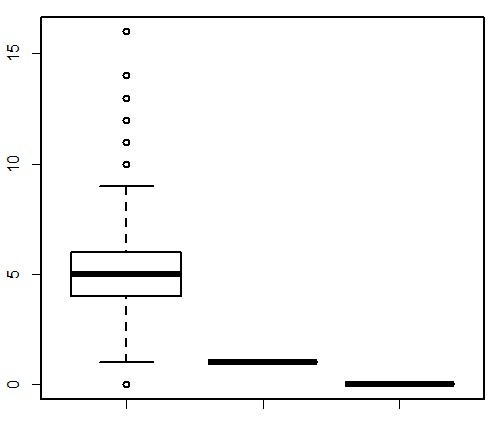
\includegraphics[height=10cm]{../fig/Tut02-57.png}
    \end{center}

\paragraph{\bf $\bullet$ Ejercicio \ref{tut02:ejercicio15},  pág. \pageref{tut02:ejercicio15}}
\label{tut02:ejercicio15:sol}\quad\\

En ambos casos, el gráfico resultante será parecido a este:
    \begin{center}
    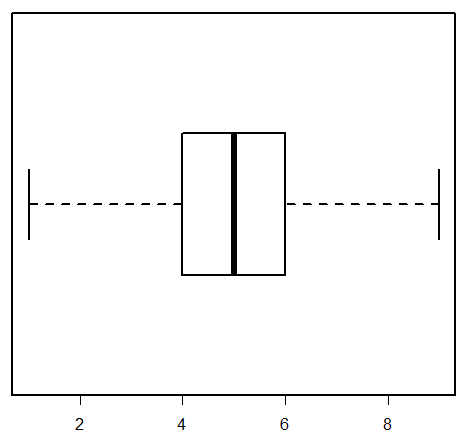
\includegraphics[height=10cm]{../fig/Tut02-58.png}
    \end{center}

\paragraph{\bf $\bullet$ Ejercicio \ref{tut02:ejercicio16},  pág. \pageref{tut02:ejercicio16}}
\label{tut02:ejercicio16:sol}\quad\\
Para la primera parte, después de comprobar que el directorio de trabajo es correcto, hacemos:
\begin{verbatim}
  > vectorEdades = read.table(file="./datos/Tut02-Edades.csv", header = FALSE)[,1]
  > (mediaEdades = mean(vectorEdades))
  [1] 6.75
\end{verbatim}
Para la segunda, las dos posibles formas de calcular la media de {\tt var3} son estas:
\begin{verbatim}
  > ( mediaVar3 = mean(var3))
  [1] 5.039231
  > ( mediaVar3 = sum(var3)/length(var3))
  [1] 5.039231
\end{verbatim}
Y, como era de esperar, el resultado es el mismo.

\paragraph{\bf $\bullet$ Ejercicio \ref{tut02:ejercicio17},  pág. \pageref{tut02:ejercicio17}}
\label{tut02:ejercicio17:sol}\quad\\
Calculamos los dos valores:
\begin{verbatim}
  > ( varMuestral = var(var3))
  [1] 4.715165
  > ( desvTipMuestral = sd(var3))
  [1] 2.171443
\end{verbatim}
Y para la comprobación que pide el ejercicio hacemos:
\begin{verbatim}
  > sqrt(varMuestral)
  [1] 2.171443
\end{verbatim}

\paragraph{\bf $\bullet$ Ejercicio \ref{tut02:ejercicio18},  pág. \pageref{tut02:ejercicio18}}
\label{tut02:ejercicio18:sol}\quad\\
Siempre podemos averiguar de que tipo de objeto se trata con la función {\tt class} de R:
\begin{verbatim}
    > class(summary(var3))
    [1] "summaryDefault" "table"
\end{verbatim}
En este caso, R nos contesta que es un tipo especial de tabla, asociado precisamente a la función {\tt summary}.


\paragraph{\bf $\bullet$ Ejercicio \ref{tut02:ejercicio22},  pág. \pageref{tut02:ejercicio22}}
\label{tut02:ejercicio22:sol}\quad\\

La tabla de frecuencia se obtiene con:
\begin{verbatim}
    > table(dado)
    dado
      1   2   3   4   5   6
    167 171 167 163 188 144
\end{verbatim}
Al ser números aleatorios, tus resultados serán distintos.

Para comprobar que {\tt dado} es un vector, ejecutamos:
\begin{verbatim}
    > class(dado)
    [1] "integer"
\end{verbatim}
y R nos informa de que, en efecto, es un vector de números enteros ({\em integer numbers}, en  inglés).

\paragraph{\bf $\bullet$ Ejercicio \ref{tut02:ejercicio23},  pág. \pageref{tut02:ejercicio23}}
\label{tut02:ejercicio23:sol}\quad\\
El generador de claves modificado es:
\begin{verbatim}
    > ( Clave = sample(c(LETTERS, letters, 0:9), size=15, replace=TRUE) )
     [1] "S" "F" "3" "U" "z" "i" "g" "L" "4" "3" "M" "S" "s" "u" "y"
\end{verbatim}
Y como aperitivo de lo que ofrece la función {\tt paste}:
\begin{verbatim}
    > paste(Clave, collapse="")
    [1] "SF3UzigL43MSsuy"
\end{verbatim}

\paragraph{\bf $\bullet$ Ejercicio \ref{tut02:ejercicio24},  pág. \pageref{tut02:ejercicio24}}
\label{tut02:ejercicio24:sol}\quad\\
El comando:
\begin{verbatim}
    > tail(dado, 1)
    [1] 1
\end{verbatim}
muestra que el último elemento es un $1$. Para ver los $10$ últimos elementos:
\begin{verbatim}
    > tail(dado, 10)
     [1] 4 6 3 4 3 5 4 2 3 1
\end{verbatim}

\paragraph{\bf $\bullet$ Ejercicio \ref{tut02:ejercicio25},  pág. \pageref{tut02:ejercicio25}}
\label{tut02:ejercicio25:sol}\quad\\
Apartado 1:
\begin{verbatim}
    > dado[16]
    [1] 3
\end{verbatim}
Apartado 2. El operador adecuado es {\tt >=}, y usamos {\tt head} para ver el comienzo de la solución:
\begin{verbatim}
    > masoIgualQue2 = dado[dado>=2]
    > head(masoIgualQue2)
    [1] 2 2 4 2 4 6
\end{verbatim}
Apartado 3:
\begin{verbatim}
    > pares = dado[dado%%2==0]
    > head(pares)
    [1] 2 2 4 2 4 6
\end{verbatim}

\paragraph{\bf $\bullet$ Ejercicio \ref{tut02:ejercicio26},  pág. \pageref{tut02:ejercicio26}}
\label{tut02:ejercicio26:sol}\quad\\

\begin{verbatim}
> (7 < 5) | (2 < 4)
[1] TRUE
\end{verbatim}


\paragraph{\bf $\bullet$ Ejercicio \ref{tut02:ejercicio27},  pág. \pageref{tut02:ejercicio27}}
\label{tut02:ejercicio27:sol}\quad\\

Recuerda que los valores booleanos se traducen en unos y ceros, y escribe:
\begin{verbatim}
    > sum(dado2 == 4)
    [1] 280
\end{verbatim}

\vspace{2cm} \hrule
\quad\\
Fin del Tutorial-02. ¡Gracias por la atención!


\end{document}
